%% LaTeX2e class for student theses
%% thesis.tex
%% 
%% Karlsruhe Institute of Technology
%% Institute for Program Structures and Data Organization
%% Chair for Software Design and Quality (SDQ)
%%
%% Dr.-Ing. Erik Burger
%% burger@kit.edu
%%
%% Version 1.3.2, 2017-08-01

%% Available page modes: oneside, twoside
%% Available languages: english, ngerman
%% Available modes: draft, final (see README)
\documentclass[twoside, english]{sdqthesis}
\graphicspath{Figures/}
\usepackage{float}
\usepackage{amsmath}
\usepackage{subfigure}
\usepackage[colorinlistoftodos,prependcaption]{todonotes}
\DeclareMathOperator*{\argmax}{arg\,max}
\DeclareMathOperator*{\argmin}{arg\,min}
\usepackage{verbatim}  % Needed for the "comment" environment to make LaTeX comments
\usepackage{vector}  % Allows "\bvec{}" and "\buvec{}" for "blackboard" style bold vectors in maths
\usepackage{colortbl}
%\usepackage[urlcolor=blue, colorlinks=true, linkcolor=black, citecolor=blue]{hyperref}  % Colours hyperlinks in blue, but this can be distracting if there are many links.
\usepackage{pgfplots}
\usepackage[]{algorithm2e}


%% ---------------------------------
%% | Information about the thesis  |
%% ---------------------------------

%% Name of the author
\author{Manuel Lang}

%% Title (and possibly subtitle) of the thesis
\title{	Data-Driven Learning of Clustering Algorithms for Image and Text Data}

%% Type of the thesis 
\thesistype{Master's Thesis}

%% Change the institute here, ``IPD'' is default
\myinstitute{Humanoids and Intelligence Systems Lab}

%% You can put a logo in the ``logos'' directory and include it here
%% instead of the SDQ logo
\grouplogo{cmu_logo}
%% Alternatively, you can disable the group logo
% TODO: Put the CMU logo in the logos directory, remove nogrouplogo
%\nogrouplogo

%% The reviewers are the professors that grade your thesis
\reviewerone{Prof. Dr. Rüdiger Dillmann}
\reviewertwo{}

%% The advisors are PhDs or Postdocs
\advisorone{}
%% The second advisor can be omitted
%\advisortwo{Dr. Sebastian Stüker}

%% Please enter the start end end time of your thesis
\editingtime{1. January 2019}{\today}

\settitle

%% --------------------------------
%% | Settings for word separation |
%% --------------------------------

%% Describe separation hints here.
%% For more details, see 
%% http://en.wikibooks.org/wiki/LaTeX/Text_Formatting#Hyphenation
\hyphenation{
% me-ta-mo-del
}

%% --------------------------------
%% | Bibliography                 |
%% --------------------------------

%% Use biber instead of BibTeX, see README
\usepackage[citestyle=numeric,style=numeric,backend=biber,sorting=none]{biblatex}
\addbibresource{Bibliography.bib}

%% ====================================
%% ====================================
%% ||                                ||
%% || Beginning of the main document ||
%% ||                                ||
%% ====================================
%% ====================================
\begin{document}

%% Set PDF metadata
\setpdf

%% Set the title
\maketitle

%% The Preamble begins here
\frontmatter

%% LaTeX2e class for student theses: Declaration of independent work
%% sections/declaration.tex
%% 
%% Karlsruhe Institute of Technology
%% Institute for Program Structures and Data Organization
%% Chair for Software Design and Quality (SDQ)
%%
%% Dr.-Ing. Erik Burger
%% burger@kit.edu
%%
%% Version 1.3.2, 2017-08-01

\thispagestyle{empty}
\null\vfill
\noindent\hbox to \textwidth{\hrulefill} 
\iflanguage{english}{I declare that I have developed and written the enclosed
thesis completely by myself, and have not used sources or means without
declaration in the text.}%
{Ich versichere wahrheitsgemäß, die Arbeit
selbstständig angefertigt, alle benutzten Hilfsmittel vollständig und genau
angegeben und alles kenntlich gemacht zu haben, was aus Arbeiten anderer
unverändert oder mit Änderungen entnommen wurde.}
 
 
%% ---------------------------------------------
%% | Replace PLACE and DATE with actual values |
%% ---------------------------------------------
\textbf{Karlsruhe, \today}
\vspace{1.5cm}
 
\dotfill\hspace*{8.0cm}\\
\hspace*{2cm}(\theauthor) 
\cleardoublepage

\setcounter{page}{1}
\pagenumbering{roman}

%% ----------------
%% |   Abstract   |
%% ----------------
 
%% For theses written in English, an abstract both in English
%% and German is mandatory.
%%
%% For theses written in German, a German abstract is sufficient.
%%
%% The text is included from the following files:
%% - sections/abstract

\includeabstract

%% ------------------------
%% |   Table of Contents  |
%% ------------------------
\tableofcontents

\listoffigures
\listoftables

%% -----------------
%% |   Main part   |
%% -----------------

\mainmatter

\chapter{Introduction}


Unsupervised grouping is used in various applications to categorize data observations into similar regions. As an example, similar documents can be combined into clusters so that for a new document or a search query, a list of corresponding documents can be suggested \cite{zamir1998web}. The same procedure can also be applied for different tasks, such as grouping products \cite{balakrishnan2018product}, searching images \cite{lin2018dimensionality} or detecting anomalies \cite{he2003discovering}. In comparison to supervised learning, the data does not must be (completely) annotated, i.e.\ potentially expensive labeling work can be omitted by using clustering algorithms. This benefit is one of the reasons why leading researchers think that unsupervised learning will be very important in the future. AI researcher and professor at NYU, Yann LeCun, wrote the following on his personal Facebook profile emphasizing the importance of unsupervised learning methods:

\blockquote{``Most of human and animal learning is unsupervised learning. If intelligence was a cake, unsupervised learning would be the cake, supervised learning would be the icing on the cake, and reinforcement learning would be the cherry on the cake. We know how to make the icing and the cherry, but we don’t know how to make the cake. We need to solve the unsupervised learning problem before we can even think of getting to true AI \cite{lecun}.''}

As the amount of available data has been increasing in the past \cite{wamba2015big}, data analysis is more often required. State-of-the-art algorithms mostly provide general complexity and runtime guarantees. Thus, worst-case guarantees have to be assumed for the given dataset. However, as large datasets do often not adapt much over time, it is very likely that also runtime and complexity of certain algorithms applied to the given data will not change much. On the other hand, it is not trivial which algorithm can then be used to obtain the optimal results, i.e.\ the optimal clusters of the given data \cite{DBLP:journals/corr/GuptaR15b}.\\

In addition, data is often split into different natural representations. For instance, images can be seen as a matrix of pixels, but also with a textual description. For machine learning experiments, it can be difficult to create a model based on various representations as it does not seem intuitive how to stack different data sources such as pixels and textual descriptions \cite{cebral2018combining}.\\

This thesis proposes several algorithms to efficiently use a linear combination of clustering algorithms to overcome the hurdle of selecting the proper algorithm for the given data. In addition, the framework this algorithm is built in\footnote{The implementation is published open-source, see \url{https://github.com/manu183/Learning-to-Link}.} will also be applied to learning a weighted linear combination of feature representations. The proposed clustering algorithms belong to a specific family that will be introduced in chapter \ref{chapter:relatedwork}. % Introduction

\chapter{Background Theory}
\label{chapter:background}

\section{Data-driven Algorithm Design}

This increasing amount of data allows us to improve the learning capabilities of machines. We know how well existing algorithms perform in general and which runtime guarantees they have. However, the algorithms' guarantees are general observations and can vary a lot between different data. Also, it is often not trivial to choose the right algorithm for the given data without extensive data engineering. In many real-world applications the data does not vary that much, e.g.\ the data for clustering websites into different types may vary quite much on a yearly base, but as this task can get executed thousands of times each second for certain search algorithms, the data will not change much. By assuming a static context, it is then possible to leverage the context to improve the algorithmic results, e.g.\ say you want to cluster person data for different genders. By having this a-priori information, you can use a k-means clustering algorithm with $k = 3$ in order to differentiate between female, male and non-binary people.\\

However, such observations are mostly not that trivial and often require more effort in order to obtain useful a-priori information. In order to cluster financial standing, one could imagine seeing different clusters depending on the age or the education. But how many clusters would result here? The data has to be processed and evaluated for different values in this case.\\

Once our algorithm performs well for our data and our tasks, we then want to transfer the gained knowledge to different tasks. Say the algorithm already learned how to differentiate images of the handwritten digits zero, one and two, the same algorithm should then be able to apply the gained knowledge to distinguish between other handwritten digits too. The gained knowledge is some kind of learned data, that can for example be the feature representation of a Convolutional Neural Network, where a potential goal can be to transfer the representation knowledge to another classification task.\\

For clustering tasks learned knowledge could be a number of clusters, a good feature representation for the input data or other useful information that allows performing similar clustering tasks better by transferring the knowledge.

\section{Linkage-based hierarchical clustering.}

This thesis focuses on agglomerative hierarchical clustering, i.e.\ clustering algorithms that merge clusters starting from each cluster as its own point until all points belong to the same cluster. In each iteration, the two clusters with the closest distance get merged together. As there are various clustering algorithms, there also are various distance measurements. One way to describe the distance between two clusters, say $X$ and $Y$, is by defining a linkage between them. There are three main methods to do so \cite{Manning:2008:IIR:1394399}.

\paragraph{Single Linkage.}

Single linkage defines a distance between two clusters $X$ and $Y$ as the distance between the two nearest points of these clusters (see equation \ref{eq:singlelinkage}).

\begin{equation}
    \begin{aligned}
        d_{SL}(X,Y) = \min\limits_{x \in X, y \in Y} d(x,y)
    \end{aligned}
    \label{eq:singlelinkage}
\end{equation}

\paragraph{Complete Linkage.}

Complete linkage defines a distance between two clusters $X$ and $Y$ as the distance between the two farthest points of these clusters (see equation \ref{eq:completelinkage}).

\begin{equation}
    \begin{aligned}
        d_{CL}(X,Y) = \max\limits_{x \in X, y \in Y} d(x,y)
    \end{aligned}
    \label{eq:completelinkage}
\end{equation}

\paragraph{Average Linkage.}

Average linkage defines a distance between two clusters $X$ and $Y$ as the average distance between all points $x \in X$ and all points $y \in Y$ (see equation \ref{eq:averagelinkage}).

\begin{equation}
    \begin{aligned}
        d_{AL}(X,Y) = \frac{1}{|X||Y|}\sum\limits_{x \in X, y \in Y} d(x,y)
    \end{aligned}
    \label{eq:averagelinkage}
\end{equation}

Figure \ref{fig:linkage_types} demonstrates which points are used for the different linkage strategies using two exemplary clusters.

\begin{figure}[h]
    \centering
    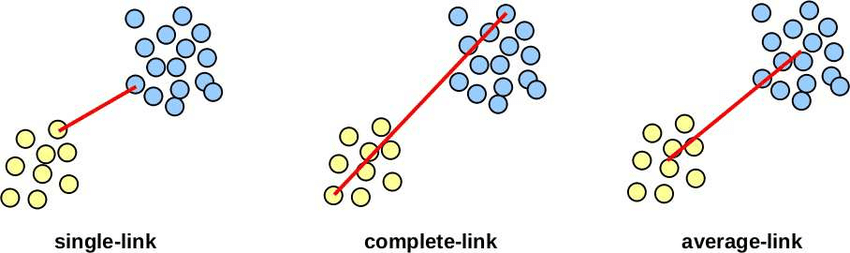
\includegraphics[width=0.8\textwidth]{images/linkage_types}
    \caption{To calculate the distance between two clusters, single linkage calculates the nearest neighbor distance, complete linkage uses the farthest neighbor and average linkage calculates the average distance over all points \cite{linkage_types}.}
    \label{fig:linkage_types}
\end{figure}

\paragraph{Effects of different linkage strategies.}

Depending on the linkage strategy, the pairwise distances between all $N$ clusters $C_1, ..., C_N$ will be different. As the clustering algorithm merges the closest pair of clusters in each iteration, the merging clusters $C_i$ and $C_j$ with $i, j \in 1,...,N$ might vary as shown in figure \ref{fig:linkage_effects}, where ten clusters $C_0, ..., C_9$ get clustered with bottom-up hierarchical clustering using the Euclidean distance as the pointwise distance $d(x,y)$ to calculate the pairwise distance according to the three mentioned linkage strategies.

\begin{figure}[h]
    \centering
    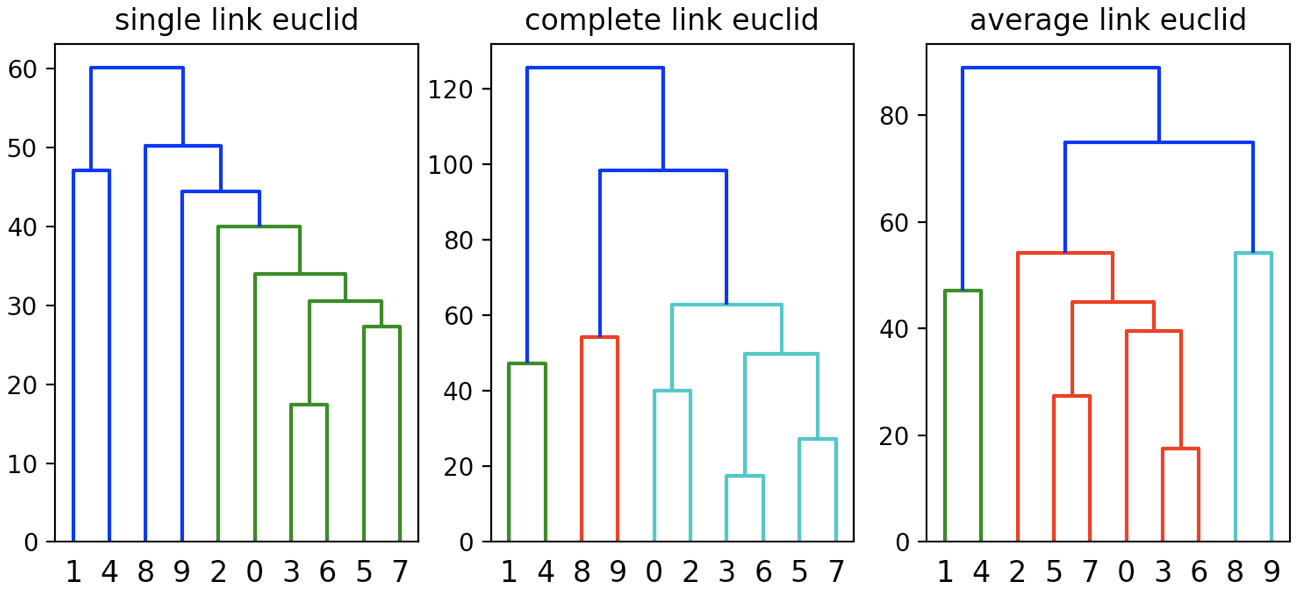
\includegraphics[width=0.8\textwidth]{images/linkage_effects}
    \caption{Different distance measurements often result in different merges for bottom-up hierarchical clustering algorithms. The three discussed linkage strategies result in three different clusterings.}
    \label{fig:linkage_effects}
\end{figure}

As different points are merged together, this also means that the clustering may have a different quality. This thesis compares the clusterings' quality for different data by introducing algorithms to efficiently determine the quality not only for these linkage strategies but also for their linear combinations.

\section{Generating Feature Representations}

In order to improve the overall clustering performance, this work uses several techniques to obtain better feature representations of text and image data. 

\subsection{Text Features}

To cluster different words, there are several ways to create a difference measurement of these words. 

\paragraph{Word Edit Distance.} A rather simple approach would be to calculate the edit distance that describes the difference of the characters in the words \cite{ristad1998learning}. However, this approach does not contain any semantic information, i.e.\ synonyms will have a larger distance than wanted. For example the edit distance between loan and moan is very small ($wed(loan, moan) = 1$) where the edit distance between loan and credit is larger ($wed(loan, credit) = 6)$.\\ 

\paragraph{Word Embeddings.} This motivates to leverage contextual information, where we can use several pre-trained models on different datasets. Stanford's GloVe provides such models that incorporate knowledge from Wikipedia and social networks \cite{pennington2014glove}. Figure \ref{fig:glove} shows examples for why these embeddings give a helpful feature representation.\\

\begin{figure}[h]
\centering
\begin{minipage}{.3\textwidth}
  \centering
  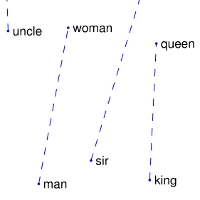
\includegraphics[width=\linewidth]{images/glove_mw}
\end{minipage}
\begin{minipage}{.3\textwidth}
  \centering
  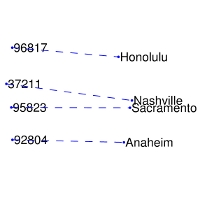
\includegraphics[width=\linewidth]{images/glove_cz}
\end{minipage}
\begin{minipage}{.3\textwidth}
  \centering
  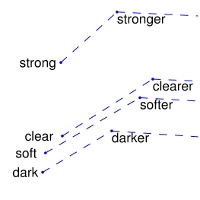
\includegraphics[width=\linewidth]{images/glove_cs}
\end{minipage}
\caption{Word embeddings give insightful correlations between similar and different words. For example, we can obtain several relations between female and male people, between zip codes and cities or between comparative and superlative words \cite{pennington2014glove}.}
\label{fig:glove}
\end{figure}

\paragraph{Bag of Contexts.} In addition, CMU's Machine Learning Department provides another way to compare words. Their Never-Ending Language Learner provides information in which contexts certain words are used online \cite{nell_pairs}, e.g.\ by considering that both Pittsburgh and Karlsruhe are used in the one same context ``is a city'' and Pittsburgh and Philadelphia share additional contexts such as ``belongs to the state Pennsylvania'', we can conclude that Pittsburgh has a higher correlation to Philadelphia than to Karlsruhe. We can then create a corpus containing all different contexts. Similar to the bag-of-words approach, we can then count the occurrences of the words in the corpus' contexts. However, the resulting data is very sparse and Euclidean distance will not work well to compare the ``bag-of-contexts'' representations, i.e.\ other measurements such as the cosine distance are preferred.

\subsection{Image Features}
\label{sec:imagefeatures}

Similarly, there also exist ways to extract useful features from image data. In particular, this work focuses on neutral networks that learn to represent images in a way that images of different classes can be seperated well where images of the same class might share similar features.\\

\paragraph{CNN Features.} As a primary example, we use Convolutional Neural Network (CNN) architectures that learn to represent images with convolutional, pooling and activation layers and later map the representations to target classes with fully-connected layers. In this way, we can cut off the fully-connected layers to extract lower-dimensional feature representations for the input image data. Figure \ref{fig:cnnfeatures} visualizes such features learned on the ImageNet dataset \cite{krizhevsky2012imagenet}.

\begin{figure}[h]
    \centering
    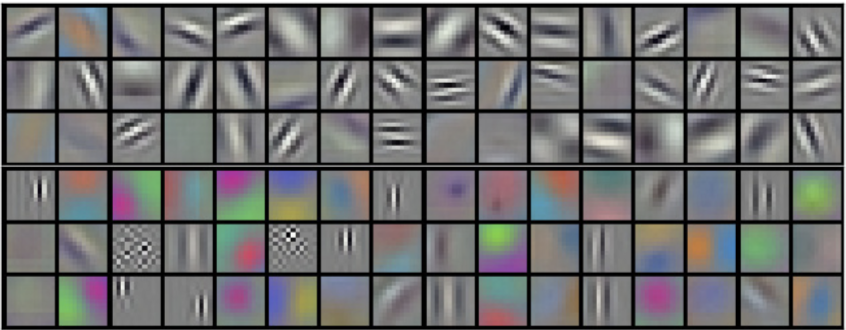
\includegraphics[width=0.8\textwidth]{images/cnn_features}
    \caption{Convolutional Neural Networks learn to represent images in lower-dimensional feature maps by applying convolutions to the image and averaging local neighborhoods (pooling) \cite{krizhevsky2012imagenet}.}
    \label{fig:cnnfeatures}
\end{figure} % Background Theory 

\chapter{Related Work}
\label{chapter:relatedwork}

\section{Data-driven Algorithm Design}

We know how well existing algorithms perform in general and which complexity guarantees they have. However, the algorithms' guarantees are general observations and can vary a lot between different data. Also, it is often not trivial to choose the right algorithm for the given data without extensive data engineering. In many real-world applications, the data does not vary that much. For instance, the data for clustering websites into different types may vary quite much on a yearly base, but as this task can get executed thousands of times each second for certain search algorithms, the data will not change much. By assuming a static context, it is then possible to leverage the context to improve the algorithmic results. Empirical work without much theoretical foundation exists in domains such as artificial intelligence \cite{Xu:2008:SPA:1622673.1622687}, computational biology \cite{deblasio2018adaptive} or game theory \cite{likhodedov2004methods}. However, in this work we focus on clustering tasks, e.g.\ say we want to cluster person data for different genders. By having apriori information, we can use a k-means clustering algorithm with $k = 3$ in order to differentiate between female, male and non-binary people.\\

However, such observations are mostly not trivial and often require more effort in order to obtain useful apriori information. In order to cluster financial standing, one could imagine seeing different clusters depending on the age or the education. But how many clusters would result here? The data has to be processed and evaluated for different values in this case.\\

Once our algorithm performs well for our data and our tasks, we then want to transfer the gained knowledge to different tasks. Say the algorithm has already learned how to differentiate images of the handwritten digits zero, one and two, the same algorithm should then be able to apply the gained knowledge to distinguish between other handwritten digits too. The gained knowledge is some kind of learned data, that for example can be the feature representation of a Convolutional Neural Network, where a potential goal can be to transfer the representation knowledge to another classification task. For clustering tasks learned knowledge could be a number of clusters, a good feature representation for the input data or other useful information that allows performing similar clustering tasks better by transferring the knowledge.\\

Data-driven learning is in general closely related to hyperparameter tuning \cite{hutter2015beyond}, where we try to find the best value of a given parameter to optimize the overall quality, automated machine learning \cite{lacoste2014sequential,liu2018very}, where we perform end-to-end learning for given data, and meta learning \cite{alexandros2001model}, where we try to extract meta-knowledge as one step of the learning process.

\section{Linkage-based Hierarchical Clustering}

This thesis focuses on agglomerative hierarchical clustering, i.e.\ clustering algorithms that merge clusters starting from each point as its own cluster until all points belong to the same cluster. In each iteration, the two clusters with the closest distance get merged together. As there are various clustering algorithms, there are also various distance measurements which are widely used in practice and optimal in many cases \cite{awasthi2017local,saeed2003software,white2010alignment,awasthi2012center,balcan2016clustering,grosswendt2017improved}. One popular way to describe the distance between two clusters is by defining a linkage between them. There are three main methods to do so \cite{Manning:2008:IIR:1394399}.

\paragraph{Single Linkage.}

Single linkage defines a distance between two clusters $X$ and $Y$ as the distance between the two nearest points of these clusters.

\begin{equation*}
    \begin{aligned}
        d_{SL}(X,Y) = \min\limits_{x \in X, y \in Y} d(x,y)
    \end{aligned}
    \label{eq:singlelinkage}
\end{equation*}

\paragraph{Complete Linkage.}

Complete linkage defines a distance between two clusters $X$ and $Y$ as the distance between the two farthest points of these clusters.

\begin{equation*}
    \begin{aligned}
        d_{CL}(X,Y) = \max\limits_{x \in X, y \in Y} d(x,y)
    \end{aligned}
    \label{eq:completelinkage}
\end{equation*}

\paragraph{Average Linkage.}

Average linkage defines a distance between two clusters $X$ and $Y$ as the average distance between all points $x \in X$ and all points $y \in Y$.

\begin{equation*}
    \begin{aligned}
        d_{AL}(X,Y) = \frac{1}{|X||Y|}\sum\limits_{x \in X, y \in Y} d(x,y)
    \end{aligned}
    \label{eq:averagelinkage}
\end{equation*}

Figure \ref{fig:linkage_types} shows how the distances between the two exemplary clusters get calculated with the different linkage strategies.

\begin{figure}[h]
    \centering
    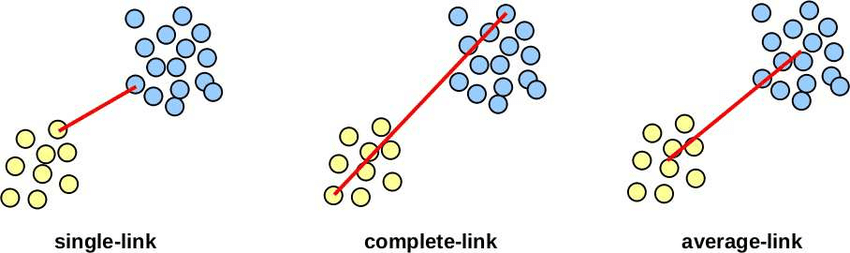
\includegraphics[width=0.8\textwidth]{images/linkage_types}
    \caption{To calculate the distance between two clusters, single linkage calculates the nearest neighbor distance, complete linkage uses the farthest neighbor and average linkage calculates the average distance over all points \cite{linkage_types}.}
    \label{fig:linkage_types}
\end{figure}

\paragraph{Effects of different linkage strategies.}

Depending on the linkage strategy, the pairwise distances between all $N$ clusters $C_1, ..., C_N$ are different for all clusters containing more than one point. As the clustering algorithm merges the closest pair of clusters in each iteration, the merging clusters $C_i$ and $C_j$ with $i, j \in 1,...,N$ might vary as shown in figure \ref{fig:linkage_effects}. There, ten clusters $C_0, ..., C_9$ get clustered with bottom-up hierarchical clustering using the Euclidean distance as the pointwise distance $d(x,y)$ to calculate the pairwise distance according to the three mentioned linkage strategies.

\begin{figure}[h]
    \centering
    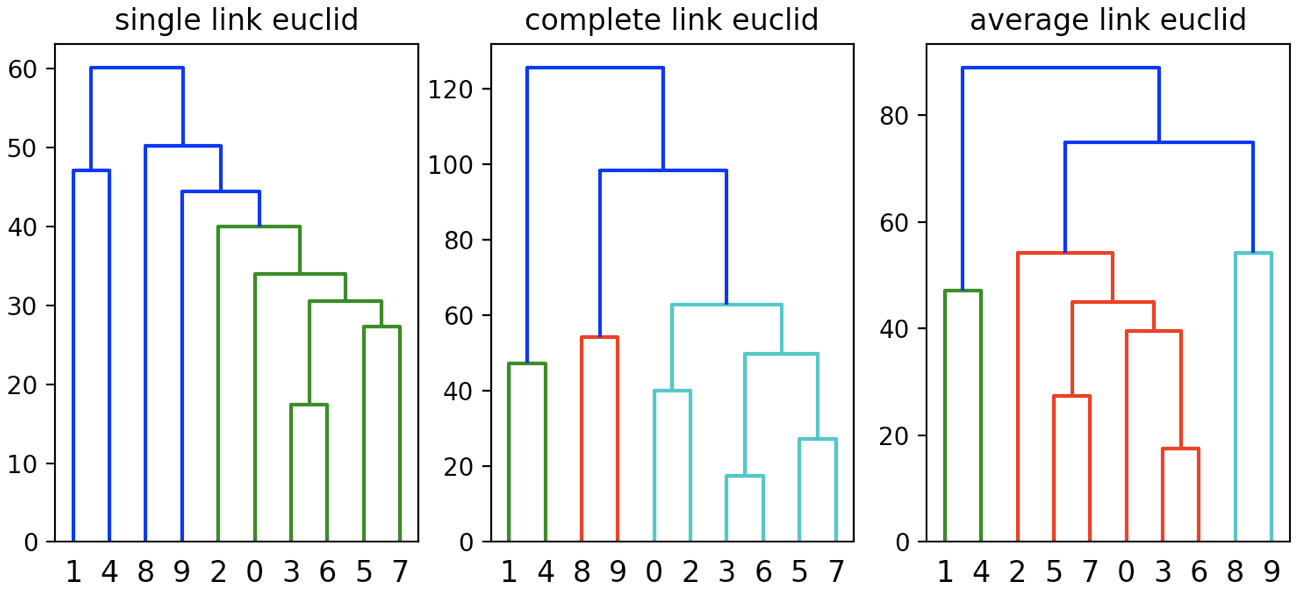
\includegraphics[width=0.8\textwidth]{images/linkage_effects}
    \caption{Different distance measurements often result in different merges for bottom-up hierarchical clustering algorithms. The three discussed linkage strategies result in three different clusterings.}
    \label{fig:linkage_effects}
\end{figure}

As different points are merged together, this also means that the clustering may have a different quality. This thesis compares the clusterings' quality for different data by introducing algorithms to efficiently determine the quality not only for these linkage strategies but also for their linear combinations.

\section{Generating Feature Representations}

In order to improve the overall clustering performance, this work uses several techniques to obtain better feature representations of text and image data. 

\subsection{Text Features}

To cluster different words, there are several ways to create a difference measurement of these words. 

\paragraph{Word Edit Distance.} A rather simple approach is to calculate the edit distance that describes the difference between the characters in the words \cite{ristad1998learning}. However, this approach does not contain any semantic information, i.e.\ synonyms will have a larger distance than wanted. For example the edit distance between loan and moan (two words with a very different meaning) is very small ($wed(loan, moan) = 1$) where the edit distance between loan and credit (two words with a very similar meaning) is larger ($wed(loan, credit) = 6)$. 

\paragraph{Word Embeddings.} This motivates to leverage contextual information, where we can use several pre-trained models on different datasets. GloVe provides such models that incorporate knowledge from Wikipedia and social networks \cite{pennington2014glove}. Figure \ref{fig:glove} shows examples of why these embeddings give a helpful feature representation. 

\begin{figure}[h]
\centering
\begin{minipage}{.3\textwidth}
  \centering
  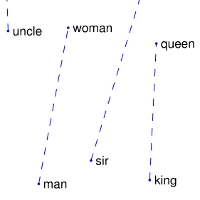
\includegraphics[width=\linewidth]{images/glove_mw}
\end{minipage}
\begin{minipage}{.3\textwidth}
  \centering
  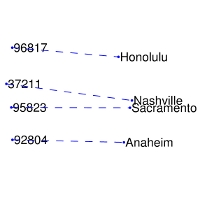
\includegraphics[width=\linewidth]{images/glove_cz}
\end{minipage}
\begin{minipage}{.3\textwidth}
  \centering
  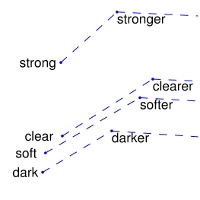
\includegraphics[width=\linewidth]{images/glove_cs}
\end{minipage}
\caption{Word embeddings give insightful correlations between similar and different words. For example, we can obtain several relations between female and male people, between zip codes and cities or between comparative and superlative words \cite{pennington2014glove}.}
\label{fig:glove}
\end{figure}

\paragraph{Bag-of-Contexts.} In addition, CMU's Machine Learning Department provides another way to compare words. Their Never-Ending Language Learner provides information in which contexts certain words are used \cite{nell_pairs}, e.g.\ by considering that both Pittsburgh and Karlsruhe are used in the same context ``\_ is a city'', and Pittsburgh and Philadelphia share additional contexts such as ``\_ belongs to the state Pennsylvania'', we can conclude that Pittsburgh has a higher correlation to Philadelphia than to Karlsruhe. We can then create a corpus containing all different contexts. Similar to the bag-of-words approach \cite{bow}, we then count the occurrences of the words in the corpus' contexts. However, the resulting data is very sparse and the Euclidean distance might not work well to compare the ``bag-of-contexts'' representations, i.e.\ other measurements such as the cosine distance are preferred.

\subsection{Image Features}
\label{sec:imagefeatures}

Similarly, there also exist ways to extract useful features from image data. In particular, this work focuses on neural networks that learn to represent images in a way that images of different classes can be separated well where images of the same class might share similar features. 

\paragraph{Neural Network Features.} As a primary example, we use Convolutional Neural Network (CNN) architectures that learn to represent images with convolutional, pooling and activation layers and later map the representations to target classes with fully-connected layers. In this way, we can cut off the fully-connected layers to extract lower-dimensional feature representations for the input image data. Figure \ref{fig:cnnfeatures} visualizes such features learned on the ImageNet dataset \cite{krizhevsky2012imagenet}.

\begin{figure}[h]
    \centering
    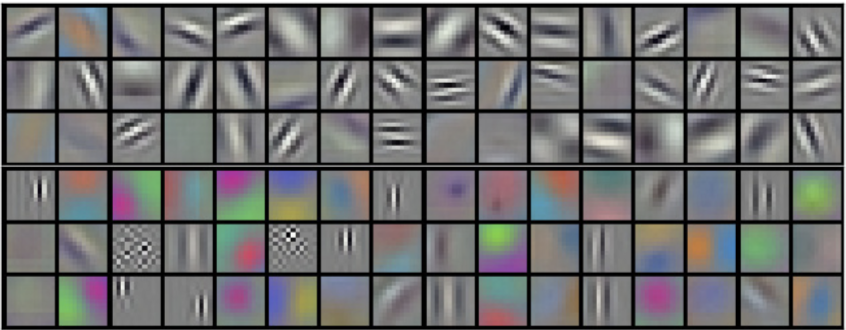
\includegraphics[width=0.7\textwidth]{images/cnn_features}
    \caption{Convolutional Neural Networks learn to represent images in lower-dimensional feature maps by applying convolutions to the image and averaging local neighborhoods (pooling) \cite{krizhevsky2012imagenet}.}
    \label{fig:cnnfeatures}
\end{figure}

\section{Data-Driven Clustering}

As briefly discussed earlier, it is not trivial to find the best algorithm for a given clustering task. While there already is empirical work in data-driven algorithm selection in certain domains such as choosing the step size in gradient descent \cite{DBLP:journals/corr/GuptaR15b}, this thesis focuses on the earlier discussed bottom-up hierarchical clustering with the three different linkage strategies. In practice, there exists a variety of additional clustering algorithms that are parameterized, however data-driven methods only exist to some extent, e.g.\ for calculating the seed points of k-means efficiently \cite{arthur2007k}.\\

As this work tries to select from a family of strategies, we first look at formulations that describe the given families. Balcan et al. introduced two infinite families to interpolate between different linkage strategies, such as shown in equations \ref{eq:algfam1} and \ref{eq:algfam2} \cite{DBLP:journals/corr/BalcanNVW16}.

\begin{equation}
    \begin{aligned}
        \mathcal{A}_1 = \left\{ \left( \min\limits_{u \in A, v \in B} (d(u,v))^\alpha + \max\limits_{u \in A, v \in B} (d(u,v))^\alpha\ \right)^{1 / \alpha} \middle| \alpha \in \mathbb{R} \cup \{\infty, -\infty\} \right\}
    \end{aligned}
    \label{eq:algfam1}
\end{equation}

Equation \ref{eq:algfam1} shows a distance in the range between single linkage ($\alpha = -\infty$) and complete linkage ($\alpha = \infty$). They also show that $\mathbb{R} \cup \{\infty, -\infty\}$ contains a maximum of $O(n^8)$ different intervals, where each interval $[\alpha_{lo}, \alpha_{hi}]$ represents a different merging behavior, i.e.\ a different clustering.

\begin{equation}
    \begin{aligned}
        \mathcal{A}_2 = \left\{ \left( \frac{1}{|A| |B|} \sum\limits_{u \in A, v \in B} (d(u,v))^\alpha \right)^{1 / \alpha} \middle| \alpha \in \mathbb{R} \cup \{\infty, -\infty\} \right\}
    \end{aligned}
    \label{eq:algfam2}
\end{equation}

Equation \ref{eq:algfam2} will also result in single linkage for $\alpha = - \infty$ and complete linkage for $\alpha = \infty$. In addition, the family $\mathcal{A}_2$ also contains the definition of average linkage ($\alpha = 1$). However, the guarantee for maximum $O(n^8)$ intervals does not apply to this family. A formal guarantee will be $O(n^4 2^n)$, but this thesis will show that the empirical results are much better than the actual formal guarantee.\\

Balcan et. al also provide a solution to calculate all different merges of $\mathcal{A}_1$, however this approach solves the mathematical equations and leads to the same clusters being used for a merge quite often. As our solution only evaluates cases where different pairs of clusters get merged, the algorithm described in the following section has a lower runtime as well as a lower complexity. % Related Work

\chapter{Efficient Algorithm Selection}
\label{chapter:alphalinkage}

\todo[inline]{more formal definitions and lemmas}

We define $\alpha$ as the parameter with which the output of an algorithm is weighted. In this chapter we propose different distance measures depending on the weight parameter $\alpha$ that allows us interpolating between different linkage strategies in a way similar to the proposed by Balcan et al. \cite{DBLP:journals/corr/BalcanNVW16}, where a infinite interval was proposed.

To have a real application, we need to have a finite set of intervals. So we interpolate between one algorithm with $\alpha = 0$ and another algorithm with $\alpha = 1$, where for $\alpha = 0$ the result will be the result of algorithm 1 and for $\alpha = 1$ the result of algorithm 2.

\section{Linear Interpolation between two different linkage strategies}

Interpolating between two of the three mentioned linkage strategies results in three different algorithmic settings. In the first setting we are using the single linkage distance $d_{SL}(X,Y)$ and the complete linkage distance $d_{CL}(X,Y)$. By combining the two distances we can create a linear model that ranges from $\alpha = 0$ (single linkage) to $\alpha = 1$ (complete linkage) resulting in equation \ref{eq:singlecomplete}.

\begin{equation}
    \begin{aligned}
        d_{SC}(X,Y,\alpha) &= (1 - \alpha) \cdot d_{SL}(X,Y) + \alpha \cdot d_{CL}(X,Y)\\
        &= (1 - \alpha) \min\limits_{x \in X, y \in Y} d(x,y) + \alpha \max\limits_{x \in X, y \in Y} d(x,y)
    \end{aligned}
    \label{eq:singlecomplete}
\end{equation}

Equivalently we can interpolate between the single linkage distance $d_{SL}(X,Y)$ and the average linkage distance $d_{AL}(X,Y)$ instead of the complete linkage distance $d_{CL}(X,Y)$ for $\alpha = 1$ resulting in equation \ref{eq:singleaverage}. 

\begin{equation}
    \begin{aligned}
        d_{SA}(X,Y,\alpha) &= (1 - \alpha) \cdot d_{SL}(X,Y) + \alpha \cdot d_{AL}(X,Y)\\
        &= (1 - \alpha) \min\limits_{x \in X, y \in Y} d(x,y) + \alpha \frac{1}{|X| |Y|}\sum\limits_{x \in X, y \in Y} d(x,y)
    \end{aligned}
    \label{eq:singleaverage}
\end{equation}

The last of the three settings describes the interpolation between the average linkage distance $d_{AL}(X,Y)$ and the complete linkage distance $d_{CL}(X,Y)$ resulting in equation \ref{eq:averagecomplete}.

\begin{equation}
    \begin{aligned}
        d_{AC}(X,Y,\alpha) &= (1 - \alpha) \cdot d_{AL}(X,Y) + \alpha \cdot d_{CL}(X,Y)\\
        &= (1 - \alpha) \frac{1}{|X| |Y|}\sum\limits_{x \in X, y \in Y} d(x,y) + \alpha \max\limits_{x \in X, y \in Y} d(x,y)
    \end{aligned}
    \label{eq:averagecomplete}
\end{equation}

% \section{Linear Interpolation between three different linkage strategies}

\section{Proposed Algorithms}

\todo[inline]{use other algorithm environment}

Our goal is to find an algorithm that determines all different behavior depending on different values of $\alpha$. To do so, we propose different algorithms. The goal of the first algorithm is to divide the interval of $\alpha \in [\alpha_{lo}, \alpha_{hi}]$ to subintervals where the behavior is consistent within each interval. 

\begin{algorithm}[H]
    \KwData{input data $p_1, ..., p_N$, initial states $st$}
    \KwResult{$k$ intervals $[\alpha_0, \alpha_1], ..., [\alpha_{k-1},\alpha_k]$}
    \For{$iteration\gets1$ \KwTo $N-1$}{
        \ForEach{state $s \in st$}{%
        remove state $s$\;
        $cand_1, cand_2 \gets $find merge candidates for $s.\alpha_{lo}$ and $s.\alpha_{hi}$\;
        \eIf{$cand_1 == cand_2$}{
          $ms \gets$ merge $cand_1$\;
          add state $ms$ with interval $[\alpha_{lo},\alpha_{hi}]$ to the end of $st$\;
          }{
          $\alpha_{split} \gets$ calculate split\;
          $s_1 \gets$ merge $cand_1$\;
          $s_2 \gets$ merge $cand_2$\;
          add state $s_1$ with interval $[\alpha_{lo},\alpha_{split}]$ to the end of $st$\;
          add state $s_2$ with interval $[\alpha_{split},\alpha_{hi}]$ to the end of $st$\;
         }
        }
      }
    \caption{We calculate all from splits resulting different intervals between $\alpha_{lo}$ and $\alpha_{hi}$, merge the resulting clusters and do so until each state contains only one cluster with all points.}
    \label{alg:alphalinkage1}
\end{algorithm}

Starting from an interval $\alpha \in [\alpha_{lo}, \alpha_{hi}]$, we calculate the merging clusters by $\min\limits_{X, Y} d(X,Y,\alpha)$ for both the minimum $\alpha_{li}$ and the maximum $\alpha_{hi}$ of the interval. In case both values of $\alpha$ return the same pair of merging clusters $X$ and $Y$, we merge $X$ and $Y$. In case the values of $\alpha_{lo}$ and $\alpha_{hi}$ lead to different merges, we can calculate a value $\alpha_{split}$ where we know that for values of $\alpha \in [\alpha_{lo}, alpha_{split})$ we merge the clusters found for $\min\limits_{X, Y} d(X,Y,\alpha_{lo})$ and for values of $\alpha \in [\alpha_{split}, alpha_{hi}]$ we merge the clusters found for $\min\limits_{X, Y} d(X,Y,\alpha_{hi})$. In order to calculate the value of $\alpha_{split}$ we can equalize the distance functions of the merges of clusters $X, Y$ and the clusters $A, B$ (say $\alpha_{lo}$ leads to merging $X$ and $Y$ and $\alpha_{hi}$ leads to merging $A$ and $B$) as seen in equation \ref{eq:equalize}. 

\begin{equation}
    \begin{aligned}
        d(X,Y,\alpha_{split}) = d(A,B,\alpha_{split})
    \end{aligned}
    \label{eq:equalize}
\end{equation}

Applying \ref{eq:equalize} to a concrete example of distance functions leads to a concrete calculation for the value of $\alpha_{split}$. Equation \ref{eq:equalizesc} shows the calculation for the in equation \ref{eq:singlecomplete} introduced $d_{SC}$.

\begin{equation}
    \begin{aligned}
        \begin{gathered}
        d_{SC}(X,Y,\alpha_{split}) = d_{SC}(A,B,\alpha_{split})\\
        (1 - \alpha_{split}) \min\limits_{x \in X, y \in Y} d(x,y) + \alpha_{split} \max\limits_{x \in X, y \in Y} d(x,y) = \\
        = (1 - \alpha_{split}) \min\limits_{a \in A, b \in B} d(a,b) + \alpha_{split} \max\limits_{a \in A, b \in B} d(a,b)\\
        (- \alpha_{split}) \min\limits_{x \in X, y \in Y} d(x,y) + \alpha_{split} \max\limits_{x \in X, y \in Y} d(x,y) + \alpha_{split} \min\limits_{a \in A, b \in B} d(a,b) - \alpha_{split} \max\limits_{a \in A, b \in B} d(a,b) =\\
        = - \min\limits_{x \in X, y \in Y} d(x,y) + \min\limits_{a \in A, b \in B} d(a,b)\\
        \alpha_{split} (- \min\limits_{x \in X, y \in Y} d(x,y) + \max\limits_{x \in X, y \in Y} d(x,y) + \min\limits_{a \in A, b \in B} d(a,b) - \max\limits_{a \in A, b \in B} d(a,b)) =\\
        = - \min\limits_{x \in X, y \in Y} d(x,y) + \min\limits_{a \in A, b \in B} d(a,b)\\
        \alpha_{split} = \frac{- \min\limits_{x \in X, y \in Y} d(x,y) + \min\limits_{a \in A, b \in B} d(a,b)}{- \min\limits_{x \in X, y \in Y} d(x,y) + \max\limits_{x \in X, y \in Y} d(x,y) + \min\limits_{a \in A, b \in B} d(a,b) - \max\limits_{a \in A, b \in B} d(a,b)}
    \end{gathered}
    \end{aligned}
    \label{eq:equalizesc}
\end{equation}

After knowing the exact consistent range, we split the clusters for the different states and then calculate the merge candidates for the start and the end of the new intervals again. We can show the different possible merges in a tree of executions, where each node represents one interval $[\alpha_{lo}, \alpha_{hi}]$ where the same clusters get merged (see figure \ref{fig:toe}).

\begin{figure}[H]
    \centering
    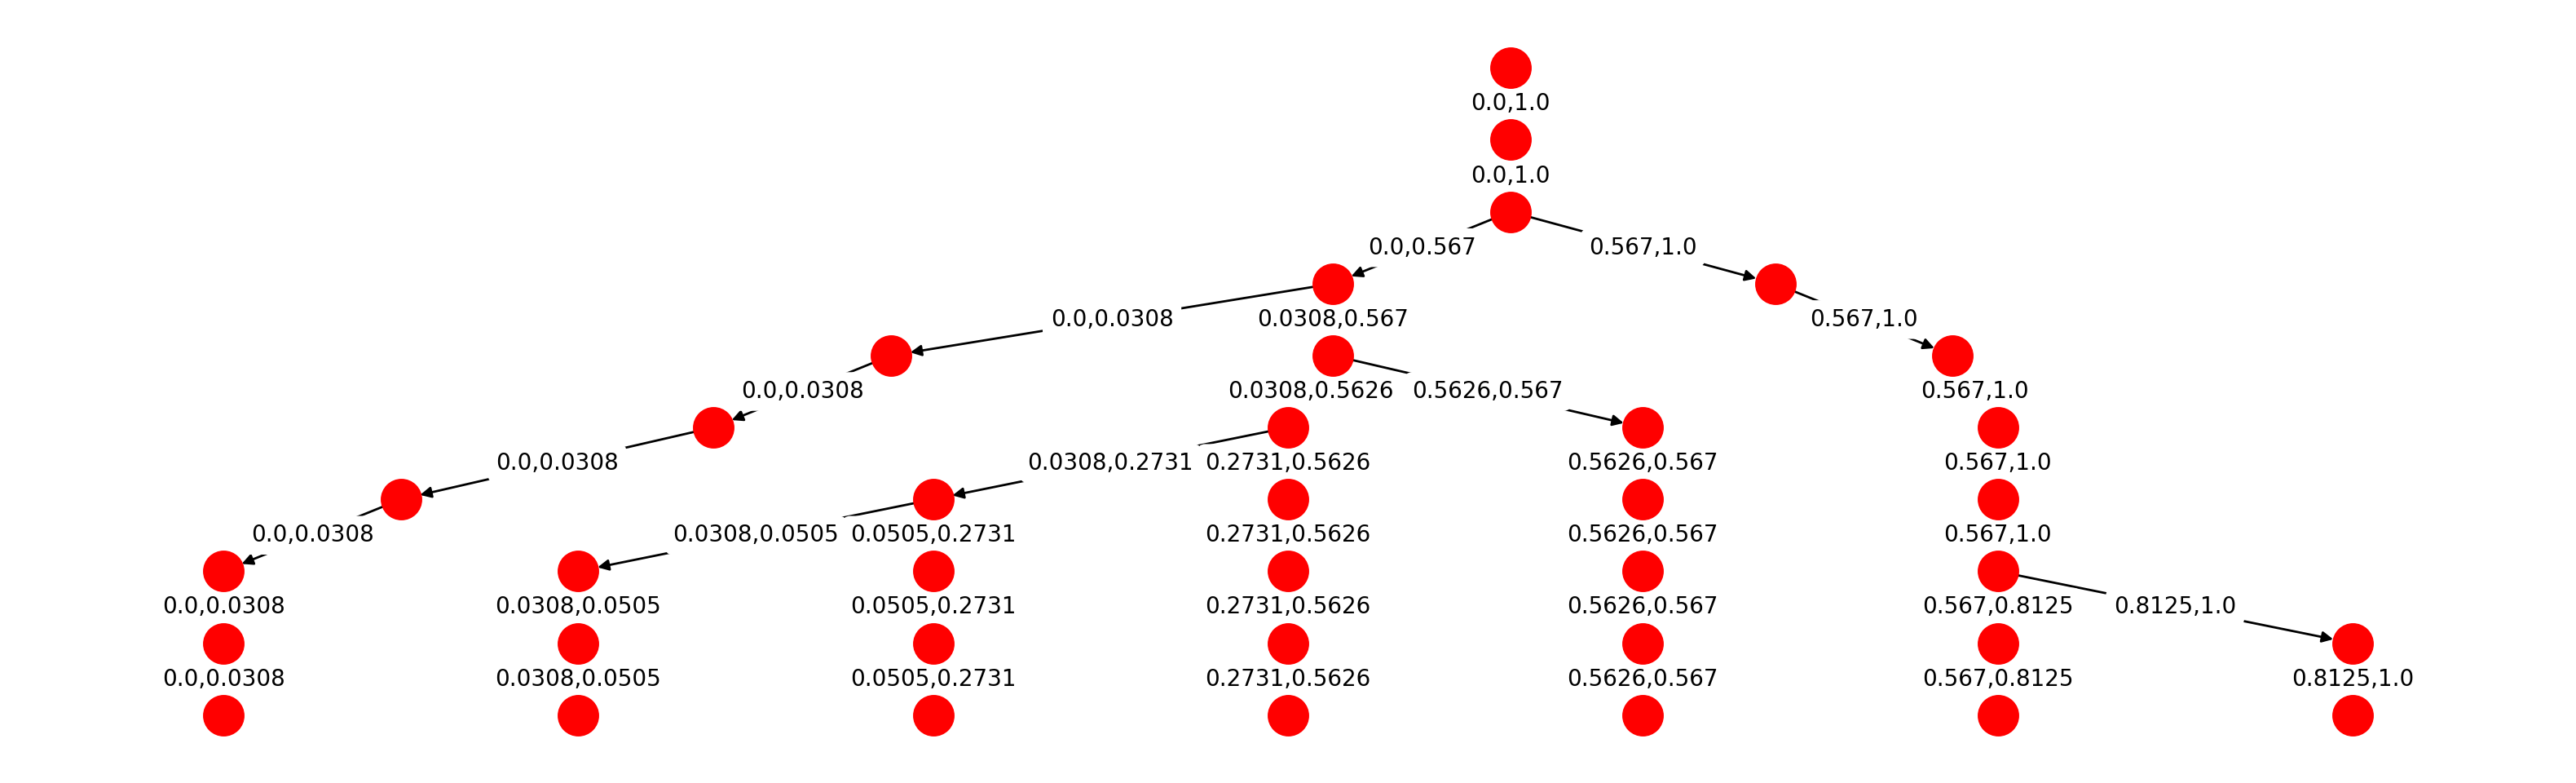
\includegraphics[width=\textwidth]{images/res_tree}
    \caption{Different values of $\alpha$ lead to different merges. We calculate a tree where we start with the entire range $[\alpha_{lo}, \alpha_{hi}]$ and split the interval into all different subintervals with consistent merges.}
    \label{fig:toe}
\end{figure}

We perform the described procedure for iterations $i = count(points) -1$ times until only one cluster containing all points is left. All the leaf nodes in the resulting tree of executions then represent one interval $[\alpha_{lo}, \alpha_{hi}]$ where the clustering is consistent within the interval and each interval contains a different clustering.\\

However just calculating the split values in a range $[\alpha_{lo}, \alpha_{hi}]$ does not necessarily yield to the best possible solution. One of these examples is demonstrated in figure \ref{fig:notoptimal}, where the blue line for the constant value of $d$ will not be considered, only the lines $\alpha \in [\alpha_{lo}, alpha_{split})$ (red) and $\alpha \in [\alpha_{split}, alpha_{high}]$ (black) will be.

\begin{figure}[H]
    \centering
    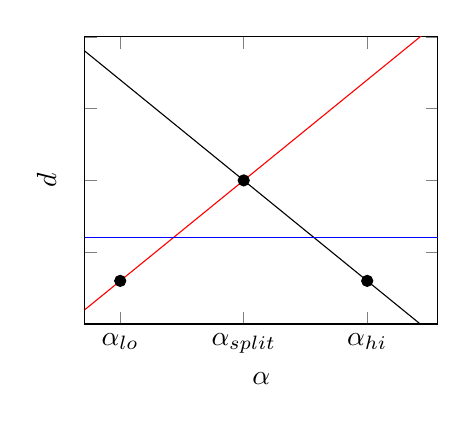
\begin{tikzpicture}
        \begin{axis}[ 
        xlabel=$\alpha$,
        ylabel={$d$},
        xmin=0.4,
        xmax=0.9,
        xtick={0.45,0.625,0.8},
        xticklabels={$\alpha_{lo}$, $\alpha_{split}$, $\alpha_{hi}$},
        width=0.5\textwidth,
        yticklabels={,,}
        ] 
        \addplot[mark=none, red] {-3+8*x}; 
        \addplot[mark=none, black] {-8*x+7};
        \addplot[mark=none, blue] {1.2};
        \addplot [only marks] table {
        0.45   0.6
        0.625  2
        0.8    0.6
        };
        \end{axis} 
    \end{tikzpicture}
    \caption{Simply calculating the split values between the start and the end value of the range $[\alpha_{lo}, \alpha_{hi}]$ will not necessarily lead to the optimal values. By doing so, the blue line (constant $d$ value) will not be considered.}
    \label{fig:notoptimal}
\end{figure}

In order to solve this, we can recursively check each resulting interval again if it contains different merging behaviors.

\begin{figure}[H]
    \centering
    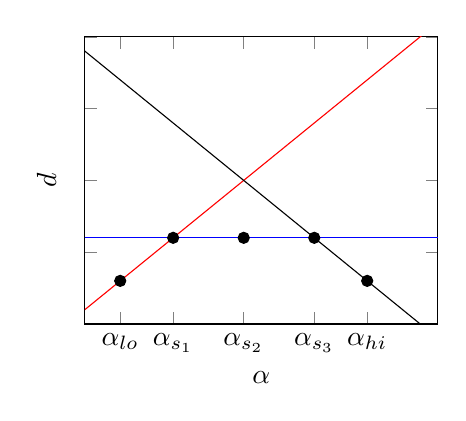
\begin{tikzpicture}
        \begin{axis}[ 
        xlabel=$\alpha$,
        ylabel={$d$},
        xmin=0.4,
        xmax=0.9,
        xtick={0.45,0.525,0.625,0.725,0.8},
        xticklabels={$\alpha_{lo}$, $\alpha_{s_1}$, $\alpha_{s_2}$, $\alpha_{s_3}$, $\alpha_{hi}$},
        width=0.5\textwidth,
        yticklabels={,,}
        ] 
        \addplot[mark=none, red] {-3+8*x}; 
        \addplot[mark=none, black] {-8*x+7};
        \addplot[mark=none, blue] {1.2};
        \addplot [only marks] table {
        0.45   0.6
        0.525  1.2
        0.625  1.2
        0.725  1.2
        0.8    0.6
        };
        \end{axis} 
    \end{tikzpicture}
    \caption{Simply calculating the split values between the start and the end value of the range $[\alpha_{lo}, \alpha_{hi}]$ will not necessarily lead to the optimal values. By doing so, the blue line (constant $d$ value) will not be considered.}
    \label{fig:notoptimal2}
\end{figure}

By calculating the split points recursively, the example in figure \ref{fig:notoptimal2} will result in the intervals $[\alpha_{lo}, \alpha_{s_1}]$, $[\alpha_{s_1}, \alpha_{s_2}]$, $[\alpha_{s_2}, \alpha_{s_3}]$ and $[\alpha_{s_3}, \alpha_{s_{hi}}]$. The optimal distance between $\alpha_{s_1}$ and $\alpha_{s_3}$ is covered now, but the results contain one unncessary interval as $\alpha_{s_2}$ still splits two intervals. The algorithm can check if older splits are still relevant, however the runtime cost to do so will be more expensive than carrying one additional interval with the same distance. We can use this knowledge and adapt algorithm \ref{alg:alphalinkage1}.

\begin{algorithm}[H]
    \KwData{input data $p_1, ..., p_N$, initial states $st$}
    \KwResult{$k$ intervals $[\alpha_0, \alpha_1], ..., [\alpha_{k-1},\alpha_k]$}
    \For{$iteration\gets1$ \KwTo $N-1$}{
        \ForEach{state $s \in st$}{%
        remove state $s$\;
        ranges $\gets$ find ranges between $s.\alpha_{lo}$ and $s.\alpha_{hi}$\;
        \ForEach{range $r \in ranges$}{%
                $cand \gets$ candidate for range\;
                $ms \gets$ merge $cand$\;
                add state $ms$ with range $r$ to the end of $st$\;
        }
      }
    }
    \caption{By calculating the split points between $\alpha_{lo}$ and $\alpha_{hi}$ recursively, we ensure that no optimal interval is left out.}
    \label{alg:alphalinkage2}
\end{algorithm}

As experimental results turn out to need a lot of memory (up to $\approx$ 20 GB for 300 points and 20,000 states), we want to adapt algorithm \ref{alg:alphalinkage2} so that it uses less memory. The memory usage scales relative to the amount of currently in-memory stored states, so the goal is to reduce these. As the amount of states is much larger than the amound of iterations, we calculate and evaluate the leave nodes of the tree and keep the alternative merges stored. This results in algorithm \ref{alg:alphalinkage3}.

\begin{algorithm}[H]
    \KwData{input data $p_1, ..., p_N$, initial states $st$}
    \KwResult{$k$ intervals $[\alpha_0, \alpha_1], ..., [\alpha_{k-1},\alpha_k]$}
    \While{$|st| > 0$}{
        \ForEach{state $s \in st$}{%
        remove state $s$\;
        \eIf{$s$ is final}{
          evaluate $s$\;
          }{
          ranges $\gets$ find ranges between $s.\alpha_{lo}$ and $s.\alpha_{hi}$\;
            \ForEach{range $r \in ranges$}{%
                    $cand \gets$ candidate for range\;
                    $ms \gets$ merge $cand$\;
                    add state $ms$ with range $r$ to the beginning of $st$\;
            }
         }
      }
    }
    \caption{Instead of calculating the nodes layerwise, this algorithm works pathwise, i.e. it goes down one path of a tree to a leaf node and evaluates it before continuing with the next split. This approach needs much less memory than the previous algorithms and has about the same runtime as shown in figure \ref{fig:performance}.}
    \label{alg:alphalinkage3}
\end{algorithm}

\begin{figure}[H]
\centering
\begin{minipage}{.45\textwidth}
  \centering
  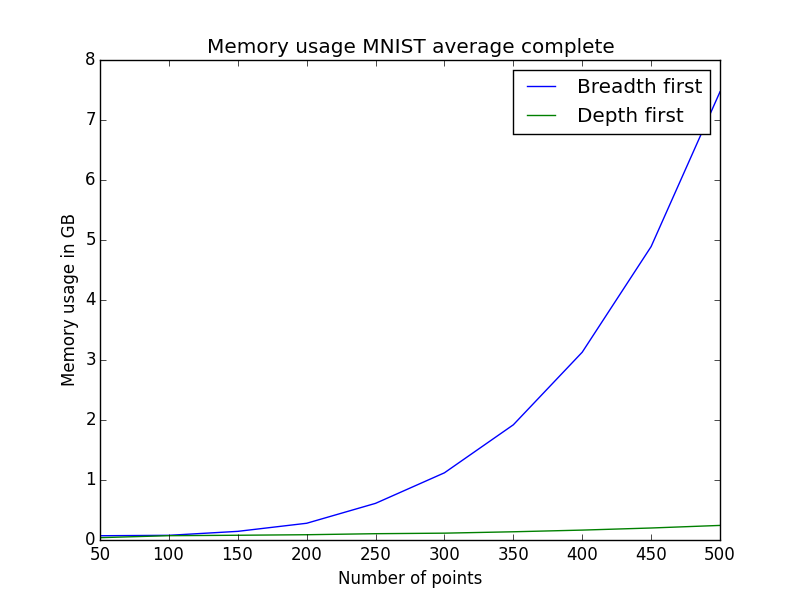
\includegraphics[width=\linewidth]{plots/memory_mnist_ac}
\end{minipage}\hfill
\begin{minipage}{.45\textwidth}
  \centering
  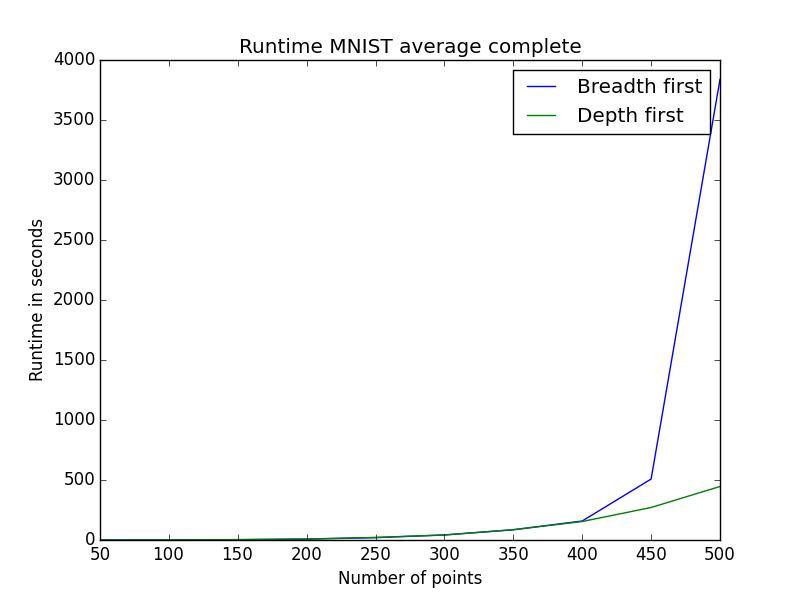
\includegraphics[width=\linewidth]{plots/runtime_mnist_ac}
\end{minipage}
\caption{The depth first implementation needs less memory and also has a better runtime compared to the breadth first implementation.}
\label{fig:performance}
\end{figure}

Instead of merging iteratively and steadily shrinking the intervals, we propose an algorithm with a geometric motivation. We are again evaluating an interval $[\alpha_{lo}, \alpha_{hi}]$, but we interprete the different merges as linear functions depending on $\alpha$. We can start by calculating the merge candidate for the start value $\alpha_{lo}$ and calculate the next intersection that will yield to the next merge. By calculating all the intersections of linear functions, we can also determine all the different intervals for the range $[\alpha_{lo}, \alpha_{hi}]$, where different merging behaviors occure. Algorithm \ref{alg:alphalinkage4} describes this procedure.

\begin{algorithm}[H]
    \KwData{input data $p_1, ..., p_N$, start value $\alpha_{lo}$, end value $\alpha_{hi}$}
    \KwResult{$k$ intervals $[\alpha_0, \alpha_1], ..., [\alpha_{k-1},\alpha_k]$}
    $\alpha \gets \alpha_{lo}$\;
    linear function $lf \gets$ get lf for alpha\;
    \While{$\alpha < \alpha_{hi}$}{
        $\alpha_{new} \gets$ calculate next split for $\alpha$\; 
        $lf \gets$ get lf for $\alpha_{new}$\;
        $\alpha \gets \alpha_{new}$
    }
    \caption{}
    \label{alg:alphalinkage4}
\end{algorithm}

\begin{figure}[H]
    \centering
    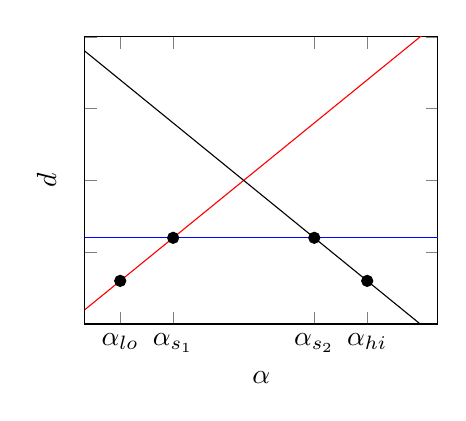
\begin{tikzpicture}
        \begin{axis}[ 
        xlabel=$\alpha$,
        ylabel={$d$},
        xmin=0.4,
        xmax=0.9,
        xtick={0.45,0.525,0.725,0.8},
        xticklabels={$\alpha_{lo}$, $\alpha_{s_1}$, $\alpha_{s_2}$, $\alpha_{hi}$},
        width=0.5\textwidth,
        yticklabels={,,}
        ] 
        \addplot[mark=none, red] {-3+8*x}; 
        \addplot[mark=none, black] {-8*x+7};
        \addplot[mark=none, blue] {1.2};
        \addplot [only marks] table {
        0.45   0.6
        0.525  1.2
        0.725  1.2
        0.8    0.6
        };
        \end{axis} 
    \end{tikzpicture}
    \caption{Simply calculating the split values between the start and the end value of the range $[\alpha_{lo}, \alpha_{hi}]$ will not necessarily lead to the optimal values. By doing so, the blue line (constant $d$ value) will not be considered.}
    \label{fig:optimal}
\end{figure}

\section{Performance Optimizations}

In order to have real-world applications, the proposed algorithms should run in an efficient way, i.e. it should not take the $\alpha$-linkage algorithms too much time to run. A first python implementation took days to run, but switching to C++ and using its advantages took down the runtime to hours. However, there are more optimization methods that we used in order to improve the runtime.

\subsection{Dynamic Programming}

One of the most time-consuming parts was the calculating of the distances. For each pair of clusters $C_i, C,j$ the distance had to be calculated for each clustering state. We optimized this by using dynamic programming and stored the distance matrices $D_{lower}$ and $D_{upper}$ for each state. The naming results from the different interpolation settings where we interpolate from one linkage distance (lower) to another linkage distance (upper), e.g. the setting in equation \ref{eq:singlecomplete} describes the interpolation from single linkage (lower) to complete linkage (upper). In this example we then store the pairwise distances for both single linkage and complete linkage and in order to find the merge candidates we have to do iterate over the distance matrices instead of calculating the distances over and over again. When we merge two clusters, we then update the distance matrices for the given state. Table \ref{dp:distances} shows an example for the pairwise distances of clusters $i$ and $j$.

\begin{table}[H]
    \centering
    \begin{tabular}{|l | l l l l l|}
    \hline
    j\textbackslash i & 0 & 1 & 2 & 3 & 4\\ \hline
    0 & 0 & 1.243 & 1.512 & 2.468 & 5.1243\\
    1 & 1.243 & 0 & 2.443 & 3.1412 & 4.443\\
    2 & 1.512 & 2.443 & 0 & 3.8988 & 6.827\\
    3 & 2.468 & 3.1412 & 3.8988 & 0 & 5.72\\
    4 & 5.1243 & 4.443 & 6.827 & 5.72 & 0\\ \hline
    \end{tabular}
    \caption{Storing the pairwise distances of all clusters avoids calculating the distances over and over again.}
    \label{dp:distances}
\end{table}

One observation that we can make is that the matrix has a lot of redundant values, because $D(i,j) = D(j,i)$. Removing these rendundant values will result in a trade-off between copying and indexing costs and will be discussed in the following section. Another optimization we can do is storing the indices of the active clusters, i.e. the clusters that can get merged. Once two clusters got merged, they cannot be merged any further, only the resulting cluster can. So we then do not have to consider the old clusters anymore and can remove them from the set of active indicies. This allows us to find the merge candidates faster as the pool of candidates gets smaller.

\subsection{Trade-Off between Copying and Indexing Costs}

Currently we can access the costs for a pair of clusters $C_i$ and $C_j$ through $D[i,j]$ or $D[i + j * width]$ for flattened matrices. These indices are very easy to calculate. In order to remove the redundant values from the distance matrix we remove all values below the diagonal as shown in table \ref{dp:distances2}.

\begin{table}[h]
    \centering
    \begin{tabular}{|l | l l l l l|}
    \hline
    j\textbackslash i & 0 & 1 & 2 & 3 & 4\\ \hline
    0 & 0 & 1.243 & 1.512 & 2.468 & 5.1243\\
    1 & \cellcolor{gray!25} & 0 & 2.443 & 3.1412 & 4.443\\
    2 & \cellcolor{gray!25} & \cellcolor{gray!25} & 0 & 3.8988 & 6.827\\
    3 & \cellcolor{gray!25} & \cellcolor{gray!25} & \cellcolor{gray!25} & 0 & 5.72\\
    4 & \cellcolor{gray!25} & \cellcolor{gray!25} & \cellcolor{gray!25} & \cellcolor{gray!25} & 0\\ \hline
    \end{tabular}
    \caption{Storing the pairwise distances of all clusters avoids calculating the distances over and over again.}
    \label{dp:distances2}
\end{table}

In addition to that we can also remove the diagonal values as they represent the distances between the same clusters and are thus always zero. This results in table \ref{dp:distances3}.

\begin{table}[H]
    \centering
    \begin{tabular}{|l | l l l l l|}
    \hline
    j\textbackslash i & 0 & 1 & 2 & 3 & 4\\ \hline
    0 & \cellcolor{gray!25} & 1.243 & 1.512 & 2.468 & 5.1243\\
    1 & \cellcolor{gray!25} & \cellcolor{gray!25} & 2.443 & 3.1412 & 4.443\\
    2 & \cellcolor{gray!25} & \cellcolor{gray!25} & \cellcolor{gray!25} & 3.8988 & 6.827\\
    3 & \cellcolor{gray!25} & \cellcolor{gray!25} & \cellcolor{gray!25} & \cellcolor{gray!25} & 5.72\\
    4 & \cellcolor{gray!25} & \cellcolor{gray!25} & \cellcolor{gray!25} & \cellcolor{gray!25} & \cellcolor{gray!25} \\ \hline
    \end{tabular}
    \caption{Storing the pairwise distances of all clusters avoids calculating the distances over and over again.}
    \label{dp:distances3}
\end{table}

The matrices are now smaller, so they need less memory. In the example, we changed a matrix of the size $25$ to a matrix of the size $10$. In general a matrix of the size $n$x$n$ will be compressed to a matrix of the size $\frac{n^2-n}{2}$. The lower amount of needed memory also results in less copying costs that will lead to a better runtime. However, the indexing is not as easy anymore. For easier storage, we again work with flattened matrices, the indexing for the resulting list is shown in equation \ref{eq:indexing}.

\begin{equation}
    \begin{aligned}
        index(i,j) = \frac{width * (width - 1)}{2} - \frac{(width - j) * (width - j - 1)}{2} + i - j - 1
    \end{aligned}
    \label{eq:indexing}
\end{equation}

Calculating this index in a nested loop is very expensive, however we calculate the part that does not depend on $i$ in the outer loop and thus only need to add $i$ in the inner loop. This does not only yield to a lower memory usage of $\approx 30\%$, but also increases the runtime by TODO.

\todo[inline]{runtime improvement factor}

\subsection{Implementation-specific Optimizations}

In order to optimize the implementation even further, we will have a look into the implementation. One optimization that already was briefly described is the flatterning of the matrices, so the resulting list will be one-dimensional and can be iterated easier and faster.\\

Another observation is that copy operations are computationally expensive, so we avoid them as much as possible. In the described algorithms (\ref{alg:alphalinkage1}, \ref{alg:alphalinkage2} and \ref{alg:alphalinkage3}) we removed a state from the list of states and added other states. In an optimized way, we do not remove the state and just overwrite the state with the resulting state. Once there are splits in the current interval, the state gets overwritten and additional states get added to the list.\\

We can also optimize the way of updating the distance matrices. Instead of adding new clusters there for a merge of clusters $i$ and $j$ we update the distances of $i$ to all active clusters with the distances of the resulting cluster. The distances of the cluster $j$ will not be considered for merges anymore as the index $j$ gets removed from the active indices. This has the advantage that the size of the distance matrices will not increase after merges.\\

Also, the data types make an important contribution to the memory usage. Instead of using double precision floating point values, single precision is enough to clearly identify and separate all the resulting intervals. Same goes for the distances as we only need the minimum and maximum distances, that are not effected by loss of precision. To store the indices of the clusters, we know that they will not exceed $2^{16}$, so they can be store as half precision values.

\chapter{Optimizing the Metric}
\label{sec:beta}

In a similar fashion as described in section \ref{chapter:alphalinkage}, this sections aims to find an optimized feature representation that is a linear combination of several metrics. For instance, images can have a 2-dimensional pixel representation and a text describing each image. Combining these features for clustering tasks can be problematic as it is not trivial how the optimal weight between these features should be. Does a word describe more than a fragment of the image, are the features equally important or does the pixel image lead to better clusterings? With $\beta$-linkage we provide a framework based on $\alpha$-linkage that calculates different merges based on linear combinations of representations and leads to optimized clusterings.

\begin{figure}[h]
    \centering
    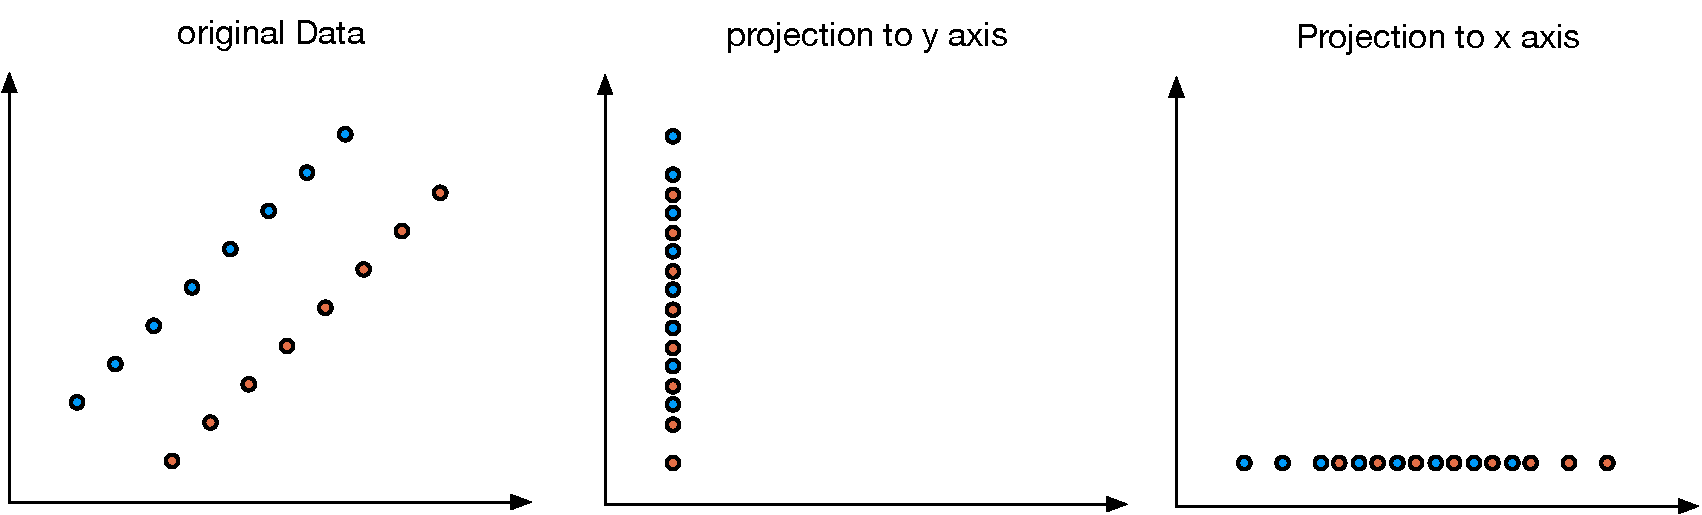
\includegraphics[width=0.7\textwidth]{images/ExampleDataset}
    \caption{Combining several metrics seems often natural and can lead to improved results as in this example where we project a dataset on the $x_1$- and the $x_2$-axis.}
    \label{fig:metrics}
\end{figure}

For instance, figure \ref{fig:metrics} shows a set of points that might be put in clusters easily. However, if you only look at the distance regarding the $x_1$-axis or the $x_2$-axis, a perfect clustering will no longer be possible, because each of the axes does not describe the spatial correlation anymore. This example is selected on purpose to motivate the following experiments where we learn optimal combinations of different metrics.\\ 

To interpolate between $d_0$ and $d_1$, we use the same interpolation as discussed in section \ref{chapter:alphalinkage}. We use a parameter $\beta \in [0,1]$ and weight the metrics as shown below.

\begin{align}
d_\beta(x,x') &= (1 - \beta) \cdot d_0(x,x') + \beta \cdot d_1(x,x') \nonumber \\
&= d_0(x,x') + \beta \cdot (d_1(x,x') - d_0(x,x'))
\label{eq:betalinkage}
\end{align}

We can then compute all possible discontinuities by comparing the distances of given clusters $(x, x')$ and $(y, y')$. As $d_\beta(x,x')$ is a linear function depending on $\beta$ (see equation \ref{eq:betalinkage}), we can compute all discontinuities by solving the following equation.

\begin{equation*}
    \begin{aligned}
      \begin{gathered}
        d_\beta(x,x') = d_\beta(y,y')\\
        (1 - \beta) \cdot d_0(x,x') + \beta \cdot d_1(x,x') = (1 - \beta) \cdot d_0(y,y') + \beta \cdot d_1(y,y')\\
        d_0(x,x') - \beta \cdot d_0(x,x') + \beta \cdot d_1(x,x') = d_0(y,y') - \beta \cdot d_0(y,y') + \beta \cdot d_1(y,y')\\
        \beta \cdot (- d_0(x,x') + d_1(x,x') + d_0(y,y') - d_1(y,y')) = - d_0(x,x') + d_0(y,y')\\
        \beta = \frac{- d_0(x,x') + d_0(y,y')}{- d_0(x,x') + d_1(x,x') + d_0(y,y') - d_1(y,y')}
        \label{eq:discont}
      \end{gathered}
    \end{aligned}
\end{equation*}
As we know that the function $d_\beta$ is a linear function depending on $\beta$ and we showed that all discontinuities depend on four points, we know that there are at most $O(n^4)$ well-defined intervals $\mathcal{I}_i \in [0,1]$ for any clustering instance $S$, i.e. in any interval $\mathcal{I}_i$ the algorithm will merge the same two points. In order to efficiently calculate and evaluate all resulting cluster trees, we use an algorithm similar to algorithm \ref{alg:alphalinkage4}, but adapted to $\beta$-linkage.

\begin{algorithm}
\textbf{Input:} Metrics $\dZero$ and $\dOne$, parameter $\beta \in [0,1]$, and clustering instance $S = \{x_1, \dots, x_n\}$.
\begin{enumerate}[nosep, leftmargin=*]
\item Let $\mathcal{N} = \{\leaf(x_1), \dots, \leaf(x_n)\}$ be the initial set of nodes (one leaf per point).
\item While $|\mathcal{N}| > 1$
\begin{enumerate}[nosep, leftmargin=*]
  \item Let $A, B \in \mathcal{N}$ be the clusters in $\mathcal{N}$ minimizing $\max_{a \in A, b \in B} \dbeta(a, b)$.
  \item Remove nodes $A$ and $B$ from $\mathcal{N}$ and add $\node(A,B)$ to $\mathcal{N}$.
\end{enumerate}
\item Return the cluster tree (the only element of $\mathcal{N}$).
\end{enumerate}
\caption{$\beta$-linkage Clustering}
\label{alg:betalinkage}
\end{algorithm}

A slight adaption that we need is to normalize the features such that for $\beta = 0.5$ we equally weight both distance matrices. We achieve this by dividing the features $f_1, \dots, f_k$ through the maximum value $f_{max}$. In this way, we scale the features into $[0,1]$ and do not lose the proportions as it would happen when e.g.\ using a min-max-scaler.

% \chapter{$\alpha$-$\beta$-Linkage}

\section{Bilinear Interpolation between three different linkage strategies}

\section{Adapted Algorithm}

\chapter{Experimental Setup}

This work evaluates the proposed algorithms for image and text data. This chapter describes the used datasets, the evaluation methods and the experimental setups.

\section{Datasets}
\label{sec:datasets}

\subsection{Never Ending Language Learner data}

The Never Ending Language Learner (NELL) is a learning agent that reads the web, extracts data and verfies beliefs \cite{Mitchell:2015:NL:2886521.2886641}\cite{Mitchell:2018:NL:3210350.3191513}. NELL for example knows that "Pittsburgh" is located in "Pennsylvania". These beliefs represent different noun-phrases such as "Pittsburgh" and "Pennsylvania". The noun-phrases belong to certain categories. "Pittsburgh" is a "City" and "Pennsylvania" is a "State". These subcategories both belong to the main category "Geopolitical Location". While there are already different subcategories, the goal for a hierarchical clustering algorithm here is to extract new useful subcategories.

The used dataset, extracted web-information by NELL, contains 32 different main categories, such as "Animal", "Location" or "Person". Each of these consists of up to 250 different entities that belong to different subcategories. Examplary entites for the category "Animal" are "Otter", "Squirrel" or "Wolf". 

This thesis shows in chapter \ref{sec:results} the learned subcategories.

\subsection{MNIST handwritten digits}

The MNIST handwritten digit database contains images of the handwritten digits from zero to nine \cite{lecun-mnisthandwrittendigit-2010}. Samples of these images are shown in figure \ref{fig:mnist} Its training set contains a total of 60,000 images, where each image is represented as a 784-dimensional vector corresponding to a greyscale image with 28x28 pixels.

\begin{figure}[h]
    \centering
    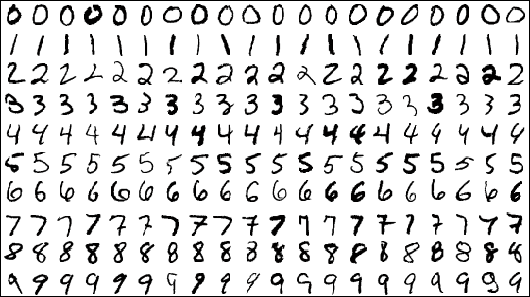
\includegraphics[width=0.7\textwidth]{images/mnist}
    \caption{The MNIST handwritten digits database contains 60,000 greyscale images of handwritten digits ranging from zero to nine. These samples show ten randomly drawn samples for each label represented as a 28x28 pixel image \cite{lecun-mnisthandwrittendigit-2010}.}
    \label{fig:mnist}
\end{figure}

The goal of clustering MNIST images is to find an unsupervised learning method that can distinguish between greyscale images. In addition, we can define various clustering tasks where we pick a subsample of the ten labels and then try to transfer the results to other subsamples. For example, we first cluster images labeled as zero, one, two, three or four and later apply the knowledge the learned gained for clustering images labeled as five, six, seven, eight or nine. Theses types of experiments allow high-level transfer learning if we define several different clustering tasks, e.g. for five different labels there are $10 \choose 5$ $= 252$ different combinations of labels.

Another obsevation that results from hierarchical clustering is the similarity of different labels, i.e. which labels are likely to get clustered together.

\subsection{CIFAR-10}

Another image dataset this thesis uses for evaluation is the CIFAR-10 dataset that contains 60,000 RGB images of ten different categories \cite{Krizhevsky2009LearningML}. Each image consists of 32x32 pixels and is thus represented as a 3072-dimensional vector (32x32x3). The categories and ten random images from each are shown in figure \ref{fig:cifar10}.

\begin{figure}[h]
    \centering
    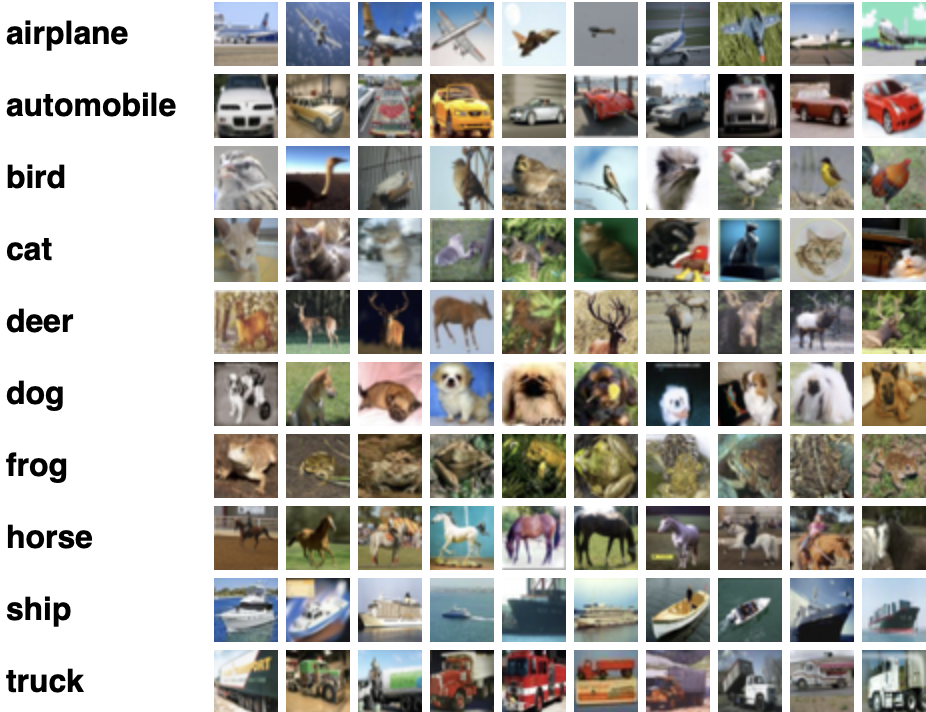
\includegraphics[width=0.7\textwidth]{images/cifar10}
    \caption{The CIFAR-10  database contains 60,000 RGB images of the ten shown different classes. These samples show ten randomly drawn samples for each label represented as a 32x32 pixel image \cite{Krizhevsky2009LearningML}.}
    \label{fig:cifar10}
\end{figure}

As the amount of images and the amount of classes is equal to the ones in the MNIST database, we can also try similar experiments. The main difference is that the images consist of RGB pixels instead of greyscale values.

\subsection{CIFAR-100}

The CIFAR-100 dataset contains similar images, but instead of 6,000 images each for 10 classes, it consists of 600 images each for 100 classes. The classes are divided into 20 superclasses each containing five subclasses. Examples of superclasses and corresponding subclasses are shown in table \ref{table:cifar100data}. 

\begin{table}[h]
    \centering
    \begin{tabular}{|l|l|}
    \hline
    superclass      & subclasses                                  \\ \hline
    aquatic mammals & beaver, dolphin, otter, seal, whale         \\
    fish            & aquarium fish, flatfish, ray, shark, trout  \\
    flowers         & orchids, poppies, roses, sunflowers, tulips \\
    people          & baby, boy, girl, man, woman                 \\ 
    reptiles        & crocodile, dinosaur, lizard, snake, turtle  \\ \hline               
    \end{tabular}
    \caption{The CIFAR-100 dataset contains 20 different superclasses, each with five different subclasses leading to 100 classes overall. The images are represented in the same way as in the CIFAR-10 dataset, i.e. by a 3072-dimensional vector \cite{Krizhevsky2009LearningML}.}
    \label{table:cifar100data}
\end{table}

Having superclasses and subclasses allows clustering between different subclasses within a superclass and also between different superclasses. This allows more experiments than for the CIFAR10 data.

\section{Cost functions}

In order to evaluate the quality of a clustering, we need some kind of cost function that compares the generated clustering $C_1,...,C_k$ with the target clustering $C_1^*, ..., C_k^*$. One method to compare them is the majority distance as shown in equation \ref{eq:majoritydistance} where $n$ ist the number of sampled points.

\begin{equation}
    \begin{aligned}
        cost_{majority}(C_{1:k}, C_{1:k}^*) = \frac{1}{n} \sum\limits_{i=1}^{k} (\|C_i\| - \max\limits_j \|C_i \cap C_j^*\|)
    \end{aligned}
    \label{eq:majoritydistance}
\end{equation}

Another way to compare two clusterings in by using the hamming distance between the generated and the target clusterings defined as shown in figure \ref{eq:hammingdistance}.

\begin{equation}
    \begin{aligned}
        cost_{hamming}(C_{1:k}, C_{1:k}^*) = 
    \end{aligned}
    \label{eq:hammingdistance}
\end{equation}

However, the hamming distance consists of an assignment problem to find the optimal matching $\sigma$ between the generated clusters and the target clusters. Table \ref{table:matching} shows how such a matching can look like.

\begin{table}[h]
    \centering
    \begin{tabular}{|l | l l l l l|}
    \hline
    j\textbackslash i & 1 & 2 & 3 & 4 & 5\\ \hline
    1 & 20 & \cellcolor{blue!25}15 & 30 & 50 & 40\\
    2 & 80 & 10 & \cellcolor{blue!25}15 & 20 & 30\\
    3 & \cellcolor{blue!25}20 & 30 & 50 & 80 & 60\\
    4 & 30 & 50 & 40 & \cellcolor{blue!25}20 & 10\\
    5 & 20 & 30 & 40 & 50 & \cellcolor{blue!25}25\\ \hline
    \end{tabular}
    \caption{In order to calculate the hamming distance between two clusterings, we have to calculate the optimal mapping that results in lowest distance for these two clusterings. For random distances between clusterings $C_1^i, ..., C_k^i$ and $C_1^j, ..., C_k^j$ we can calculate the optimal mapping (blue highlighted cells) in a brute force way or more efficiently with the hungarian method \cite{kuhn1955hungarian}\cite{munkres1957algorithms}.}
    \label{table:matching}
\end{table}

While solving the assignment with a brute force strategy would result in $O(n!)$ complexity, Harold Kuhn introduced the hungarian method to solve the problem in $O(n^4)$ complexity \cite{kuhn1955hungarian}. Later on, James Munkred modified the algorithm to $O(n^3)$ complexity \cite{munkres1957algorithms}. A detailed explanation of the hungarian method is included in appendix \ref{sec:hungarian}.

\section{Experiments}

In order to find new subclusters for the NELL data, we cluster each of the 32 main categories seperately. This results in 32 different clustering tasks, where we compare the results of each clustering task with the target labels using the majority distance function. We will receive a cost function $cost(\alpha)$, that shows us for which value of $\alpha$ the resulting clusterings are good, for each category. By averaging all cost functions, we know for which values of $\alpha$ the $\alpha$-linkage performs well in general. Beside having a value of $\alpha$ that can be used for other clustering tasks, the experiments also give different representation levels of clusters that are discussed in section \ref{sec:results}.

To cluster the image data, we set up $10 \choose 5$ $= 252$ different experiments by selecting all combinations of five out of the ten labels. In order to do so in efficient time, we subsample the dataset to 60 points for each label, so one experiment will cluster 300 points. By having a fixed set of point, we can show that a certain value of $\alpha$ will lead to good results for the subsampled data. We will use this kind of experiments for all in section \ref{sec:datasets} mentioned image datasets where all RGB-channels are treated equally for colored images.

In addition to these experiments, we will try to cluster as diverse as possible superclasses of the CIFAR100 dataset by manually picking the five superclasses fish, flowers, household furniture, people and vehicles 1. For each superclass we pick one subclass and evaluate the results for all $5 *$ $5 \choose 1$ $= 25$ different combinations of subclasses. In addition to the experiments with $k = 5$ clusters, we compare these results to the results for picking two different subclasses of each superclass ($5 *$ $5 \choose 2$ $= 50$ different experiments) resulting in $k = 10$ clusters and also for picking three different subclasses ($5 *$ $5 \choose 3$ $= 50$ different experiments) resulting in $k = 15$ clusters.

In comparison to picking as diverse as possible superclasses, we also evaluate the performance for as similar as possible subclasses. Similar subclasses are already given in the dataset through the subclasses within one superclass. We then evaluate the majority and the hamming cost for each superclass and again average the cost over all 20 superclasses to evaluate an optimal value for the parameter $\alpha$.

The results of these experiments are discussed in the following section \ref{sec:results}. % Experimental Setup

\chapter{Experimental Results and Discussion}
\label{sec:results}

\todo[inline]{Update plots.}
\todo[inline]{More results.}

We evaluated the in chapter \ref{chapter:alphalinkage} proposed algorithms with the in chapter \ref{chapter:datasets} discussed datasets aiming to find new subcategories for the text data and to generate better clusterings overall. The quality of the clusterings was calculated with the in chapter \ref{chapter:costfunctions} explained cost functions.

\section{Algorithm Selection}

In general we evaluate two different types of experiments that apply for most of the datasets. Only for the synthetic dataset, we evaluate the data distribution shown in figure \ref{fig:disksrings}.

\paragraph{Batch Data Experiments.} In the first one, we evaluate certain data batches, i.e. we subsample the $n$-th set of points in sorted order for each of the target classes. To generalize the experiments for larger datasets, we average over multiple batches. In our experiments, we evaluate all distinct combinations of $k$ classes, e.g. for multiple datasets we have 10 target classes and use 5 labels for our experiments, i.e. we evaluate all $10 \choose 5$ combinations to cover all possible label subsets.

\paragraph{Randomized Experiments.} In the other setting, we follow \cite{NIPS2016_6385} and \cite{pmlr-v70-finn17a}. We select the points for certain classes by random. Averaging over a large number of clustering instances allows us to cover a major fraction of the dataset. To clusters a subset of the target classes, we also select the classes by random. Overall, in case both experimental settings agree, we know that the results are generalized well for the underlying data distribution.

\paragraph{Synthetic Experiments.} Here we generated 1000 clustering instances by random given the data distribution shown in section \ref{chapter:datasets}, i.e. all instances contain four classes, two rings and two disks. In figure \ref{fig:syntheticexperiments} we observe that all three linkage strategies perform very similarly. Only single linkage does slightly better with an error below $25\%$ while both average and complete linkage are above $25\%$. Interpolating between single and linkage (a) leads to significantly lower errors, where interpolating between average and complete linkage (b) does not lead to improvements. As this example motivates interpolating between single and complete linkage, we elaborate this setting further.

\begin{figure}[H]
\centering
\begin{minipage}{.45\textwidth}
  \centering
  \subcaptionbox{SC.}
  {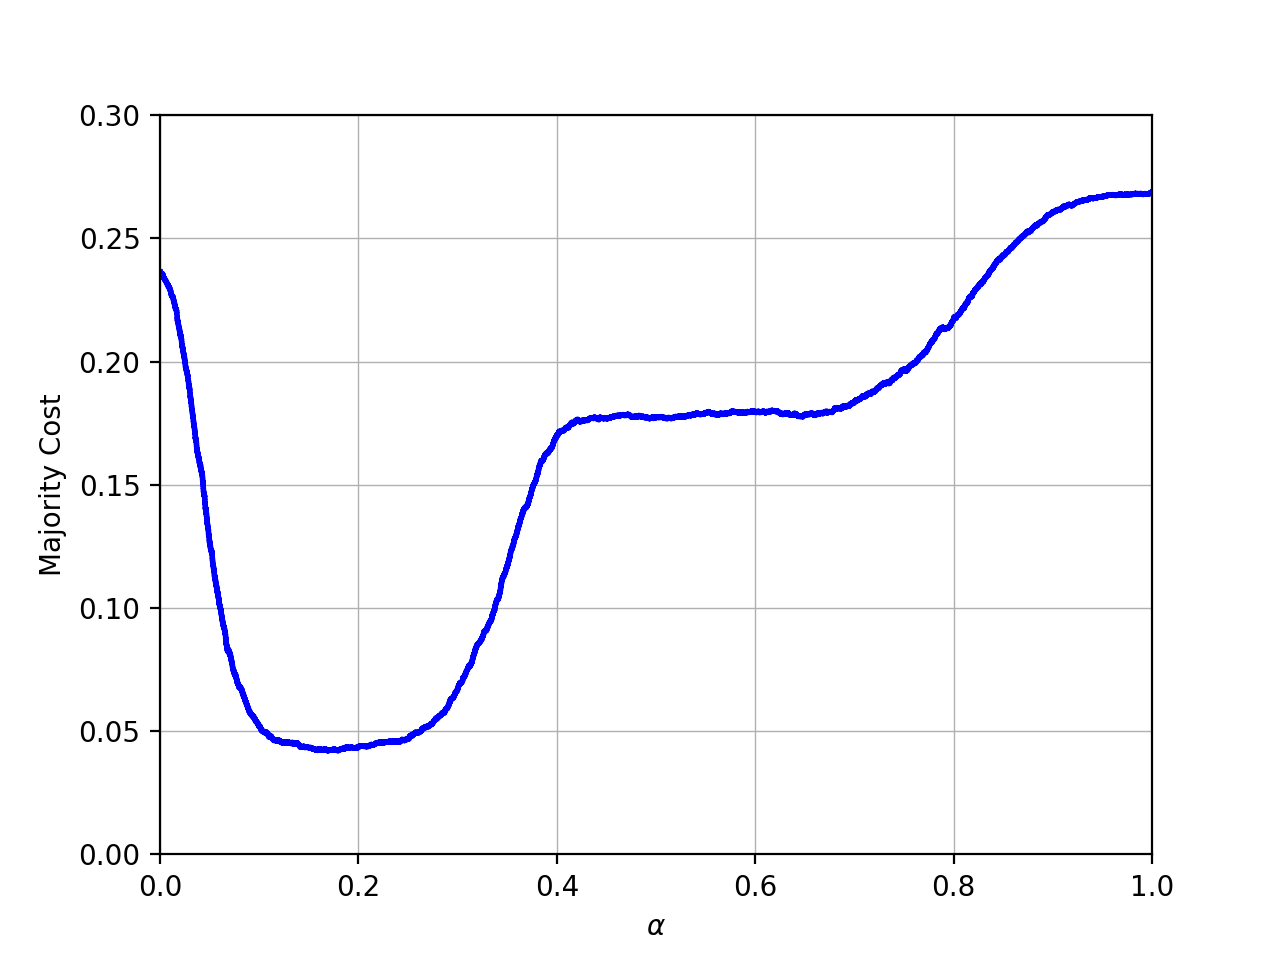
\includegraphics[width=\linewidth]{plots/ringsanddiskssc}}
\end{minipage}\quad
\begin{minipage}{.45\textwidth}
  \centering
  \subcaptionbox{AC.}
  {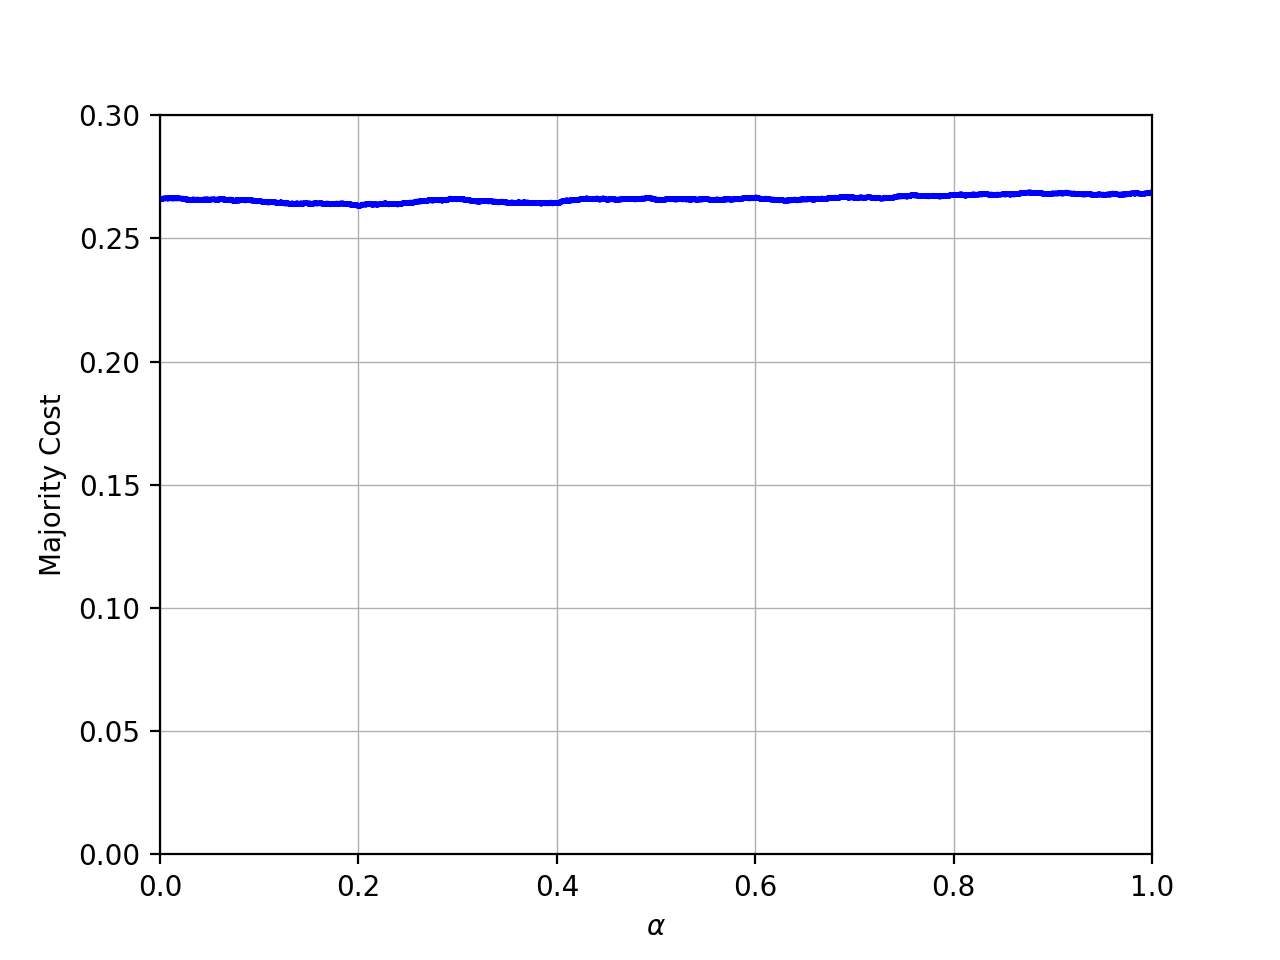
\includegraphics[width=\linewidth]{plots/ringsanddisksac}}
\end{minipage}
\caption{%
  %
  }
  %
\label{fig:syntheticexperiments}
\end{figure}

\paragraph{NELL Experiments.} In order to find new subclusters for the NELL data, we cluster each of the 32 main categories seperately. This results in 32 different clustering tasks, where we compare the results of each clustering task with the target labels using the majority distance function. We will receive a cost function $cost(\alpha)$, that shows us for which value of $\alpha$ the resulting clusterings are good, for each category. By averaging all cost functions, we know for which values of $\alpha$ the $\alpha$-linkage performs well in general. Beside having a value of $\alpha$ that can be used for other clustering tasks, the experiments also give different representation levels of clusters that are discussed in section. First, we started evaluating all tasks with a maximum of 250 points per task. Figure \ref{fig:nellresults} shows the result for all three different interpolation strategies.

\begin{figure}[h]
\centering
\begin{minipage}{.3\textwidth}
  \centering
  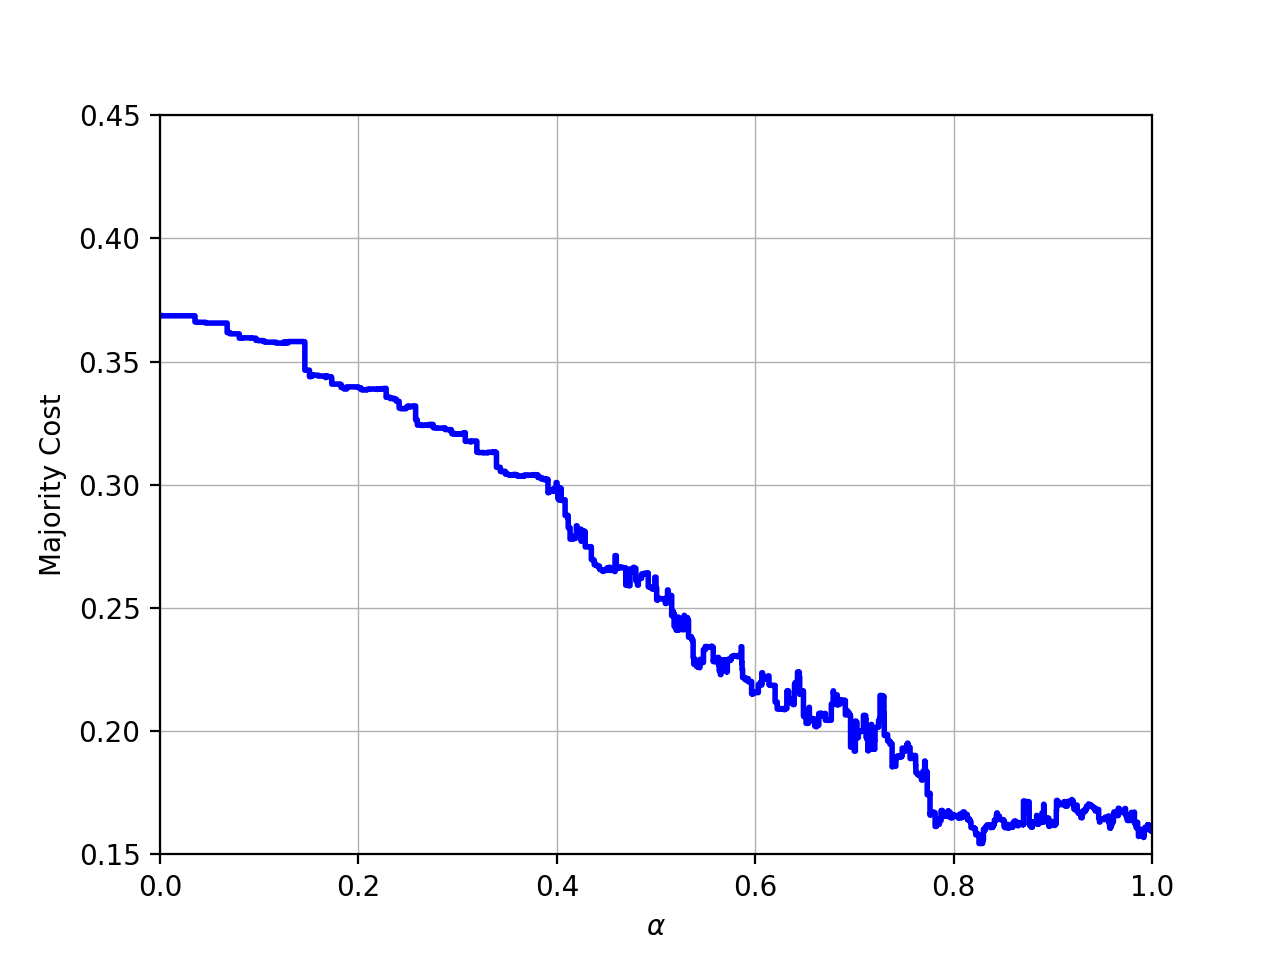
\includegraphics[width=\linewidth]{plots/nell_sc}
\end{minipage}
\begin{minipage}{.3\textwidth}
  \centering
  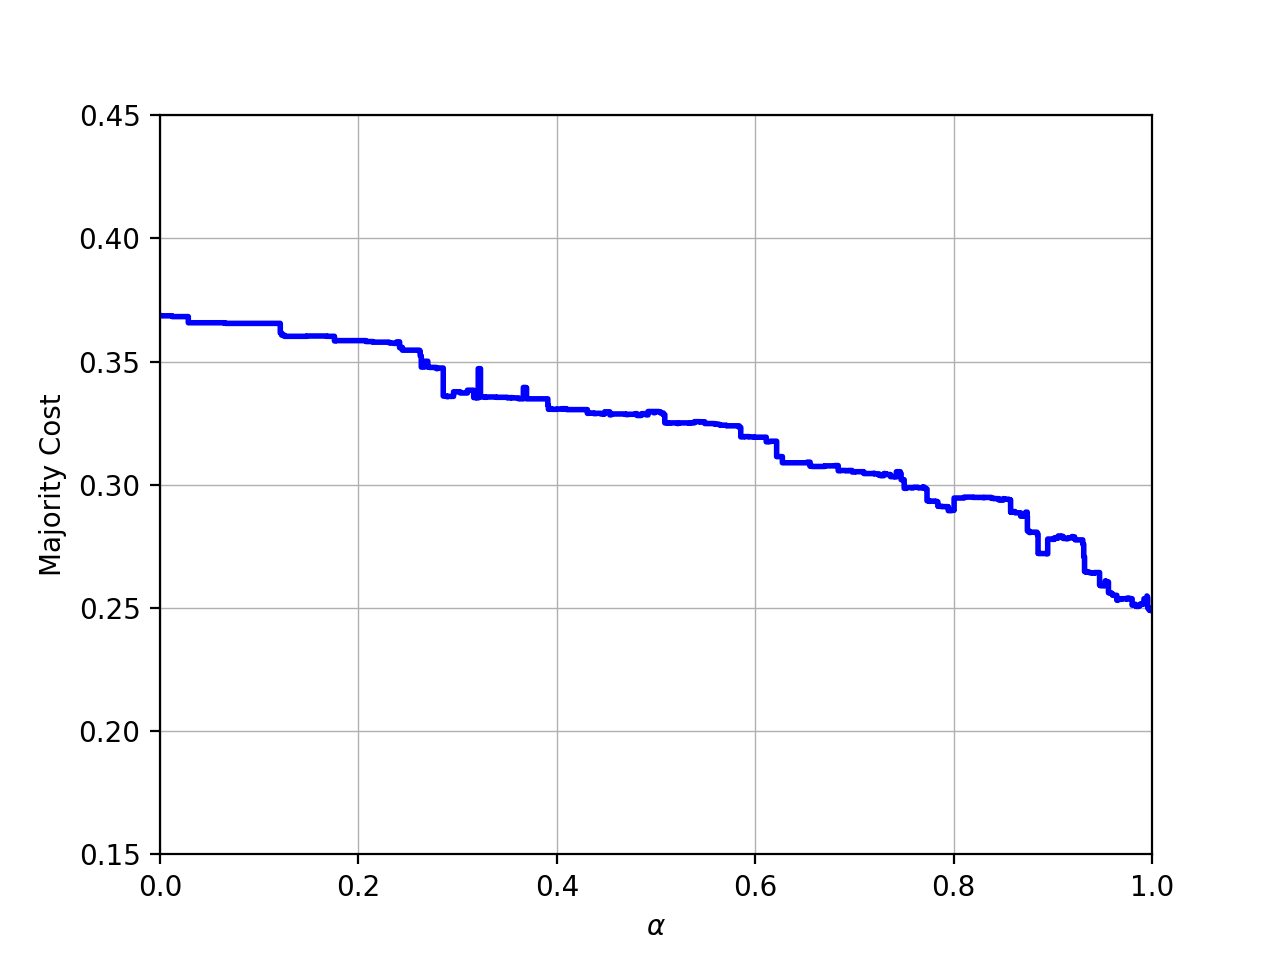
\includegraphics[width=\linewidth]{plots/nell_sa}
\end{minipage}
\begin{minipage}{.3\textwidth}
  \centering
  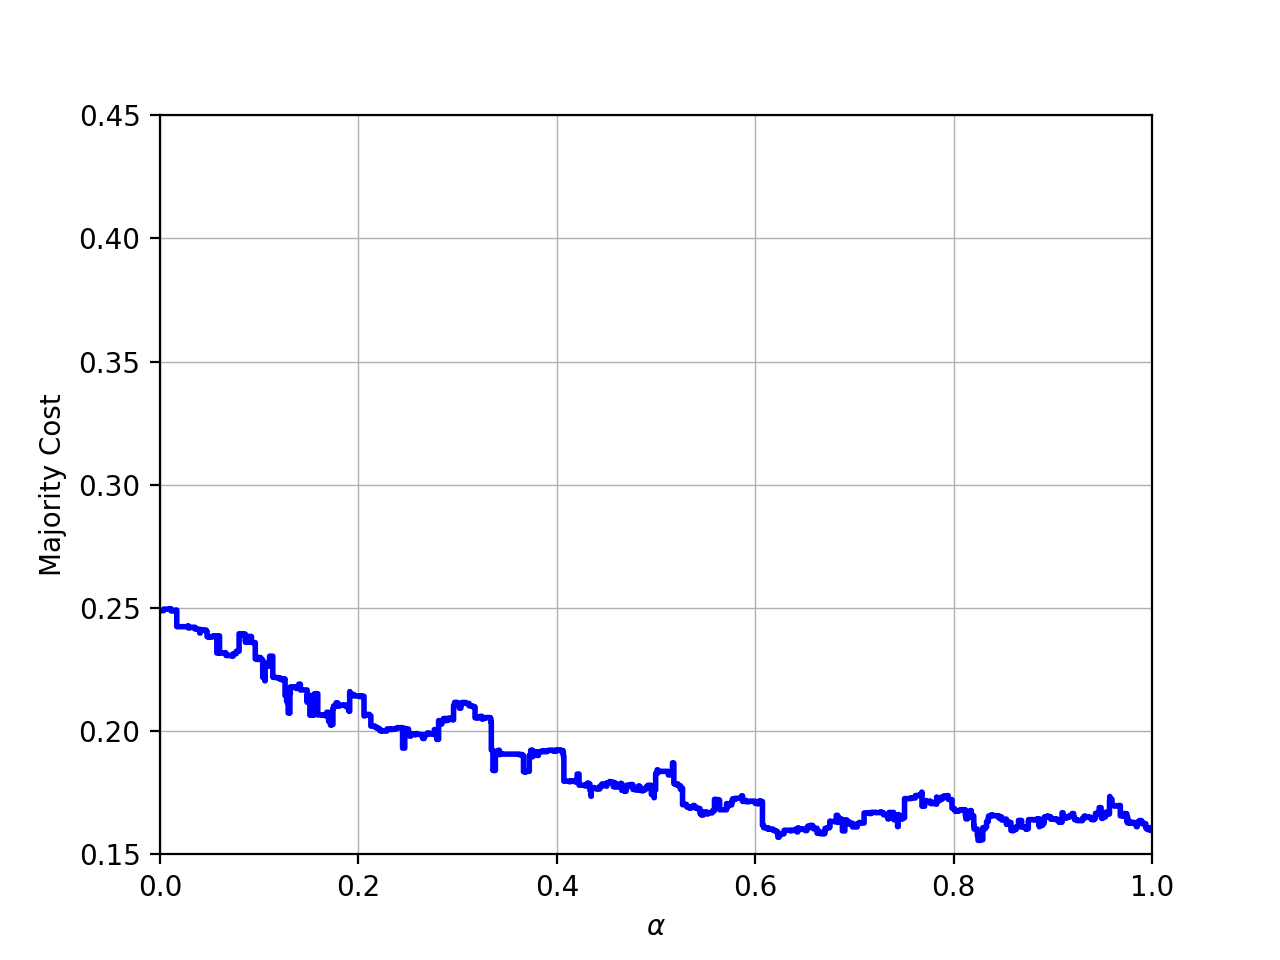
\includegraphics[width=\linewidth]{plots/nell_ac}
\end{minipage}
\caption{$\alpha$-linkage using 250 points for each clustering instance gives minor improvements for the NELL data when clustering between single and complete (left) and average and complete linkage (right). As complete linkage performs best of our input strategies, interpolating between single and average linkage (middle) does not lead to improvements.}
\label{fig:nellresults}
\end{figure}

We see minor improvements when clustering between single and complete and average and complete linkage. On the other hand, interpolating between single and average linkage did not lead to any improvement. In order to evaluate the results further, we have a closer look at the curves and see that the overall improvement we get is $0.53\%$, a reduction from $15.9725\%$ (complete linkage) to $15.4422\%$ ($\alpha_{SC}(0.826)$) as shown in table \ref{table:nellresults}. An interesting observation is that while single linkage performs very poor overall, interpolating between single and complete linkage gives a better improvement than interpolating between average and complete linkage. To evaluate these experiments we are using the Majority Distance, as for such a large number of target clusters calculating the Hamming distance is not efficient. 

\begin{table}[h]
    \centering
    \begin{tabular}{|l | l|}
    \hline
    Strategy & Majority Cost\\ \hline
    Single Linkage & 0.36871\\
    Average Linkage & 0.248913\\
    Complete Linkage & 0.159725\\
    \cellcolor{green!50}$\alpha_{SC}(0.826)$ & \cellcolor{green!50}0.154422\\
    $\alpha_{AC}(0.826)$ & 0.155697\\\hline
    \end{tabular}
    \caption{Our proposed algorithm reduces the NELL cost by $\Delta cost = 0.53\%$ when using a maximum of 250 points for each class.}
    \label{table:nellresults}
\end{table}

As the algorithm became a lot more efficient during this work, we scaled up the algorithms to use 1,000 instead of 250 points per class. Figure \ref{fig:nellresults1000} shows that in general the error is slightly higher. This is because our experiments contain more different classes. Overall, we again see slight improvements that are shown in table \ref{table:nell1000}. Compared to the previous experiments, the improvements were a bit bigger ($1.2078\%$ leading to an error of $16.6742\%$), however the overall curves look very similar. In this setting, we also evaluated the parameter advising for the first 10 parameters $\alpha^*$ (see figure \ref{fig:nell1000top10}).

\begin{figure}[h]
\centering
\begin{minipage}{.45\textwidth}
  \centering
  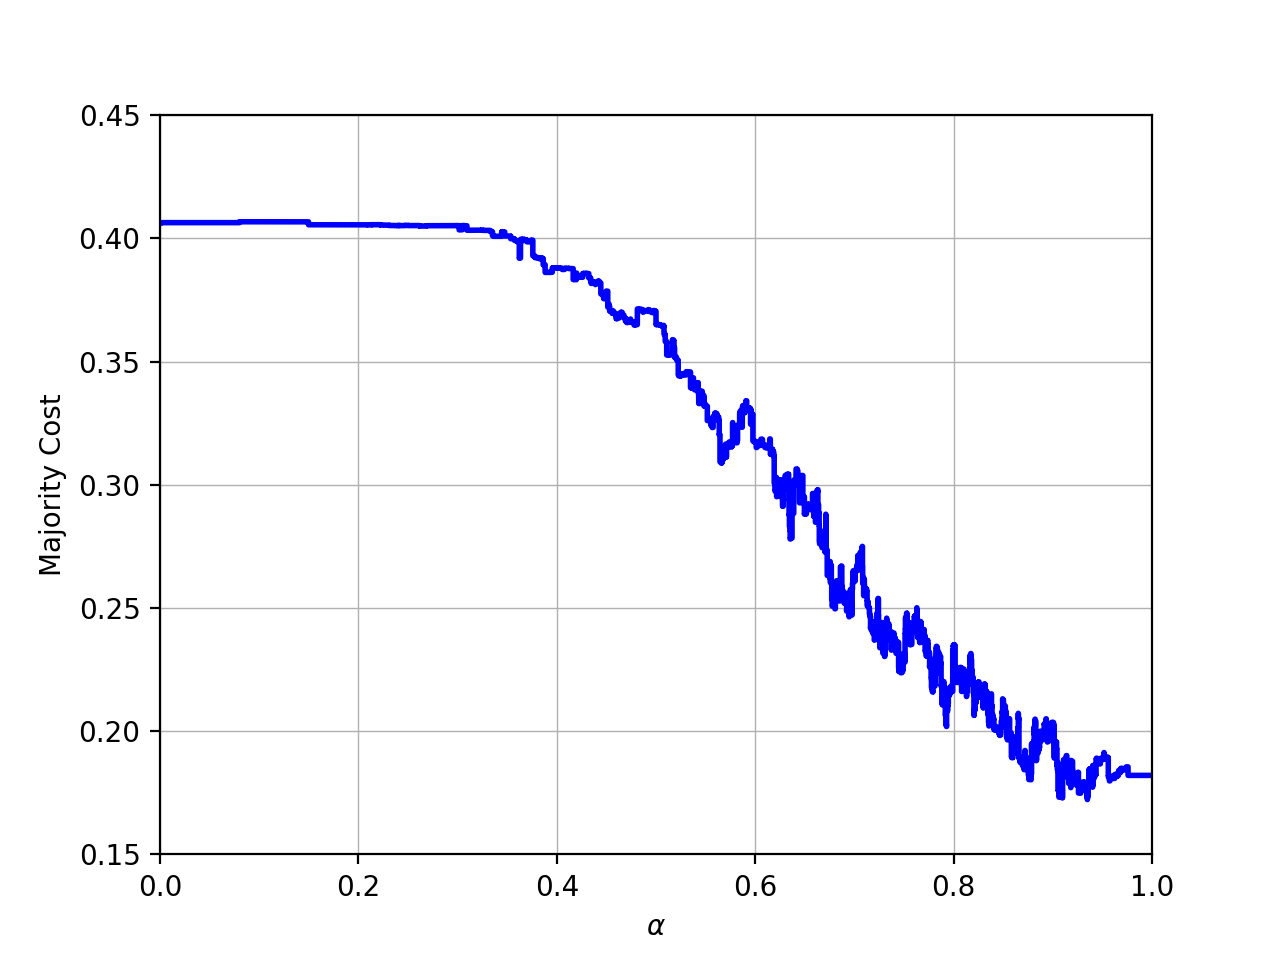
\includegraphics[width=\linewidth]{plots/nell_sc_1000}
\end{minipage}
\begin{minipage}{.45\textwidth}
  \centering
  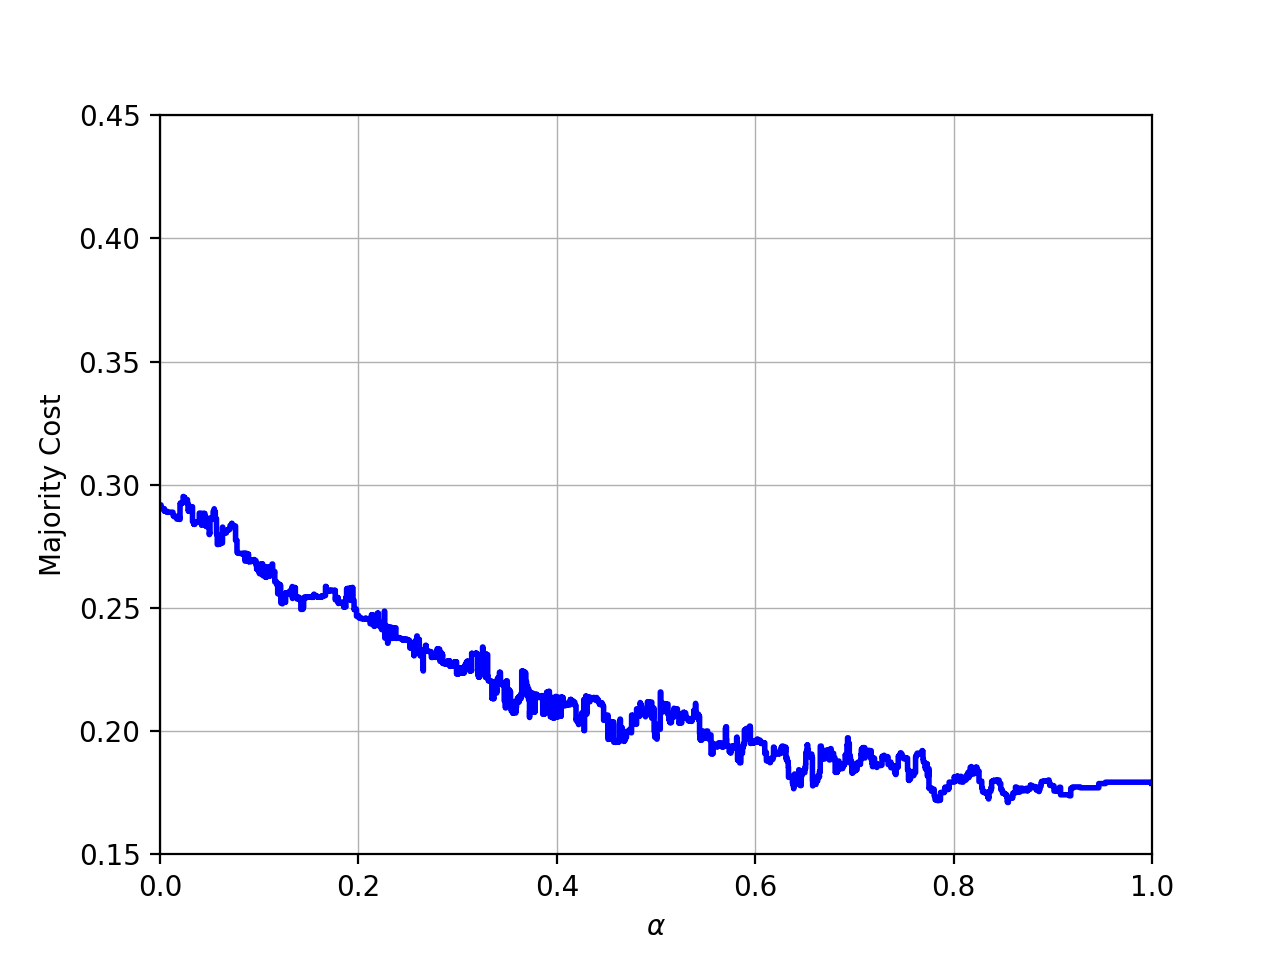
\includegraphics[width=\linewidth]{plots/nell_ac_1000}
\end{minipage}
\caption{$\alpha$-linkage using 1000 points for each clustering instance gives minor improvements for the NELL data when clustering between single and complete (left) and average and complete linkage (right).}
\label{fig:nellresults1000}
\end{figure}

\begin{table}[h]
    \centering
    \begin{tabular}{|l | l|}
    \hline
    Strategy & Majority Cost\\ \hline
    Single Linkage & 0.36871\\
    Average Linkage & 0.291202\\
    Complete Linkage & 0.17882\\
    \cellcolor{green!50}$\alpha_{SC}(0.918)$ & \cellcolor{green!50}0.166742\\
    $\alpha_{AC}(0.855)$ & 0.171083\\\hline
    \end{tabular}
    \caption{Our proposed algorithm reduces the NELL cost by $\Delta cost = 1.2078\%$ when using a maximum of 1000 points for each class.}
    \label{table:nell1000}
\end{table}

\begin{figure}[H]
\centering
\begin{minipage}{.45\textwidth}
  \centering
  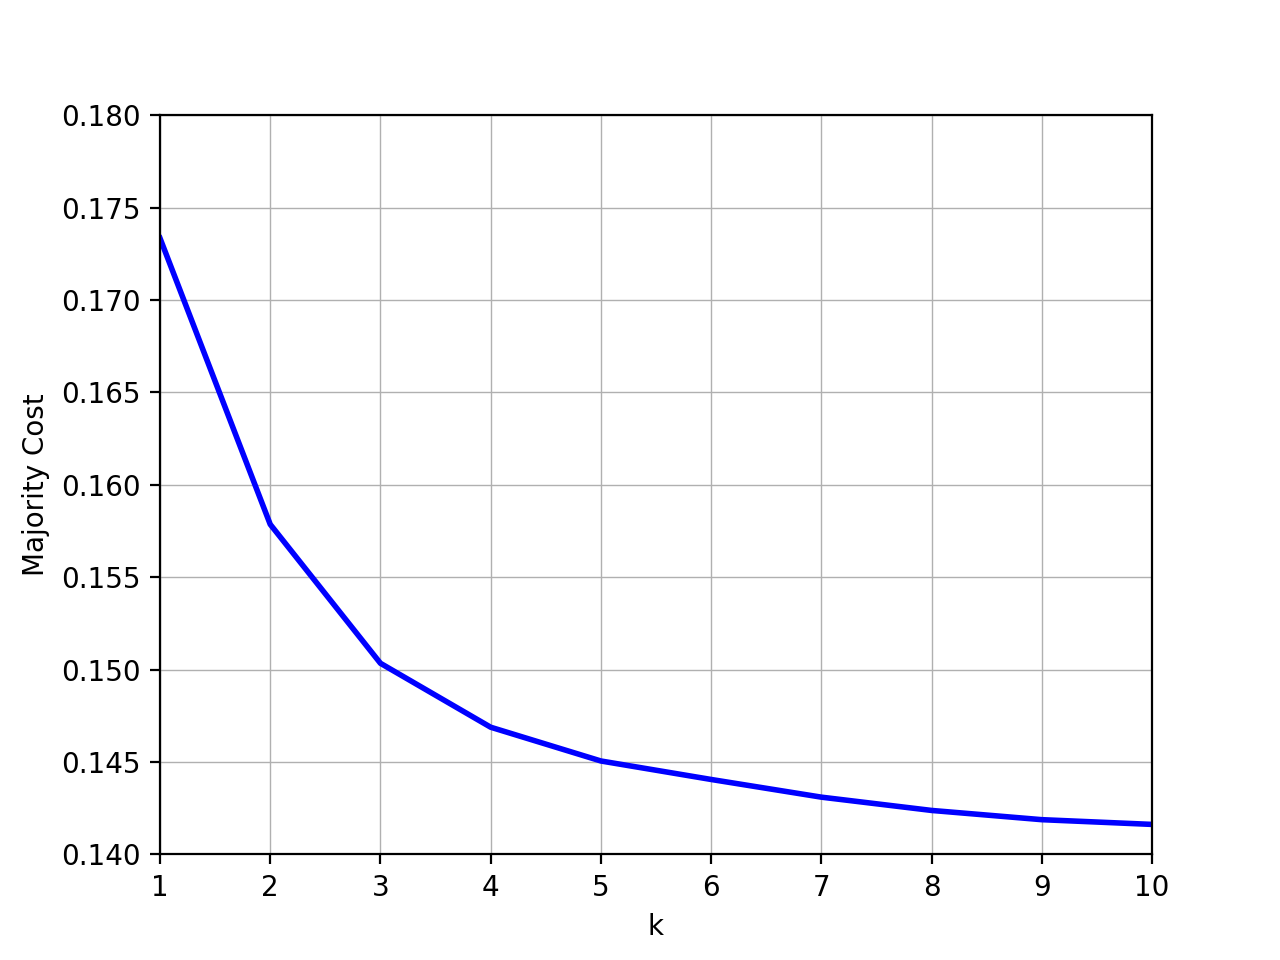
\includegraphics[width=\linewidth]{plots/nell_sc_1000_top10}
\end{minipage}
\begin{minipage}{.45\textwidth}
  \centering
  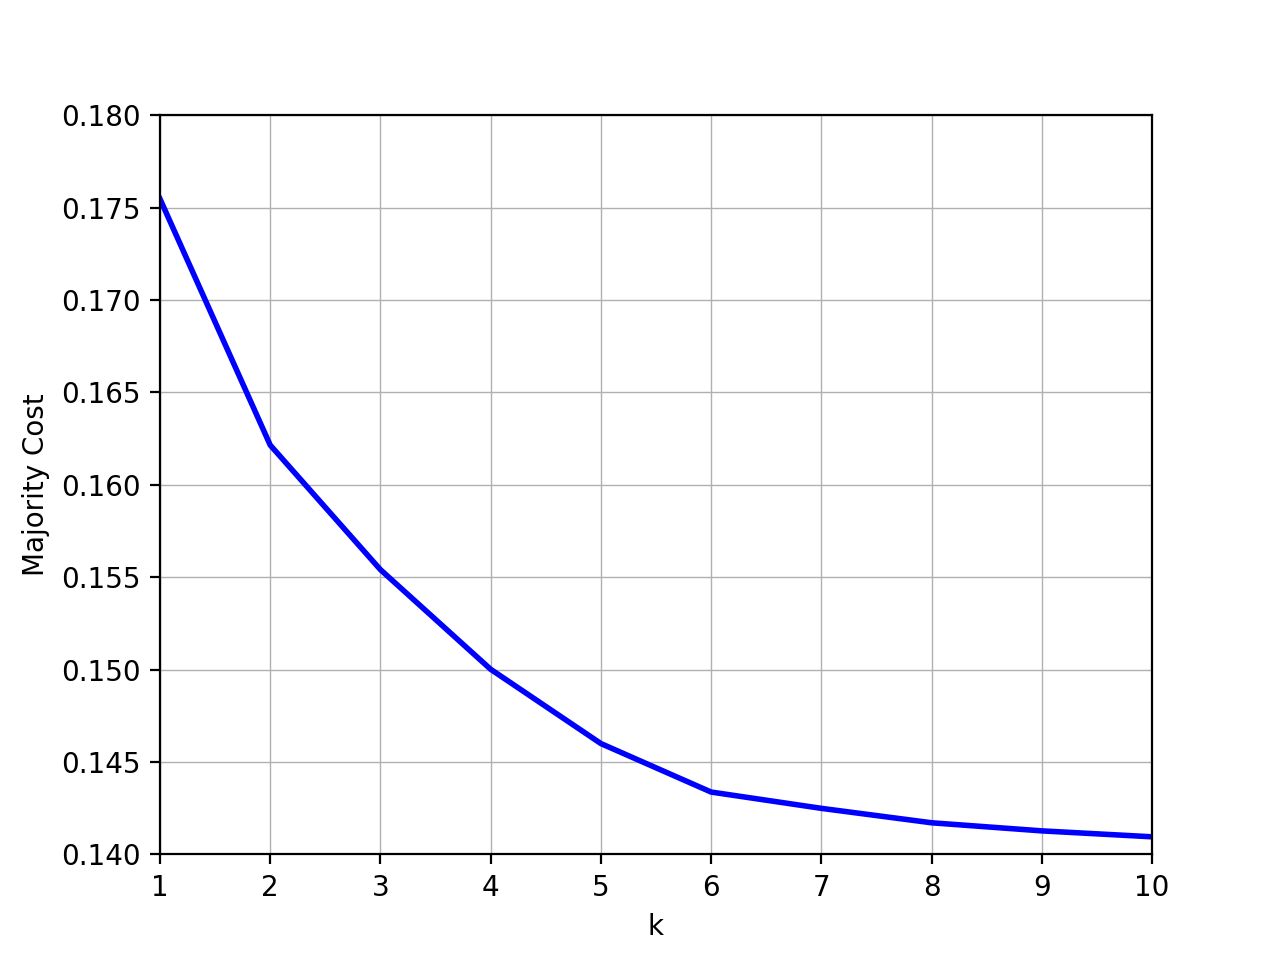
\includegraphics[width=\linewidth]{plots/nell_ac_1000_top10}
\end{minipage}
\caption{$\alpha$-linkage using 1000 points for each clustering instance gives minor improvements for the NELL data when clustering between single and complete (left) and average and complete linkage (right).}
\label{fig:nell1000top10}
\end{figure}

Also, we evaluated the corresponding clusters. As $\alpha$-linkage uses agglomerative hierarchical clustering, we can extract clusters at different levels starting with each noun phrase as its own cluster. Tables \ref{tbl:rooms}, \ref{tbl:clothing} and \ref{tbl:kitchenitems} show some examples for discovered categories.

\begin{table}[H]
  \makebox[\textwidth][c]{
  \small
  \begin{tabular}{cccc}
    \hline\hline
    \textbf{Luxury Room} & \textbf{Bathroom} & \textbf{Guest Room} & \textbf{Suite} \\ \hline
    spacious living room & large ensuite bathroom & elegant rooms & luxurious suites\\
    comfortable living room & spacious marble bathroom & three guest rooms & one bedroom suites\\
    guest room & one bathroom & large guest rooms & spacious suites\\
    lounge room & full bathroom & deluxe guest rooms & deluxe suites\\
    living room & upstairs bathroom & guests rooms & guest suites\\
    superior room & large bathroom & spacious air conditioned rooms & bedroom suites\\
    sleeping room & ensuite bathroom & furnished guest rooms & whirlpool suites\\
    main bedroom & elegant bathroom & comfortable guest rooms & three suites\\
    \hline
  \end{tabular}
  }
  \caption{Proposed Subcategories for ``Office Building Room''.}
  \label{tbl:rooms}
\end{table}

\begin{table}[H]
  \makebox[\textwidth][c]{
  \small
  \begin{tabular}{ccccc}
    \hline\hline
    \textbf{Shoes} & \textbf{Uniform/Costume} & \textbf{Pants} & \textbf{Casual} & \textbf{Specialized} \\ \hline
    shoes & costume & kneepants & stocking cap & long stockings\\
    high heel shoes & work uniforms & baggy pants & workout clothes & wide brimmed hat\\
    sensible shoes & outfits & loose fitting pants & casual clothes & casual wear\\
    old shoes & period costume & slacks & baseball caps & black stockings\\
    pointe shoes & folk costumes & black shorts & skull caps & wear socks\\
    dark shoes & halter top & special clothing & ball caps & high heels\\
    spira shoes & period costumes & white shorts & evening clothes & surf wear\\
    mens shoes & costumes & underpants & ball cap & wear gloves\\
    \hline
  \end{tabular}
  }
  \caption{Proposed Subcategories for ``Clothing''.}
  \label{tbl:clothing}
\end{table}

\begin{table}[H]
  \makebox[\textwidth][c]{
  \small
  \begin{tabular}{cccc}
    \hline\hline
    \textbf{Stove/Oven} & \textbf{Machines} & \textbf{Bowls} & \textbf{Baking Sheets} \\ \hline
    full size stove & cookie cutters & large mixing bowl & oiled baking sheet\\
    full size cooker & automatic washing machine & large serving bowl & rimmed baking sheet\\
    red hot stove & washing machine & small bowl & large baking sheet\\
    plastic jug & bread machine & single bowl & small baking sheet\\
    toaster & cookie cutter & separate bowl & prepared baking sheet\\
    greased baking dish & coffee machine & shallow bowl & ungreased baking sheet\\
    wood burning pizza oven & cooking spray & separate mixing bowl & hot plate\\
    ceramic top stove & coffee grinder & large bowl & greased baking sheet\\
    \hline
  \end{tabular}
  }
  \caption{Proposed Subcategories for ``Kitchen Item''.}
  \label{tbl:kitchenitems}
\end{table}

In addition to using the original features, we also use the word embeddings and the bag-of-contexts representations to evaluate these experiments.

\todo[inline]{Add experiments for new features.}

\paragraph{MNIST Experiments.} For the MNIST images, we evaluate both describes experimental settings with combinations of five out of the ten target classes. In addition to using the raw pixel features. To cluster the data, we set up $10 \choose 5$ $= 252$ different experiments by selecting all combinations of five out of the ten labels. In order to do so in efficient time, we subsample the dataset to 200 points for each label, so one experiment will cluster 1000 points. First, we evaluated the results for both average to complete and single to complete linkage for several batches. Note that we do not discuss the interpolation between single to average linkage in this and the following paragraphs, as experiments did not lead to improvements. First, we show the experiments for the six first batches $b_i, i \in \{0, 1, 2, 3, 4, 5\}$ for interpolating between single and complete linkage.

\begin{figure}[h]
\centering
\begin{minipage}{.3\textwidth}
  \centering
  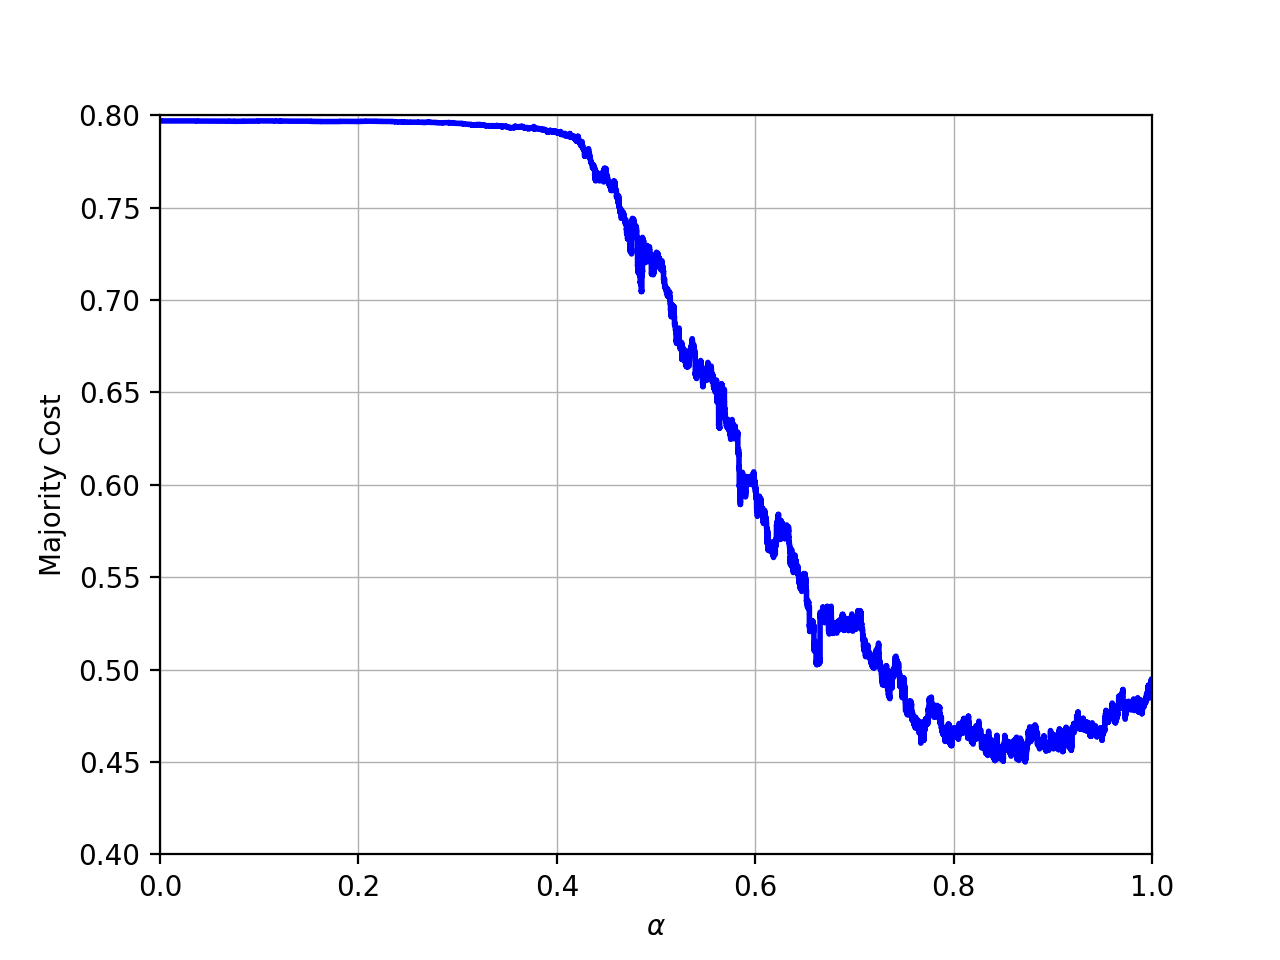
\includegraphics[width=\linewidth]{plots/mnist-sc-0}
\end{minipage}
\begin{minipage}{.3\textwidth}
  \centering
  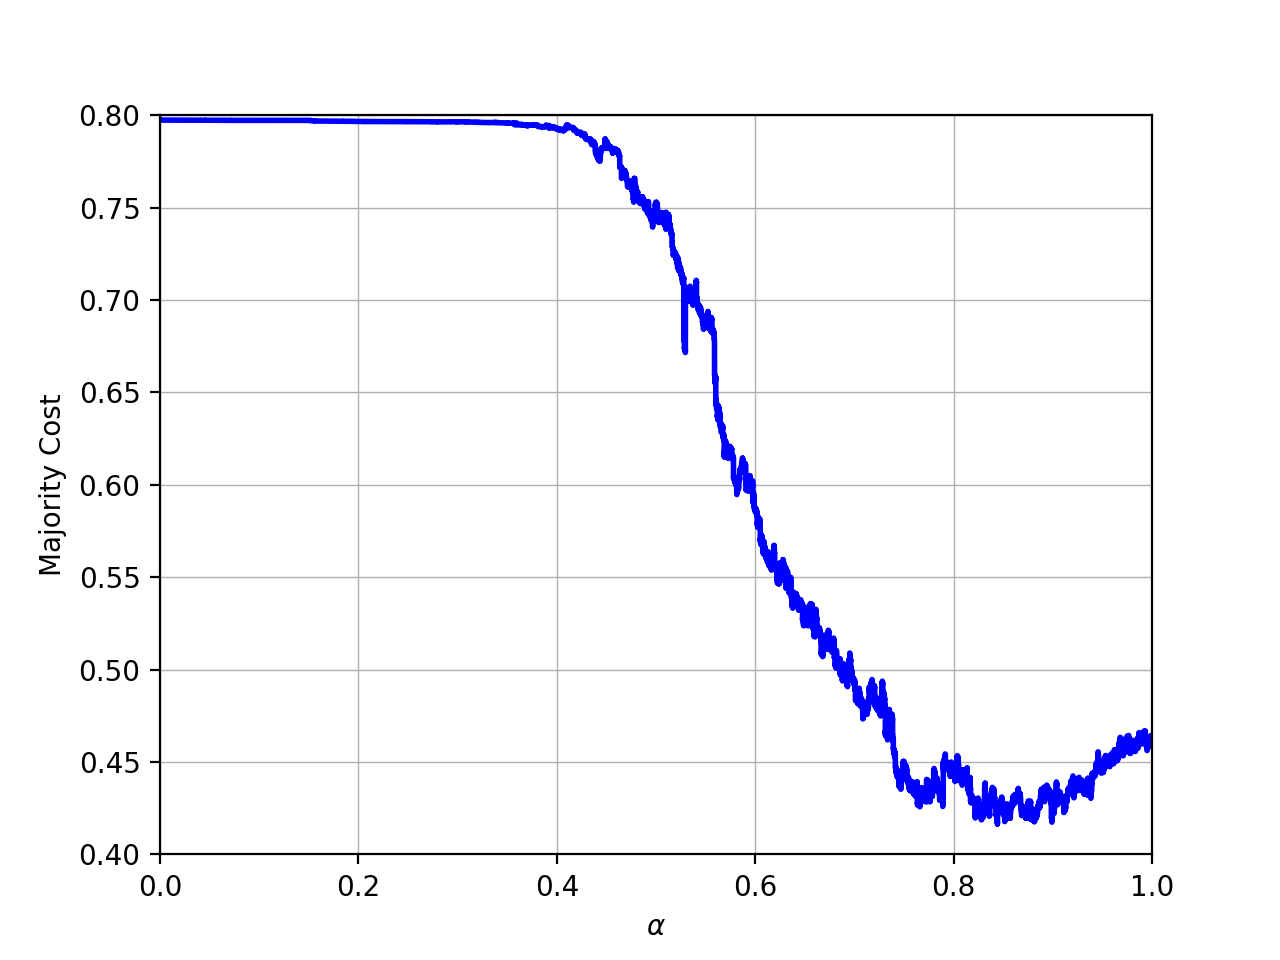
\includegraphics[width=\linewidth]{plots/mnist-sc-1}
\end{minipage}
\begin{minipage}{.3\textwidth}
  \centering
  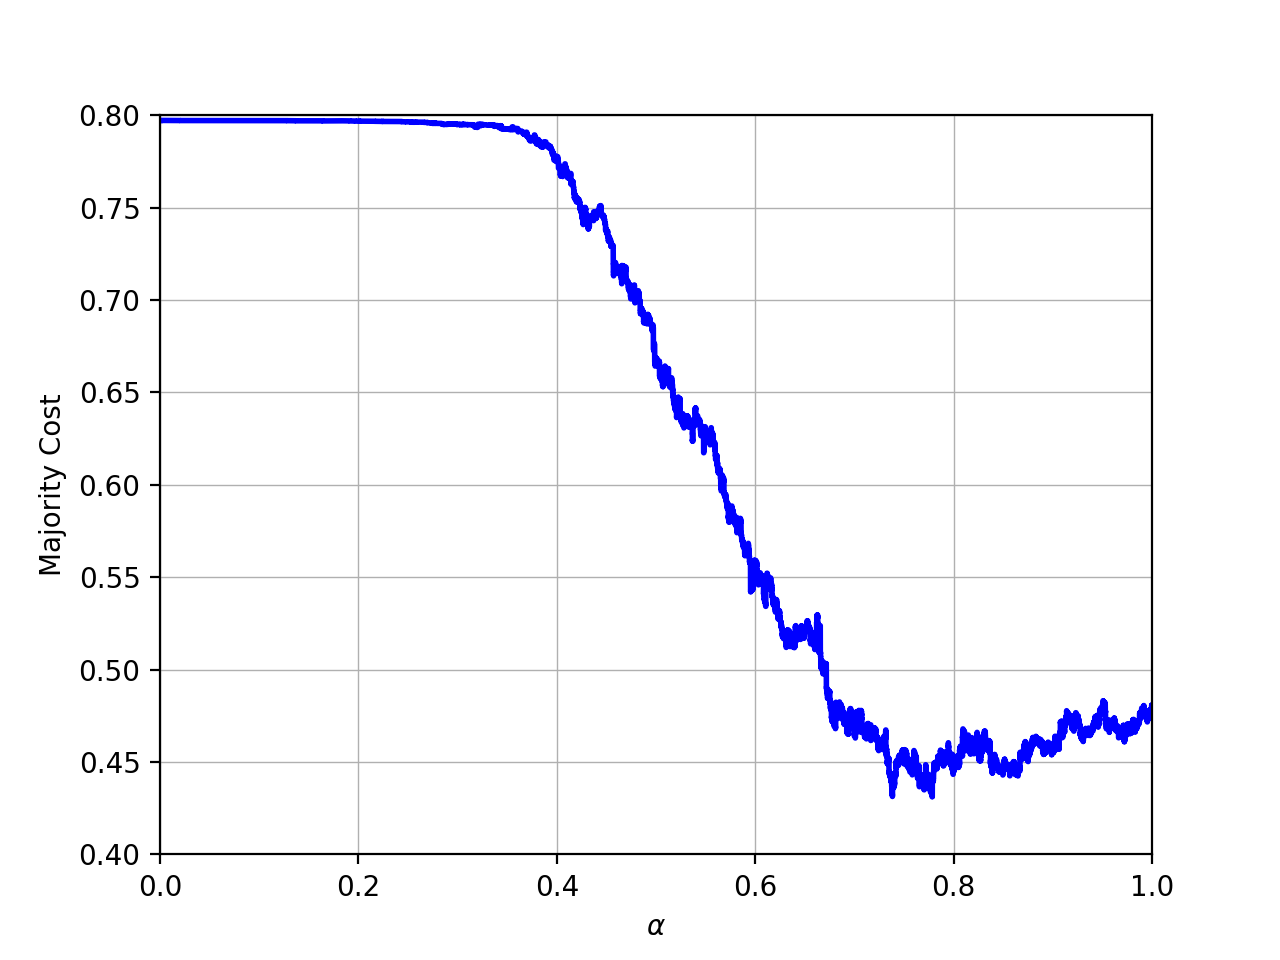
\includegraphics[width=\linewidth]{plots/mnist-sc-2}
\end{minipage}
\begin{minipage}{.3\textwidth}
  \centering
  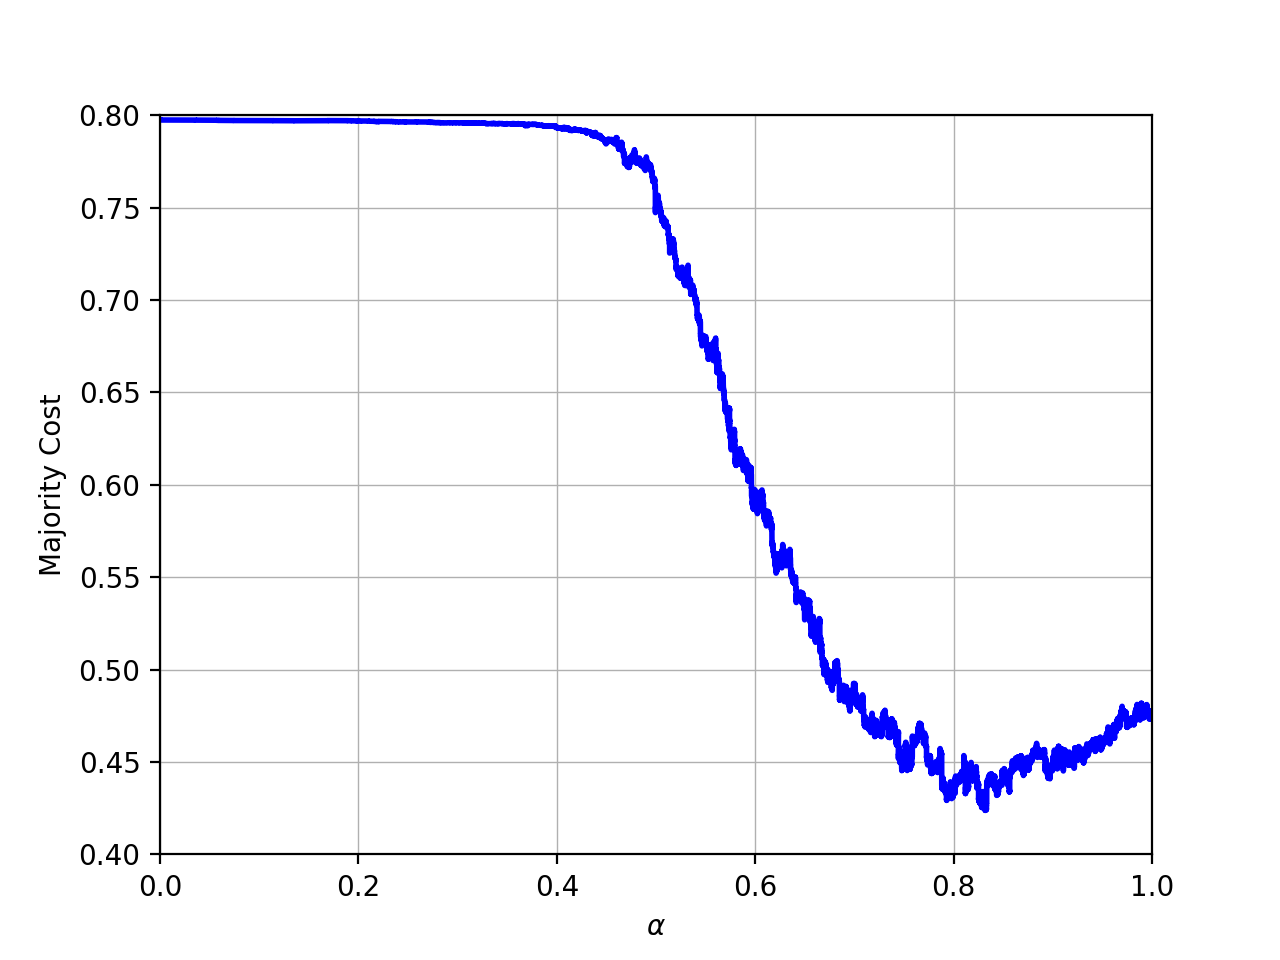
\includegraphics[width=\linewidth]{plots/mnist-sc-3}
\end{minipage}
\begin{minipage}{.3\textwidth}
  \centering
  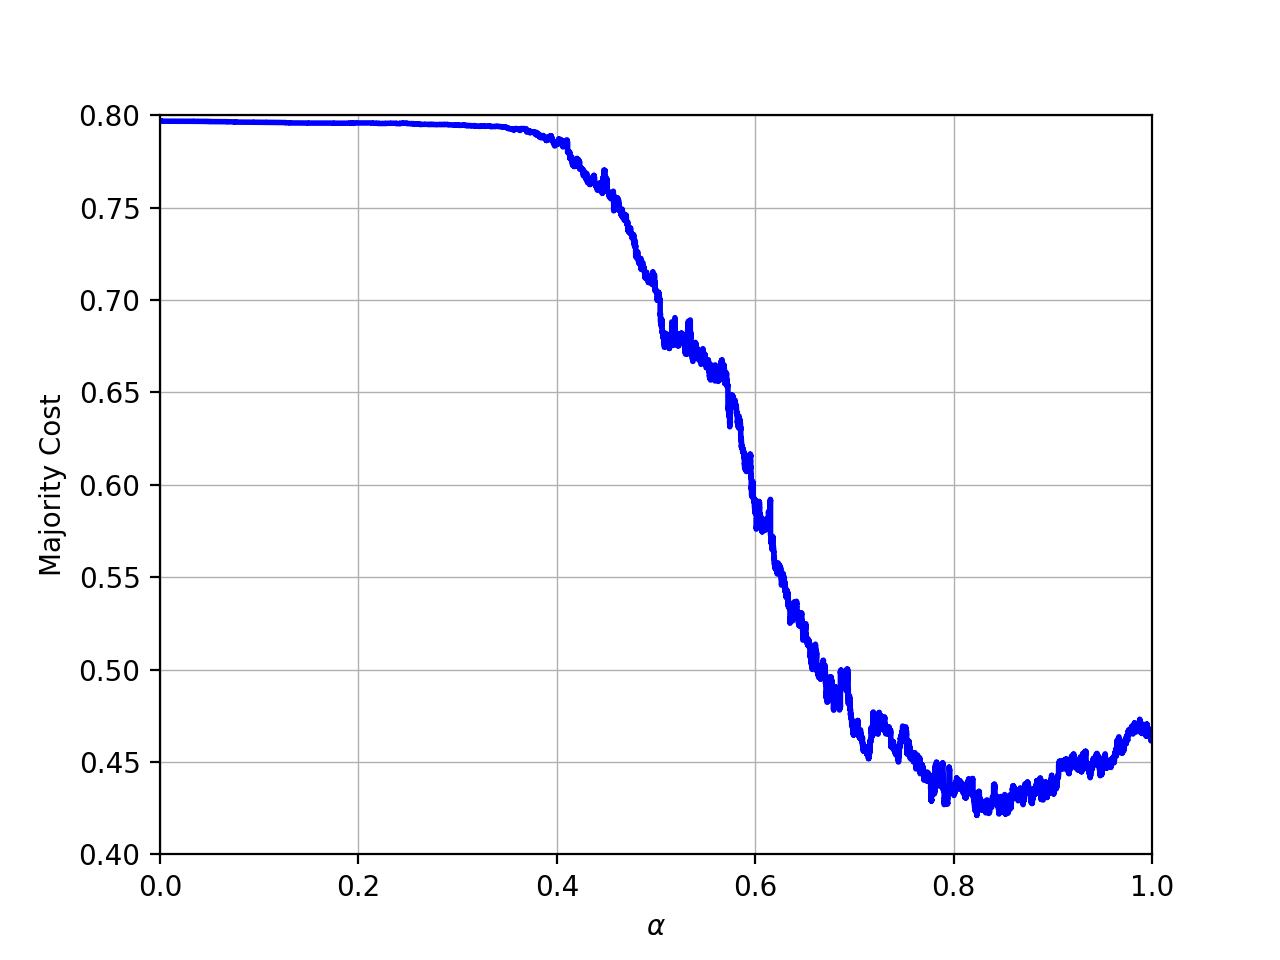
\includegraphics[width=\linewidth]{plots/mnist-sc-4}
\end{minipage}
\begin{minipage}{.3\textwidth}
  \centering
  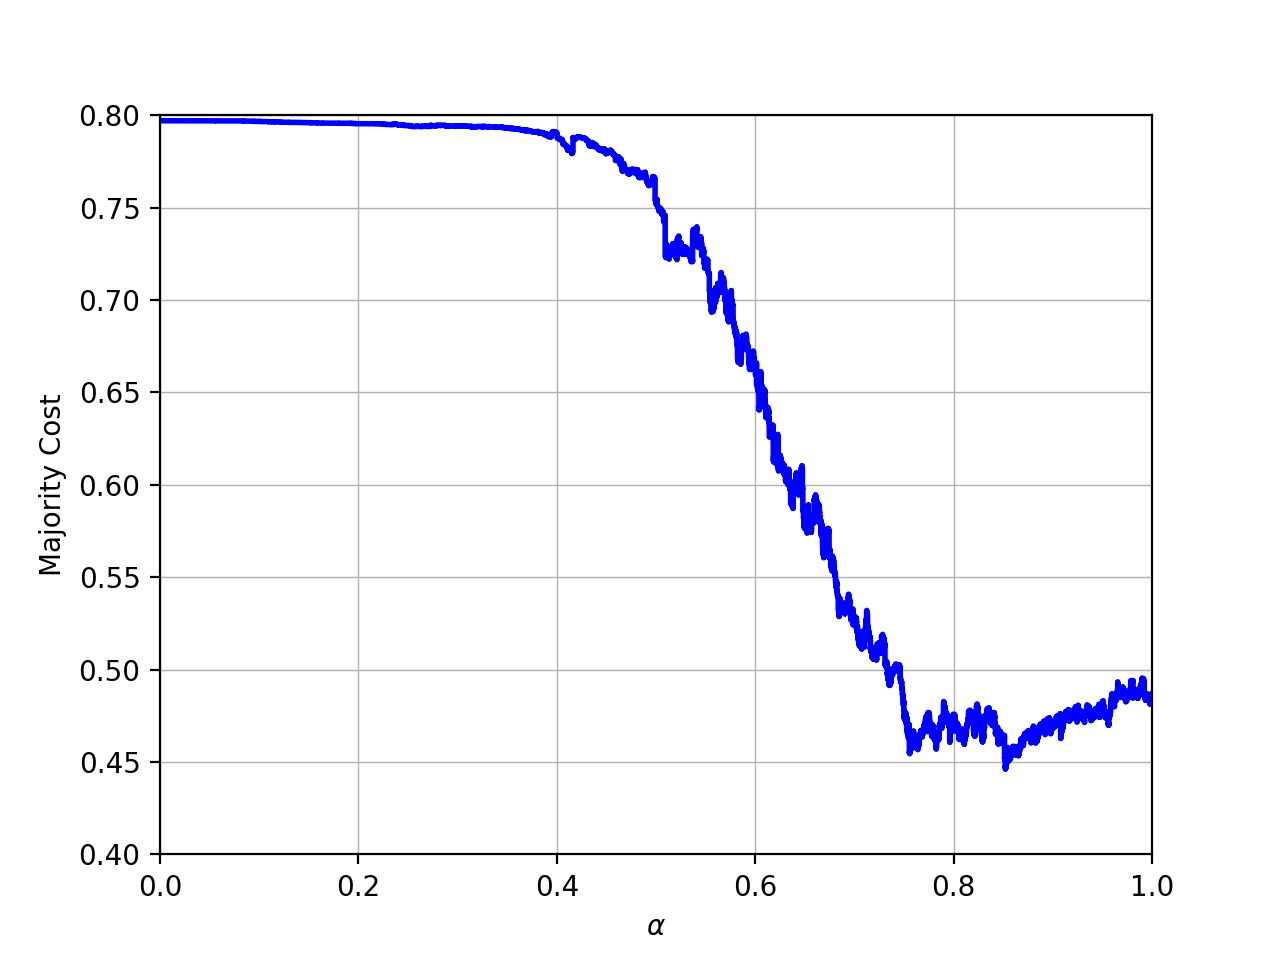
\includegraphics[width=\linewidth]{plots/mnist-sc-5}
\end{minipage}
\caption{Over the first six batches of the MNIST data, interpolating between single and complete linkage shows a similar behavior.}
\label{fig:mnistscbatches}
\end{figure}

As shown in figure \ref{fig:mnistscbatches}, the clustering over the first six batches leads to very similar curves with slightly different errors. Table \ref{table:mnistscbatches} evaluates the results in more detail.

\begin{table}[H]
    \centering
    \begin{tabular}{|l | l l l l l l |}
    \hline
    Strategy & Batch 0 & Batch 1 & Batch 2 & Batch 3 & Batch 4 & Batch 5\\ \hline
    Single Linkage & 0.796901 & 0.797345 & 0.797171 & 0.797405 & 0.796766 & 0.797024\\
    Complete Linkage & 0.490468 & 0.461063 & 0.479825 & 0.475329 & 0.463321 & 0.487111\\
    $\alpha_{opt}$ & 0.87228 & 0.84419 & 0.778498 & 0.83199 & 0.82338 & 0.852251\\
    $cost_{opt}$ & 0.450012 & 0.416433 & 0.431143 & 0.423786 & 0.421103 & 0.446032\\
    $\Delta cost$ & 4.0456\% & 4.463\% & 4.8682\% & 5.1543\% & 4.2218\% & 4.1079\%\\\hline
    \end{tabular}
    \caption{$\alpha$-linkage reduces the cost of the MNIST dataset by up to $\Delta_{max} cost = 5.1543\%$ when interpolating between single and complete linkage.}
    \label{table:mnistscbatches}
\end{table}

Table \ref{table:mnistscbatches} leads to several observations. Clustering points of five classes with a random guess will result in an error of $80\%$. As for all batches single linkage results in an error between $79\%$ and $80\%$, we note that single linkage performs similar than a random guess would. Thus, single linkage is not suitable for the MNIST data. In comparison, complete linkage results in errors below $50\%$ on just using the pixel data. It is not necessarily a great result, but it indicates that grouping high-dimensional pixel features with unsupervised learning can work. Also, we note that the parameter $\alpha_{opt}$ doesn't vary that much and also we notice in figure \ref{fig:mnistscbatches} that for $\alpha \in [0.75,1.0)$ we outperform complete linkage in all cases. As the results are very similar for the used batches, we also average over the batches in figure \ref{fig:mnistscbatchesavg}.

\begin{figure}[H]
    \centering
    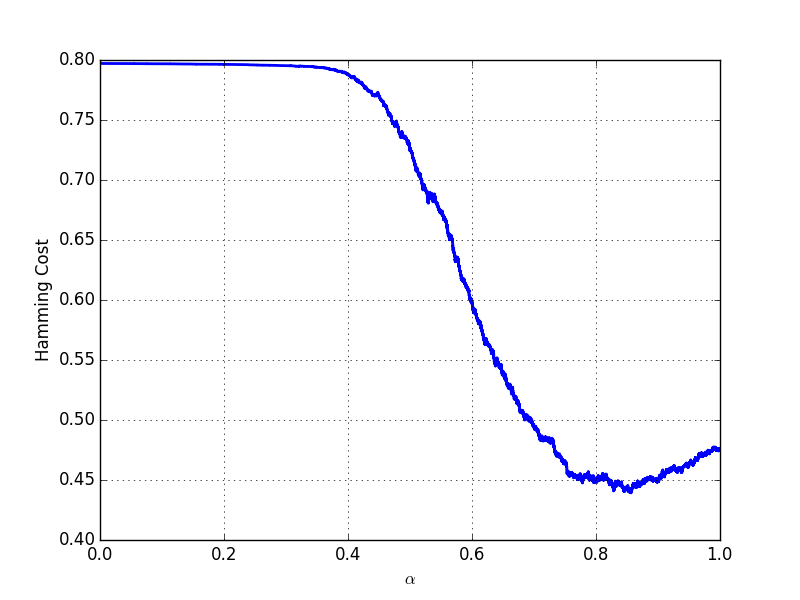
\includegraphics[width=0.5\textwidth]{plots/mnist-sc-averaged.png}
    \caption{Evaluating the first six batches of the MNIST data interpolating between single and complete linkage results in major improvements over both single and complete linkage.}
    \label{fig:mnistscbatchesavg}
\end{figure}

\begin{table}[H]
    \centering
    \begin{tabular}{|l | l |}
    \hline
    Strategy & Hamming Cost\\ \hline
    Single Linkage & 0.797102\\
    Complete Linkage & 0.476186\\
    $\alpha_{opt}$ & 0.857\\
    $cost_{opt}$ & 0.439207\\
    $\Delta cost$ & 3.6979\%\\\hline
    \end{tabular}
    \caption{Over the first 12,000 points of the MNIST dataset interpolating between single and complete linkage improves hamming cost by $3.7\%$ }
    \label{table:mnist1000avgsc}
\end{table}

Figure \ref{fig:mnistscbatchesavg} and table \ref{table:mnist1000avgsc} show that by applying $\alpha$-linkage interpolating between single and complete linkage we improve the hamming cost by $3.7\%$ over the first six data batches, i.e. the first 12,000 points of the dataset. Next, we evaluate the randomized experiments for the same interpolation method, where we average over 512 experiments that are run with random label subsets and randomly selected points for each of the selected labels. Figure \ref{fig:mnistscrandom} shows that in this setting we obtain a very similar curve as in the other setting (figure \ref{fig:mnistscbatchesavg}).

\begin{figure}[H]
    \centering
    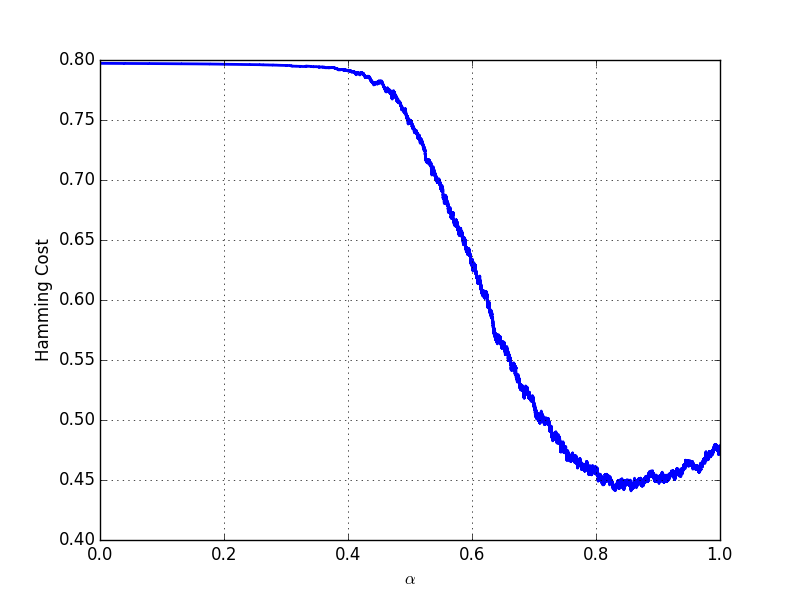
\includegraphics[width=0.5\textwidth]{plots/mnist-sc-random.png}
    \caption{Selecting labels and points randomly leads to a similar curve when interpolating between single and complete linkage using the MNIST data.}
    \label{fig:mnistscrandom}
\end{figure}

\begin{table}[H]
    \centering
    \begin{tabular}{|l | l | l |}
    \hline
    Strategy & Hamming Cost (Batch) & Hamming Cost (Random)\\ \hline
    Single Linkage & 0.797102 & 0.797215\\
    Complete Linkage & 0.476186 & 0.476355\\
    $\alpha_{opt}$ & 0.857 & 0.857\\
    $cost_{opt}$ & 0.439207 & 0.440932\\
    $\Delta cost$ & 3.6979\% & 3.5423\%\\\hline
    \end{tabular}
    \caption{Evaluating the randomized setting leads to exactly the same parameter $\alpha_{opt}$ and a similar cost improvement as in the batch setting for the MNIST data.}
    \label{table:mnist1000randomsc}
\end{table}

Table \ref{table:mnist1000randomsc} compares the results for both settings when interpolating between single and complete linkage. We obtain very similar results for single and complete linkage. Also, the optimal parameter $\alpha_{opt}$ is the same in both settings leading to similar improvements in the hamming cost. This means that $\alpha$-linkage is robust over the entire MNIST distribution and with an improvement of more than $3\%$ towards complete linkage it outperforms both used linkage strategies by a major difference. In addition, we also evaluate the greedy parameter advising for the previous experiments.\\

\begin{figure}[H]
\centering
\begin{minipage}{.45\textwidth}
  \centering
  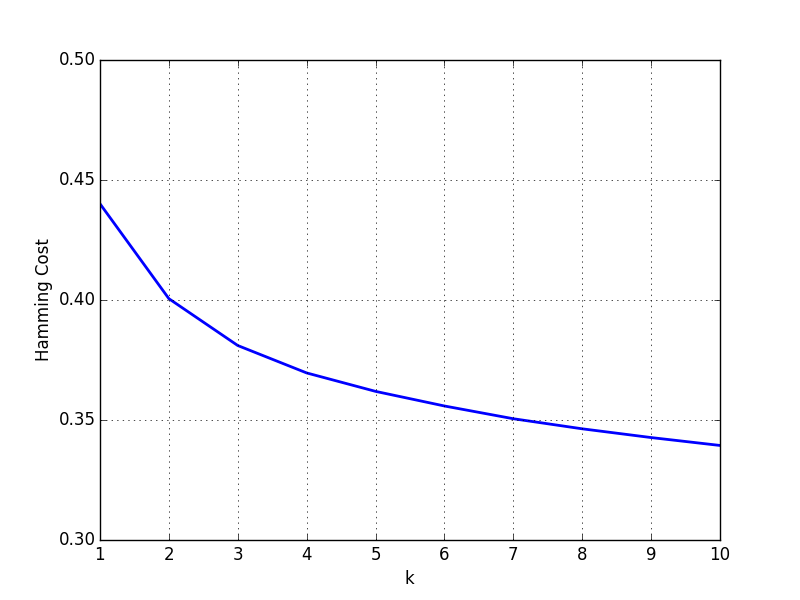
\includegraphics[width=\linewidth]{plots/mnist-sc-top-10}
\end{minipage}
\begin{minipage}{.45\textwidth}
  \centering
  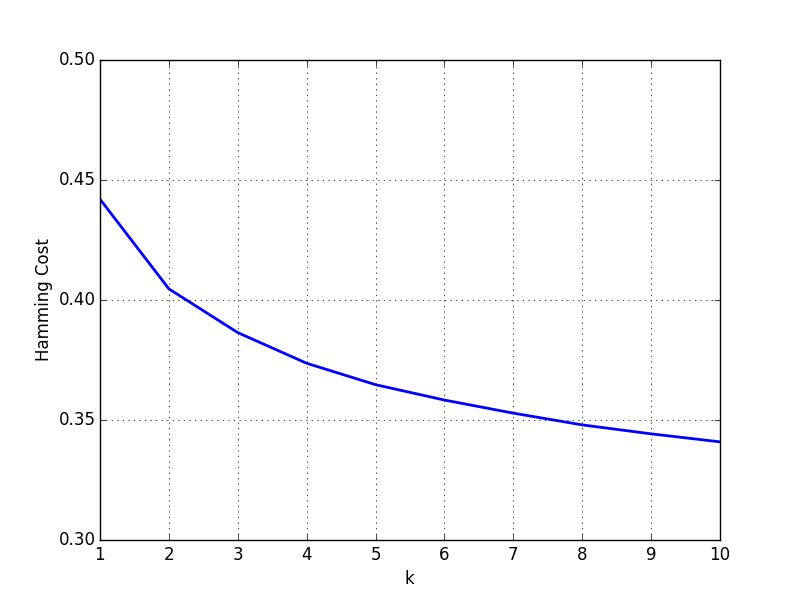
\includegraphics[width=\linewidth]{plots/mnist-sc-random-top-10}
\end{minipage}
\caption{}
\label{fig:mnistsctop10}
\end{figure}

Figure \ref{fig:mnistsctop10} shows that we again obtain very similar results for the batch setting (left) and the random setting (right). By using $k = 3$ parameters $\alpha^*$ the cost drops more than $5\%$ in addition to less than $38\%$. In comparison to the best linkage strategy, i.e. complete linkage, this is an improvement of $\approx 10\%$.\\

Similar to that, we also interpolate between average and complete linkage and evaluate both the batch and the random setting. Figure \ref{fig:mnist1000acbatch} and table \ref{table:mnist1000acbatch} show that the results of the different batches vary much. On the one hand, the parameters $\alpha_{opt}$ have a wider range ($\alpha_{opt} \in [0.53,0.81]$), but on the other hand, we get slightly larger improvements for the hamming cost in comparison to complete linkage.

\begin{figure}[H]
\centering
\begin{minipage}{.3\textwidth}
  \centering
  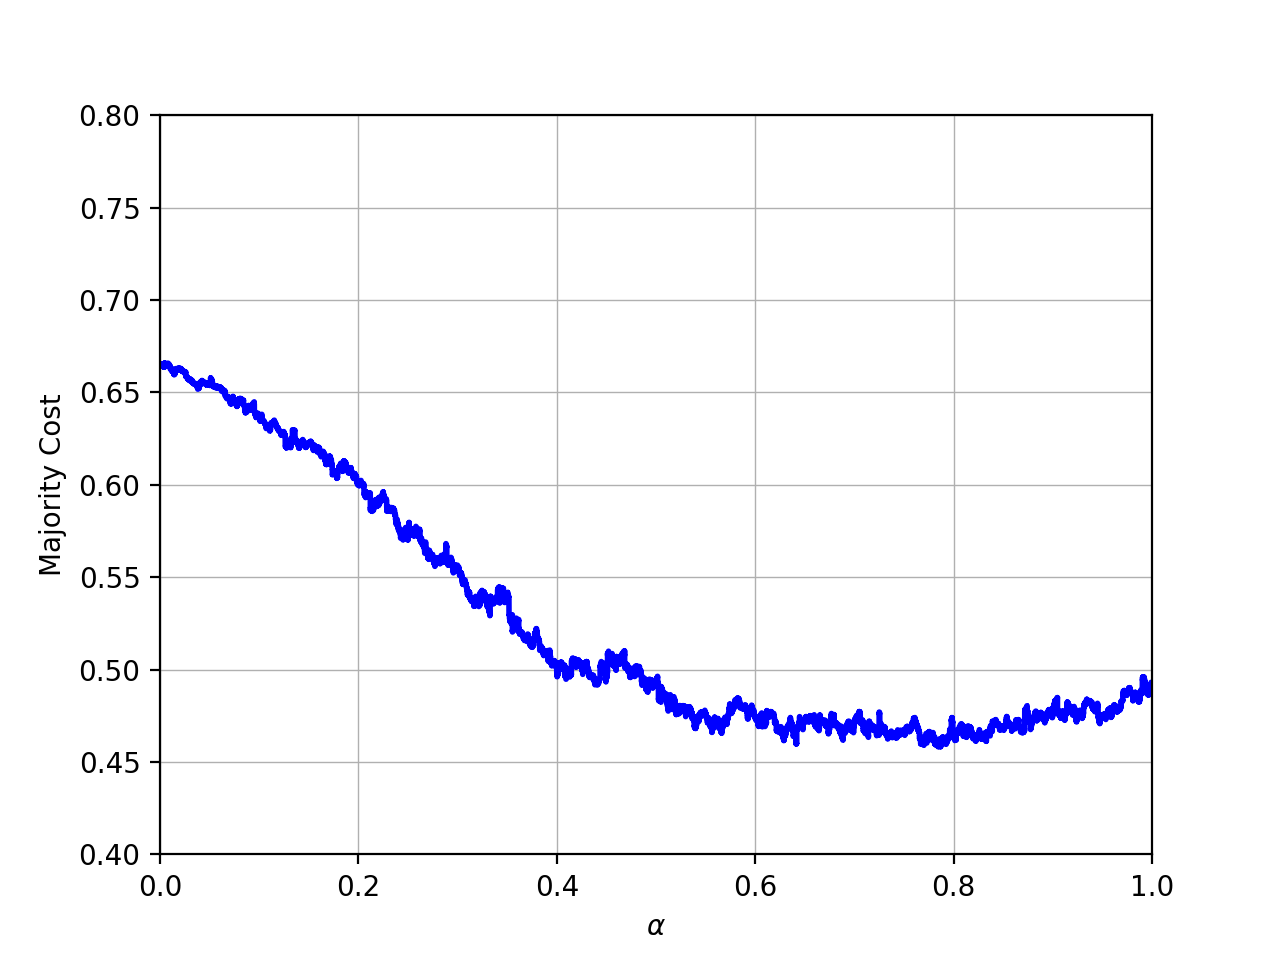
\includegraphics[width=\linewidth]{plots/mnist-ac-0}
\end{minipage}
\begin{minipage}{.3\textwidth}
  \centering
  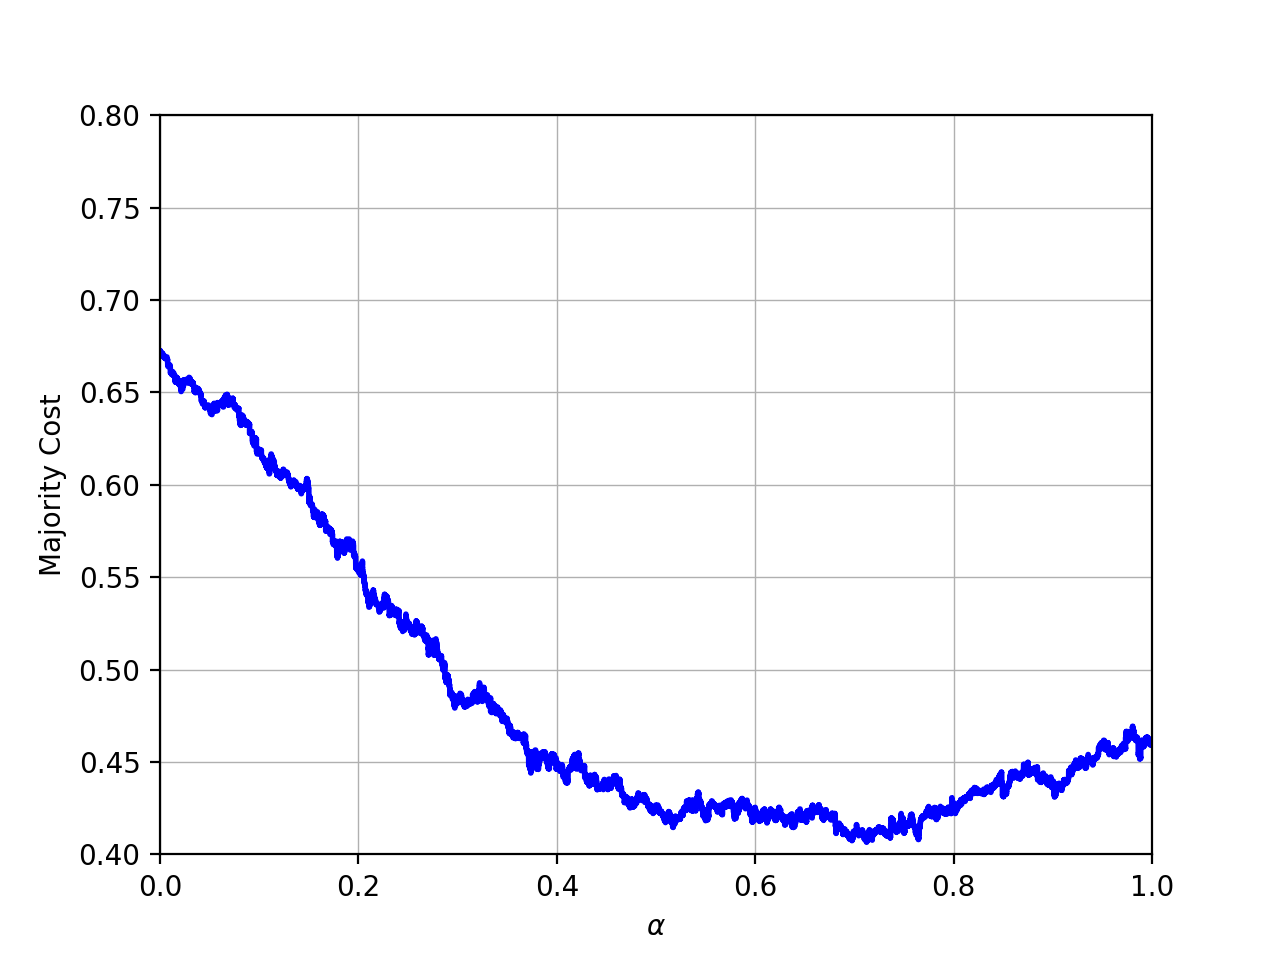
\includegraphics[width=\linewidth]{plots/mnist-ac-1}
\end{minipage}
\begin{minipage}{.3\textwidth}
  \centering
  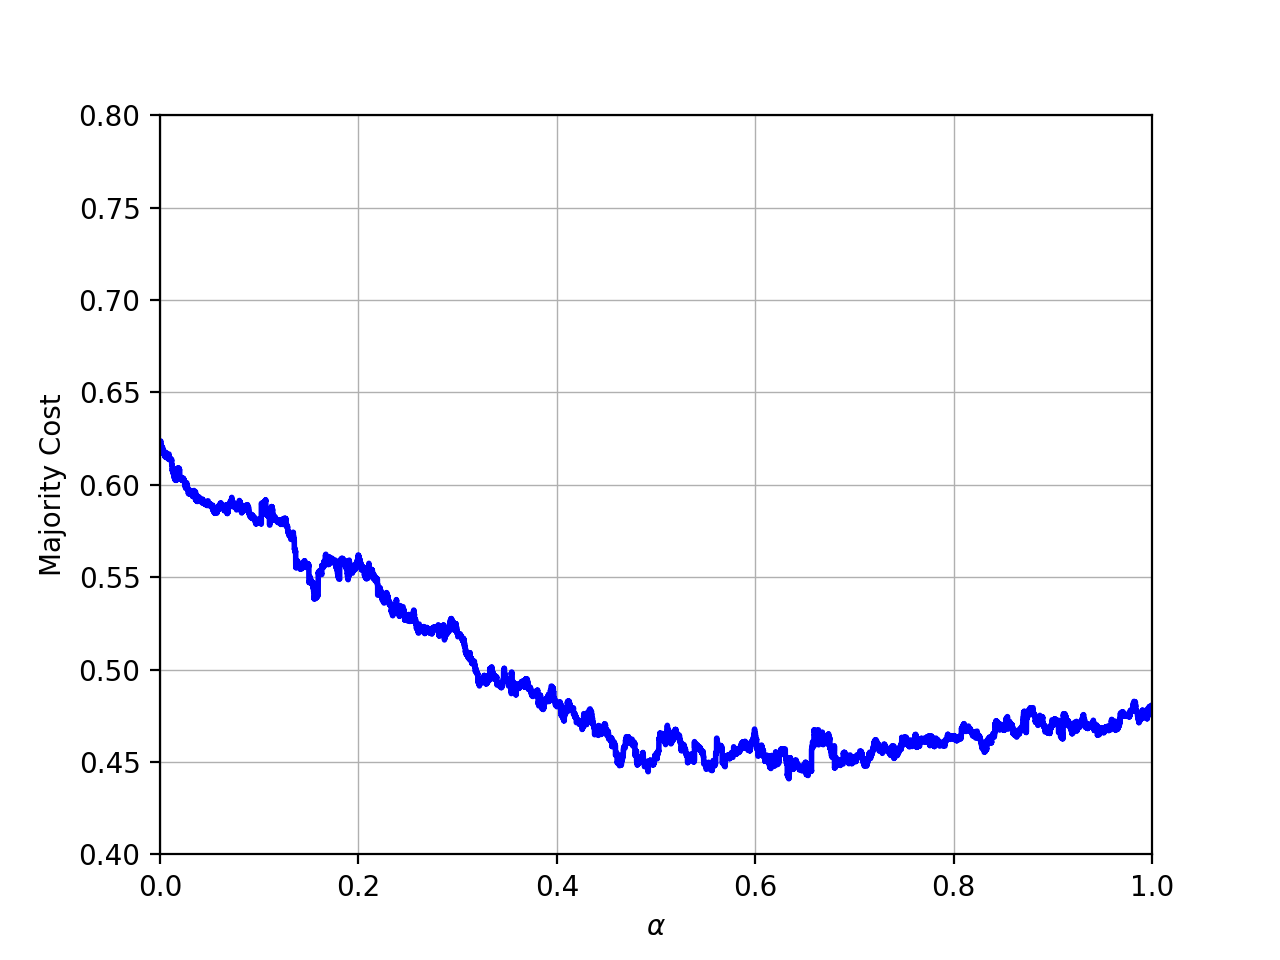
\includegraphics[width=\linewidth]{plots/mnist-ac-2}
\end{minipage}
\begin{minipage}{.3\textwidth}
  \centering
  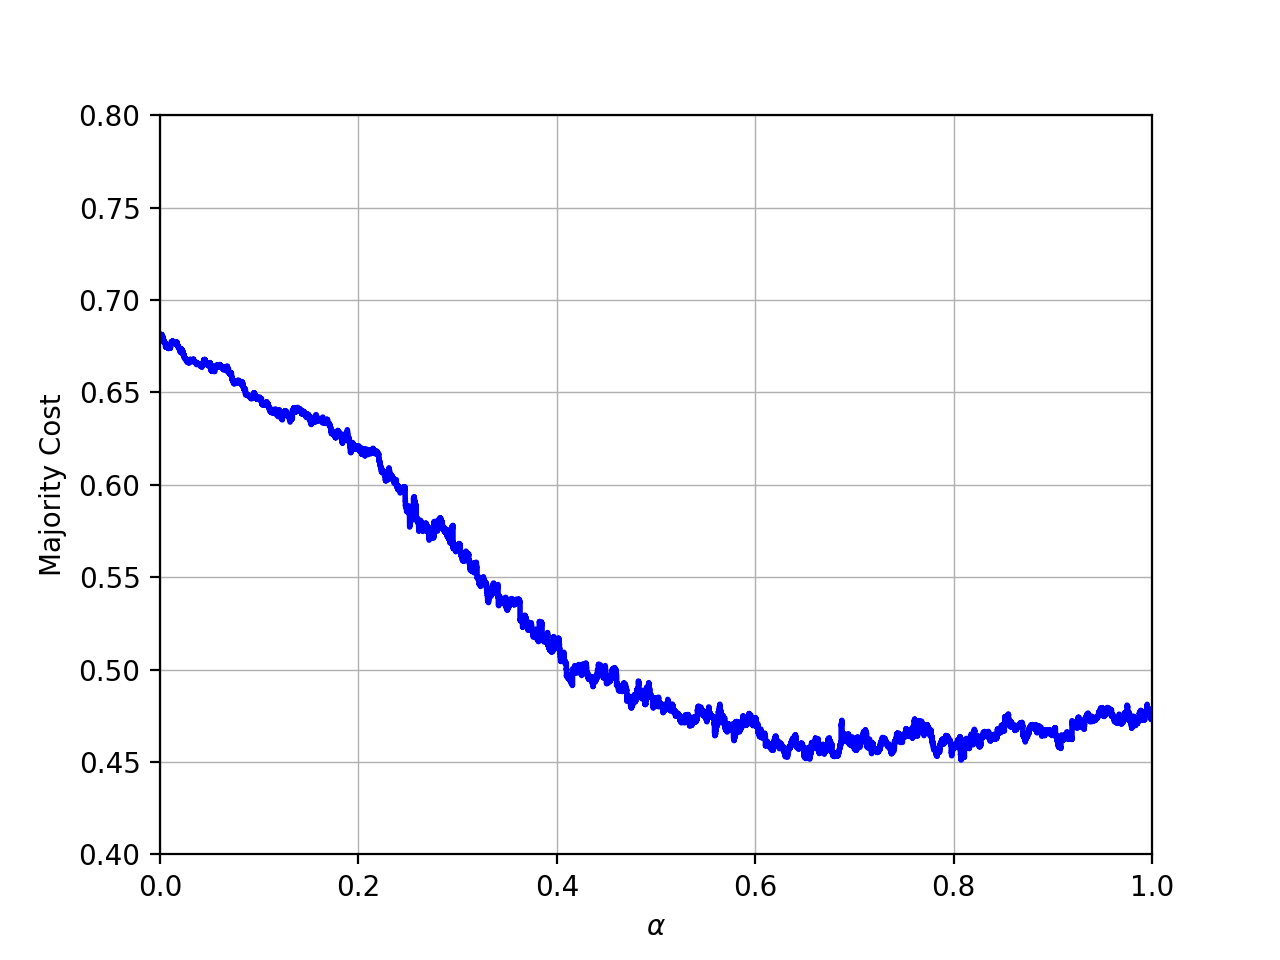
\includegraphics[width=\linewidth]{plots/mnist-ac-3}
\end{minipage}
\begin{minipage}{.3\textwidth}
  \centering
  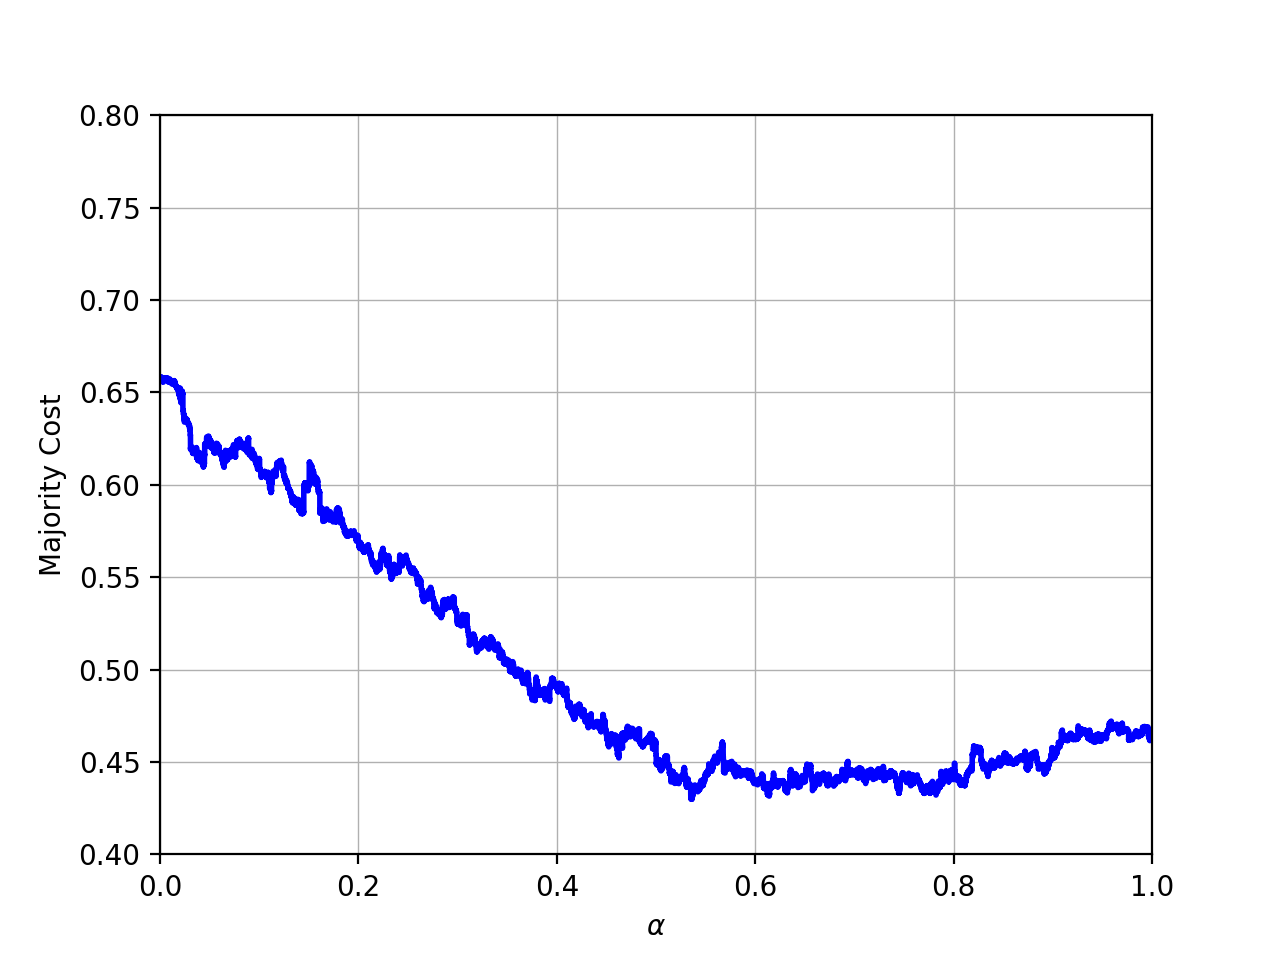
\includegraphics[width=\linewidth]{plots/mnist-ac-4}
\end{minipage}
\begin{minipage}{.3\textwidth}
  \centering
  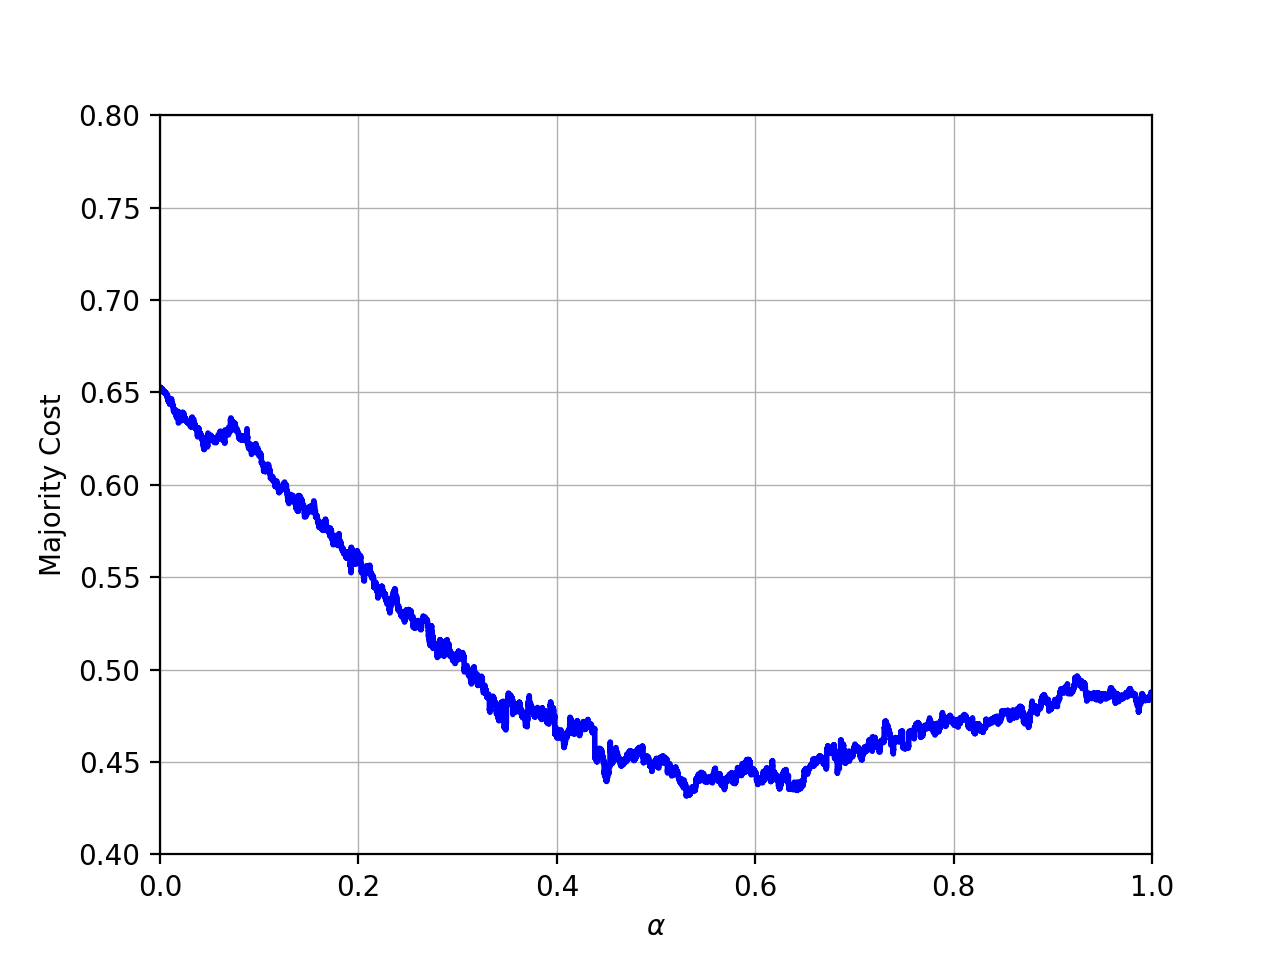
\includegraphics[width=\linewidth]{plots/mnist-ac-5}
\end{minipage}
\caption{Over the first six batches of the MNIST data, interpolating between average and complete linkage shows quite different curves.}
\label{fig:mnist1000acbatch}
\end{figure}

\begin{table}[h]
    \centering
    \begin{tabular}{|l | l l l l l l |}
    \hline
    Strategy & Batch 0 & Batch 1 & Batch 2 & Batch 3 & Batch 4 & Batch 5\\ \hline
    Average Linkage & 0.664952 & 0.672583 & 0.623325 & 0.679929 & 0.657857 & 0.652774\\
    Complete Linkage & 0.490468 & 0.461063 & 0.479825 & 0.475329 & 0.463321 & 0.487111\\
    $\alpha_{opt}$ & 0.7869 & 0.7124 & 0.634 & 0.807697 & 0.536073 & 0.5305\\
    $cost_{opt}$ & 0.458167 & 0.406563 & 0.440964 & 0.451063 & 0.429849 & 0.431631\\
    $\Delta cost$ & 3.2301\% & 5.45\% & 3.8861\% & 2.4266\% & 3.3472\% & 5.548\%\\\hline
    \end{tabular}
    \caption{$\alpha$-linkage reduces the cost of the MNIST dataset by up to $\Delta_{max} cost = 5.548\%$ when interpolating between average and complete linkage.}
    \label{table:mnist1000acbatch}
\end{table}

\begin{figure}[h]
\centering
\begin{minipage}{.45\textwidth}
  \centering
  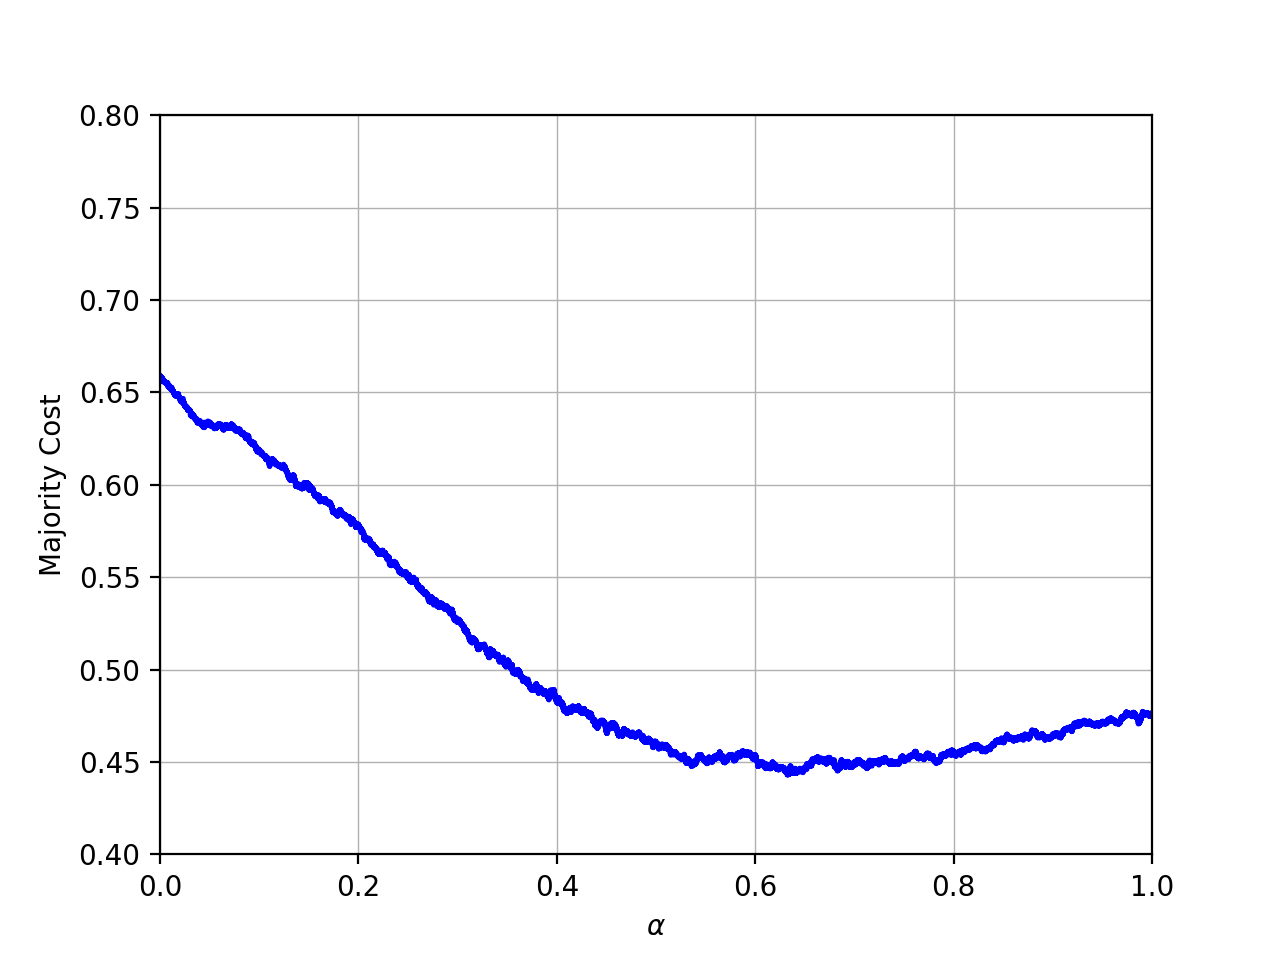
\includegraphics[width=\linewidth]{plots/mnist-ac-averaged}
\end{minipage}
\begin{minipage}{.45\textwidth}
  \centering
  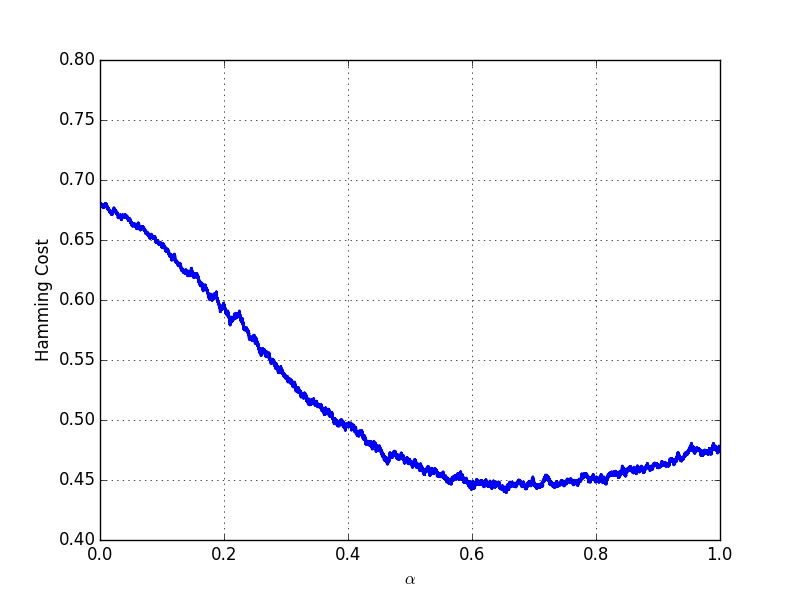
\includegraphics[width=\linewidth]{plots/mnist-ac-random}
\end{minipage}
\caption{Comparing the batch and the random experients for the MNIST data when interpolating between average and complete linkage leads to similar curves.}
\label{fig:mnistacavg}
\end{figure}

Figure \ref{fig:mnistacavg} shows the comparison between the batch (left) and the random experiments (right). In general, we obtain similarly looking curves, but elaborate the results further in table \ref{table:mnistacavg}.

\begin{table}[h]
    \centering
    \begin{tabular}{|l | l | l |}
    \hline
    Strategy & Hamming Cost (Batch) & Hamming Cost (Random)\\ \hline
    Average Linkage & 0.65857 & 0.679936\\
    Complete Linkage & 0.476187 & 0.476328\\
    $\alpha_{opt}$ & 0.633 & 0.656\\
    $cost_{opt}$ & 0.44314 & 0.439632\\
    $\Delta cost$ & 3.3047\% & 3.6696\%\\\hline
    \end{tabular}
    \caption{}
    \label{table:mnistacavg}
\end{table}

\begin{figure}[H]
\centering
\begin{minipage}{.45\textwidth}
  \centering
  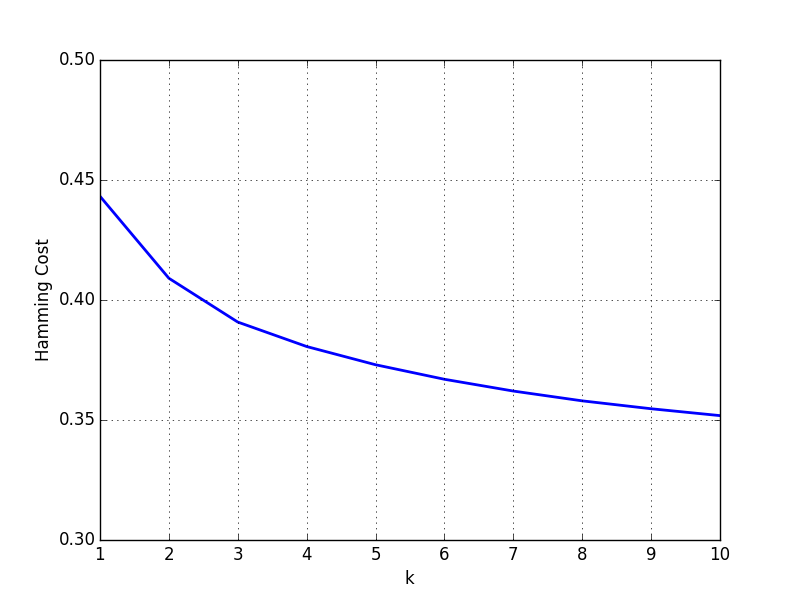
\includegraphics[width=\linewidth]{plots/mnist-ac-top-10}
\end{minipage}
\begin{minipage}{.45\textwidth}
  \centering
  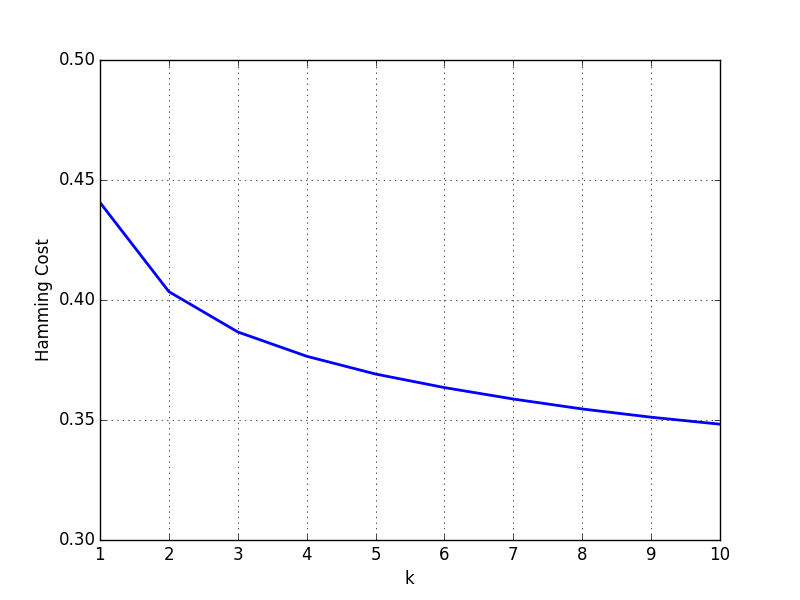
\includegraphics[width=\linewidth]{plots/mnist-ac-random-top-10}
\end{minipage}
\caption{}
\label{fig:mnistactop10}
\end{figure}

Summarizing, we also obtained very positive results for $d_{AC}$, however the results were not as stable as for $d_{SC}$. In our experiments, we notice that $d_{SC}$ results in more discontinuities (factor $\approx 3$) than $d_{AC}$. This may be because the distance $d(\alpha)$ is wider spread for $d_{SC}$, i.e. $|d_{SC}(\alpha = 1) - d_{SC}(\alpha = 0)| > |d_{AC}(\alpha = 1) - d_{AC}(\alpha = 0)|$. However $d_{AC}$ is dependant on more points, so it may be an indicator for this observation, but not a proof. Figure \ref{fig:mnistactop10} also shows that parameter advising is using with a small value $k$ already and reduces the costs for $k = 3$ by $\approx 5\%$ in addition.

\paragraph{Learning MNIST features.} Differently to just using the raw pixel features, we here apply preprocessing techniques with the intention to generate more accurate clusterings. As in section \ref{sec:imagefeatures} described, we use a Convolutional Neural Network to learn a more robust and lower-dimensional feature representation. Therefore, we use the in appendix \ref{sec:cnnarchitecture} described architecture, train the network with all data and then extract the features by cutting off the last three layers of the network. This then results in a learned 128-dimensional representation for each image.

\begin{figure}[h]
\centering
\begin{minipage}{.45\textwidth}
  \centering
  \subcaptionbox{By evaluating all 252 combinations of five different labels, the average error goes down to $2.6\%$ that makes an improvement of $7.4\%$ compared to complete linkage.}
  {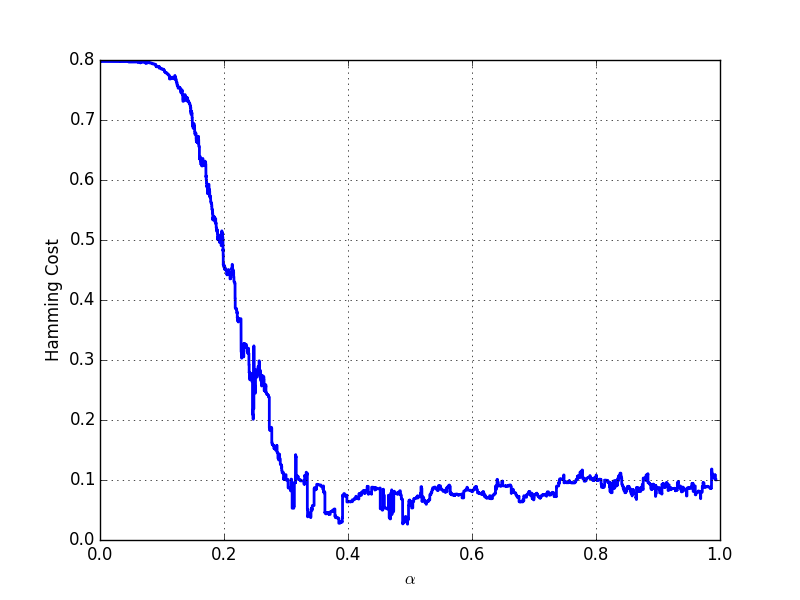
\includegraphics[width=\linewidth]{plots/mnist-cnn-avg}}
\end{minipage}\quad
\begin{minipage}{.45\textwidth}
  \centering
  \subcaptionbox{Evaluating 512 random sets of labels and points gives an eror of $7.1\%$ that is an improvement of $1.9\%$ compared to complete linkage.}
  {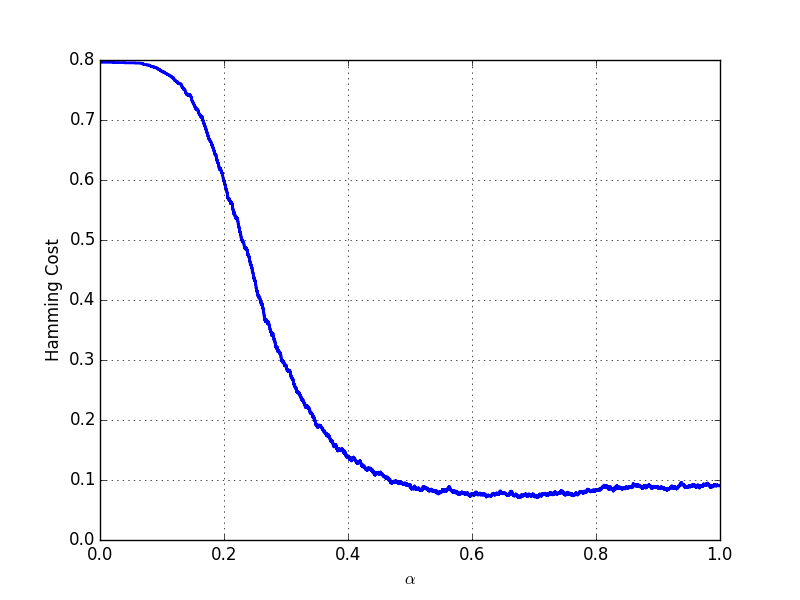
\includegraphics[width=\linewidth]{plots/mnist-cnn-random}}
\end{minipage}
\begin{minipage}{.45\textwidth}
  \centering
  \subcaptionbox{Considerung more than one optimal value to evaluate the experiments results in lower costs, e.g. using two values $\alpha_{opt}$ cuts the cost by $50\%$ and using three values results in a cost below $1\%$.}
  {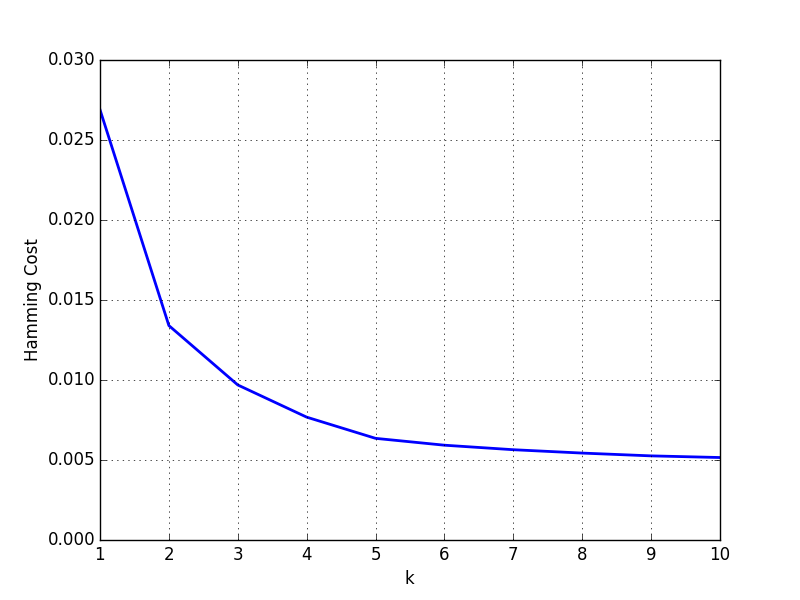
\includegraphics[width=\linewidth]{plots/mnist-cnn-sc-top-10}}
\end{minipage}\quad
\begin{minipage}{.45\textwidth}
  \centering
  \subcaptionbox{On random sets of labels and randomly selected points, taking more than one optimal value $\alpha_{opt}$ also gives major improvements. With three values the cost goes down below $3\%$ that is less than a half of the original optimum.}
  {\includegraphics[width=\linewidth]{plots/mnist-cnn-sc-random-top-10}}
\end{minipage}
\caption{By learning feature representations with a Convolutional Neural Network, we can reduce the overall error a lot compared to clustering raw pixel images.}
\label{fig:mnist1000cnn}
\end{figure}

Figure \ref{fig:mnist1000cnn} shows that single linkage still performs poorly, however the error for both complete linkage and the interval in between are much lower. Also, we note that the improvement using $\alpha$-linkage is large over both settings. However, a Convolutional Neural Network aims at recognizing the characters, so training on all images might be the sole cause of our improvements. Thus, it is more relevant for our experiments to either train the network on a subset of the data or to train the network on a different task in order to transfer the knowledge to unseen data or to a different task.

\paragraph{Learning Subsets of the MNIST Data.} As our goal is also to cluster unseen data, we evaluated another setup, where a CNN was trained on a subset of the dataset. In a first attempt, we trained it on the labels $\{0,1,2,3,4\}$ that are represented with 30,000 of the 60,000 points in the dataset. Figure \ref{fig:mnist1000cnnsub} shows that clustering unseen points (i.e. the CNN did not use these points for training) still results in a lower error than using the raw pixel features where combining seen and unseen points leads to results that are comparable to clusterings with features extracted from a neural network that was trained with all digits. In average, complete linkage resulted in an error of $22.1\%$. The cost for $\alpha_{opt} = 0.67$ is $20.7\%$ and makes an improvement of $1.4\%$. Interesting especially in this setting are the different results of seen and unseen data. In machine learning, the task of applying knowledge to unseen data is commonly known as zero-shot learning. While the error was $0.2\%$ for large parts of the seen data (i.e. clustering the digits $\{0,1,2,3,4\}$), the optimal cost for the unseen data (i.e. clustering the digits $\{5,6,7,8,9\}$) was $24.7\%$ for $\alpha_{opt} = 0.76$. \todo[inline]{plot and discuss randomized experiments}

\begin{figure}[H]
\centering
\begin{minipage}{.3\textwidth}
  \centering
  \subcaptionbox{The learned characters (i.e. labels $\{0,1,2,3,4\}$) can be clustered very well. Similar to training on all labels, the error goes down close to $0\%$.}
  {\includegraphics[width=\linewidth]{plots/mnist-cnn-sub-01234}}
\end{minipage}\quad
\begin{minipage}{.3\textwidth}
  \centering
  \subcaptionbox{Combining three trained ($0,2,4$) with two untrained digits ($6,8$) still leads to an optimal error of $2.1\%$ that is $10\%$ below complete linkage.}
  {\includegraphics[width=\linewidth]{plots/mnist-cnn-sub-02468}}
\end{minipage}\quad
\begin{minipage}{.3\textwidth}
  \centering
  \subcaptionbox{Clustering three untrained ($5,7,9$) with two trained digits ($1,3$) already leads to larger errors of $15.1\%$.}
  {\includegraphics[width=\linewidth]{plots/mnist-cnn-sub-13579}}
\end{minipage}
\begin{minipage}{.3\textwidth}
  \centering
  \subcaptionbox{Even by clustering only untrained characters, the error goes down to $37\%$ that is a major improvement compared to clustering the raw pixel features that resulted in an optimal cost of $44\%$.}
  {\includegraphics[width=\linewidth]{plots/mnist-cnn-sub-56789}}
\end{minipage}\quad
\begin{minipage}{.3\textwidth}
  \centering
  \subcaptionbox{Averaged over all 252 instances, the error for $\alpha_{opt} = 0.67$ is $20.7\%$ and an improvement of $1.4\%$ compared to complete linkage and $23\%$ compared to the raw pixel features.}
  {\includegraphics[width=\linewidth]{plots/mnist-cnn-sub-sc}}
\end{minipage}\quad
\begin{minipage}{.3\textwidth}
  \centering
  \subcaptionbox{Parameter advising results in major improvements for this setting. Using three values $\alpha^* \in \{0.86, 0.67, 0.99\}$ reduces the error by additional $5.3\%$ to $15.5\%$.} 
  {\includegraphics[width=\linewidth]{plots/mnist-cnn-sub-sc-top10}}
\end{minipage}
\caption{Learning features depending on a subset of the represented digits leads to different results. While applying the learned digits still leads to almost perfect clusterings, clustering the unlearned digits leads to worse results that still are much better than applying the raw pixel features.}
\label{fig:mnist1000cnnsub}
\end{figure}

\paragraph{Learning Even and Odd Numbers.} Beside training a neural network on recognizing all digits separately, another learning task to generate feature representations that we used is to learn if an image shows an even or an odd digit. In this setting, we trained the CNN on all images and extracted the feature vectors from the sixth layer. The used network had the same architecture as the one used in the earlier experiments with the only difference of two neurons in the output layer. Figure \ref{fig:mnist_cnn_even_odd} shows that with features trained on a different learning task we still can improve the overall clustering. Complete linkage resulted in a cost of $28.1\%$ for the first data batch, where the optimal alpha $\alpha_{opt} = 0.74$ led to $23.6\%$, an improvement of 4.5\%. The results are only slidely worse than the ones of a network trained to distinguish the digits $\{0,1,2,3,4\}$. Parameter adivising lowers the cost another $5.2\%$ for $n = 3$ values $\alpha^* \in \{0.74, 0.65, 0.76\}$. \todo[inline]{randomized experiments}

\begin{figure}[H]
\centering
\begin{minipage}{.45\textwidth}
  \centering
  \subcaptionbox{Compared to complete linkage, we got an improvement of $4.5\%$ for $\alpha_{opt} = 0.74$.}
  {\includegraphics[width=\linewidth]{plots/mnist-cnn-even-odd-sc}}
\end{minipage}\quad
\begin{minipage}{.45\textwidth}
  \centering
  \subcaptionbox{Applying parameter advising shows significant improvements for small numbers of $k$.}
  {\includegraphics[width=\linewidth]{plots/mnist-cnn-even-odd-sc-top10}}
\end{minipage}
\caption{%
  %
  Clustering features extracted from a CNN that learned to distinguish even from odd numbers with all data led to an optimal cost of $23.6\%$ (a). Parameter advising allows us to minimize the cost ether further to $18.4\%$ for the values $\alpha^* \in \{0.74, 0.65, 0.76\}$ (b).}
  %
\label{fig:mnist_cnn_even_odd}
\end{figure}

\paragraph{Summarized MNIST Results.} Different experimental setups were discussed in this section. First, raw pixel features were used for clustering. Later on, features extracted from Convolutional Neural Networks were used. There, we trained a network on all digits and extracted the feature vectors from the 6th layer of the network that represents each image encoded in a 128-dimensional vector. We used the same representation coming from a network trained on a subset of the images. In addition, we extracted feature vectors from the 9216-dimensional 5th layer of the network that was trained on a subset of the characters. Figure \ref{fig:mnist_overview} gives an overview about the results of the different settings for both the 252 experiments evaluating all different combinations of five labels within the first data batch as well as the randomized experiments where we evaluated 512 experiments with radomized digits and points from the entire data. \todo{add table}

\begin{figure}[H]
\centering
\begin{minipage}{.45\textwidth}
  \centering
  \subcaptionbox{Evaluating the experiments of all combinations of five labels within the first batch shows strong discontinuities.}
  {\includegraphics[width=\linewidth]{plots/mnist_overview}}
\end{minipage}\quad
\begin{minipage}{.45\textwidth}
  \centering
  \subcaptionbox{Evaluating 512 experiments with randomized digits and points shows similar results with smoother curves.}
  {\includegraphics[width=\linewidth]{plots/mnist_overview_random}}
\end{minipage}
\caption{%
  %
  The previously discussed experiments led to different results. While using the features extracted from the fifth layer of the neural network did not lead to good results, features extracted from the sixth layer led to huge improvements. Over all settings, none of the optimal algorithms was one contained in the given $d_{sc}$ family. Depending on the feature representition we improved the clusterings by up to $7.4\%$ compared to complete linkage that outperformed single linkage in all settings.}
  %
\label{fig:mnist_overview}
\end{figure}





\paragraph{Omniglot Experiments.}

\paragraph{CIFAR Experiments.} In addition to these experiments, we will try to cluster as diverse as possible superclasses of the CIFAR100 dataset by manually picking the five superclasses fish, flowers, household furniture, people and vehicles 1. For each superclass we pick one subclass and evaluate the results for all $5 *$ $5 \choose 1$ $= 25$ different combinations of subclasses. In addition to the experiments with $k = 5$ clusters, we compare these results to the results for picking two different subclasses of each superclass ($5 *$ $5 \choose 2$ $= 50$ different experiments) resulting in $k = 10$ clusters and also for picking three different subclasses ($5 *$ $5 \choose 3$ $= 50$ different experiments) resulting in $k = 15$ clusters.\\

In comparison to picking as diverse as possible superclasses, we also evaluate the performance for as similar as possible subclasses. Similar subclasses are already given in the dataset through the subclasses within one superclass. We then evaluate the majority and the hamming cost for each superclass and again average the cost over all 20 superclasses to evaluate an optimal value for the parameter $\alpha$.

\section{Metric Learning} % Results and Discussion

\chapter{Conclusion}

In this work, we developed a data-driven solution to find the best algorithm, i.e.\ linkage strategy, for clustering tasks on a given dataset. In section \ref{chapter:alphalinkage} we introduced an algorithm to efficiently interpolate between the in section \ref{chapter:relatedwork} described linkage strategies. The final $\alpha$-linkage algorithm uses a line sweep approach to find the pairwise distance function that leads to merges with the lowest resulting cost, i.e.\ the optimal clusterings.\\

While the in section \ref{chapter:relatedwork} described approaches are less efficient, our approach is able to analyze large parts of the in section \ref{chapter:setup}  discussed real-world datasets using cloud computing. We summarize multiple key observations from the experiments in section \ref{sec:results}:
\begin{itemize}
\item Interpolating between single and complete linkage overcomes the hurdles of clustering data where both single and complete linkage perform better for some certain parts of the data. While single and complete linkage lead to an error of approximately $25\%$ for our synthetic data, in some experiments $\alpha$-linkage leads to optimal clusterings (i.e. an error of $0\%$).
\item For all our real-world datasets, we can sort the linkage strategies according to the quality in following order (best first):
\begin{enumerate}
\item Complete Linkage
\item Average Linkage
\item Single Linkage
\end{enumerate}
\item Interpolating between single and average linkage does in general not lead to significant improvements.
\item When interpolating between single and complete or average and complete linkage, $\alpha$-linkage outperforms the used linkage strategies in all of our experiments with meaningful feature data.
\item Parameter Advising is a very powerful tool to provide more accurate clusterings. Our greedy implementation allows to calculate the optimal parameter in an approximately optimal way very efficiently.
\end{itemize}

To be more precise, we show the results for the different datasets. In table \ref{table:comparison} we compare the single to complete linkage interpolation for all the discussed datasets\footnote{CIFAR-100 single to complete linkage was not discussed in this thesis.} in the batch setting. We notice that we achieve major improvements for all datasets and, excluding the synthetic data, receive similar values for $\alpha_{opt}$. This knowledge may be useful for transfer learning between different datasets in future work.

\begin{table}[H]
    \centering
    \begin{tabular}{|l | l | l | l | l | l |}
    \hline
    & Synthetic & NELL & MNIST & Omniglot & CIFAR-10\\ \hline
    $\alpha_{opt}$ & 0.169 & 0.918 & 0.857 & 0.908 & 0.917\\
    $\Delta_{cost}$ & 22.70\% & 1.20\% & 3.70\% & 1.0\% & 0.2\%\\\hline
    \end{tabular}
    \caption{Comparing the results over the different datasets while interpolating between single and complete linkage leads to similar parameters for many datasets.}
    \label{table:comparison}
\end{table}

Similar to table \ref{table:comparison}, we also show the results for interpolating between average and complete linkage in table \ref{table:comparison_ac}.

\begin{table}[H]
    \centering
    \begin{tabular}{|l | l | l | l | l | l | l |}
    \hline
    & Synthetic & NELL & MNIST & Omniglot & CIFAR-10 & CIFAR-100\\ \hline
    $\alpha_{opt}$ & 0.201 & 0.855 & 0.633 & 0.798 & 0.539 & 0.875\\
    $\Delta_{cost}$ & 0.29\% & 0.77\% & 3.30\% & 1.0\% & 0.83\% & 1.8\%\\\hline
    \end{tabular}
    \caption{Comparing the results over the different datasets while interpolating between average and complete linkage leads to a bigger spread of the parameters.}
    \label{table:comparison_ac}
\end{table}

In comparison to interpolating between single and complete linkage, we also get good improvements, however the optimal parameter $\alpha$ is spread more widely, i.e.\ it will be more difficult to reuse the gained knowledge for further use.\\

Also, we show in section \ref{sec:metric} that we can successfully apply the implemented framework to learning optimal metrics for given data as discussed in section \ref{sec:beta}. We achieve significant improvements by combining different data sources for the Omniglot data in different settings. Precisely, we improve the clusterings by up to $9\%$ when combining the stroke data distance with the cosine distance of the features extracted from a CNN that was trained on the MNIST data.

\paragraph{Future Work.} Nevertheless we can think of further additions to this work. The trivial next step will be to combine metric learning with algorithm selection, as for now, we only evaluated the same setups independently, i.e.\ we used a static feature representation for algorithm selection and we used complete linkage for metric learning. At the point of writing this work, we are not exactly sure how difficult it will be to efficiently combine both aspects of this work, but we know that it is feasible and can be achieved in future work.\\

Also, after showing empirically that interpolating between average and complete linkage leads to less discontinuities and also less improvements than interpolating between single and complete linkage, we want to find a formal proof for it, so we know that interpolating between single and complete linkage will be more promising for the effective use of this framework.\\ 

The proposed algorithms only work for linear interpolation between two algorithms. In this setting, proving that in each interval we perform the same optimal merge is mostly trivial. As an adaption of our algorithms, we can think of interpolating between more algorithms, e.g.\ we could interpolate between single, average and complete linkage with a distance such as the following:

\begin{align*}
&\mathcal{D}_\text{SAC}(X,Y) = \alpha_1 \cdot \min\limits_{x \in X, y \in Y} d(x,y) + \alpha_2 \cdot \frac{1}{|X||Y|} \sum\limits_{x \in X, y \in Y} d(x,y) + (1-\alpha_1-\alpha_2) \cdot \max\limits_{x \in X, y \in Y} d(x,y)\\
&\text{s. t. } \{\alpha_1, \alpha_2\} \in [0,1] \text{ and } \alpha_1 + \alpha_2 \le 1
\end{align*}

However, the distance functions $d_{(\alpha_1, \alpha_2)}$ now are not linear anymore, as they depend on the two parameters $\alpha_1$ and $\alpha_2$. This means that our suggested line sweep approach will not work anymore, as the distance depending on the two parameter spans a three-dimensional space, where each split is a convex hull instead of a linear subspace. Figure \ref{fig:convexhull} shows the interval split depending on $\alpha$ on the left, and the split depending on $\alpha_1$ and $\alpha_2$ on the right. Moreover, it shows a very optimistic example where the splitting linear functions are parallel, however this might often not be the case, i.e.\ we will receive more different regions where it will be less intuitive to find the borders where and when one merge is preferred over another (e.g.\ see figure \ref{fig:convexhulls2}).

\begin{figure}[h]
\centering
\begin{minipage}{.45\textwidth}
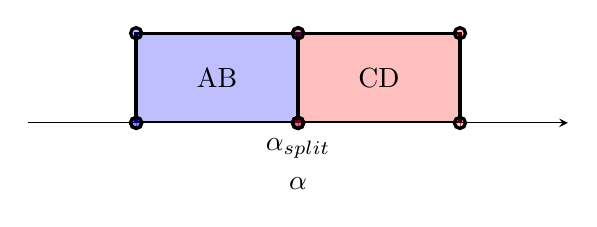
\begin{tikzpicture}
\begin{axis}[
    xmin=0, xmax=1,
    axis x line=bottom,% only show the bottom x axis
    xlabel={$\alpha$},
    xtick={0.2,0.5,0.8},
    xticklabels={$\alo$,$\alpha_{split}$,$\ahi$},
    hide y axis,    
    ymin=0,ymax=5,
    scatter/classes={%
        a={mark=o,draw=black}}
    ]

    \addplot [mark=*,very thick,fill=blue, fill opacity=0.25] coordinates {
        (0.2, 0)
        (0.2, 1)
        (0.5, 1)
        (0.5, 0)
        (0.2, 0)
    };
    \addplot [mark=*,very thick,fill=red, fill opacity=0.25] coordinates {
        (0.5, 0)
        (0.5, 1)
        (0.8, 1)
        (0.8, 0)
        (0.5, 0)
    };
    \node[] at (axis cs: 0.35,0.5) {AB};
    \node[] at (axis cs: 0.65,0.5) {CD};
\end{axis}
\end{tikzpicture}
\end{minipage}
\begin{minipage}{.45\textwidth}
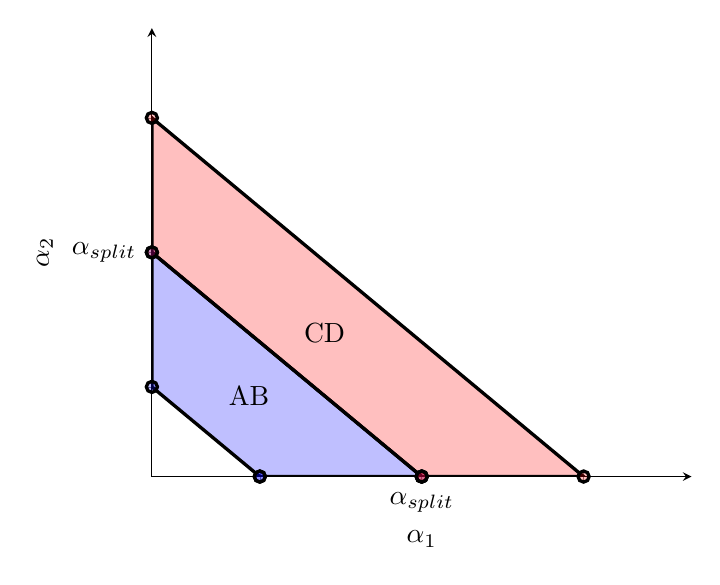
\begin{tikzpicture}
\begin{axis}[
    xmin=0, xmax=1,
    axis x line=bottom,% only show the bottom x axis
    axis y line=left,
    xlabel={$\alpha_1$},
    ylabel={$\alpha_2$},
    xtick={0.2,0.5,0.8},
    xticklabels={$\alo$,$\alpha_{split}$,$\ahi$},  
    ytick={0.2,0.5,0.8},
    yticklabels={$\alo$,$\alpha_{split}$,$\ahi$},  
    ymin=0,ymax=1,
    scatter/classes={%
        a={mark=o,draw=black}}
    ]

    \addplot [mark=*,very thick,fill=blue, fill opacity=0.25] coordinates {
        (0.2, 0)
        (0.5, 0)
        (0, 0.5)
        (0, 0.2)
        (0.2, 0)
    };
    \addplot [mark=*,very thick,fill=red, fill opacity=0.25] coordinates {
        (0.5, 0)
        (0.8, 0)
        (0, 0.8)
        (0, 0.5)
        (0.5, 0)
    };
    \node[] at (axis cs: 0.18,0.18) {AB};
    \node[] at (axis cs: 0.32,0.32) {CD};
\end{axis}
\end{tikzpicture}
\end{minipage}
\caption{While in this work, the split between different merges was based on a linear function $d(\alpha)$ (left), it will be more difficult to evaluate the merges when interpolating with two weight parameters $\alpha_1$ and $\alpha_2$, where the merges will be represented as a convex hull in the $\alpha_1$-$\alpha_2$-space (right).}
\label{fig:convexhull}
\end{figure}

\begin{figure}[h]
\centering
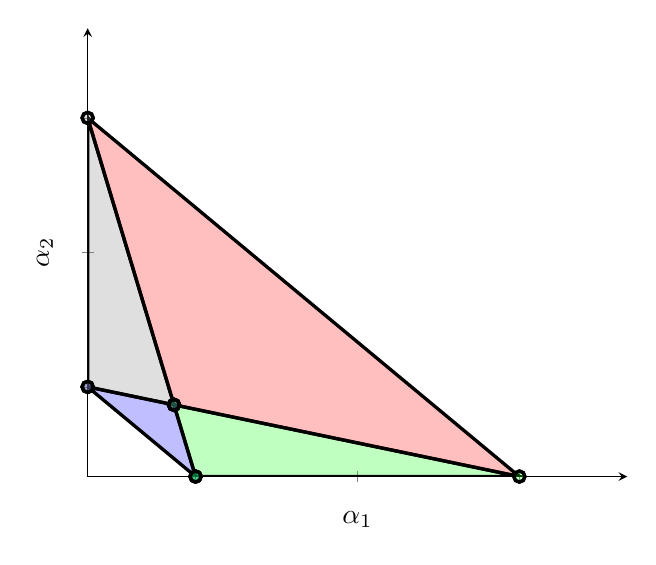
\begin{tikzpicture}
\begin{axis}[
    xmin=0, xmax=1,
    axis x line=bottom,% only show the bottom x axis
    axis y line=left,
    xlabel={$\alpha_1$},
    ylabel={$\alpha_2$},
    xtick={0.2,0.5,0.8},
    xticklabels={$\alo$,,$\ahi$},  
    ytick={0.2,0.5,0.8},
    yticklabels={$\alo$,,$\ahi$},  
    ymin=0,ymax=1,
    scatter/classes={%
        a={mark=o,draw=black}}
    ]
    \addplot [mark=*,very thick,fill=blue, fill opacity=0.25] coordinates {
        (0.2, 0)
        (0, 0.2)
        (0.16, 0.16)
        (0.2, 0)
    };
    \addplot [mark=*,very thick,fill=green, fill opacity=0.25] coordinates {
        (0.2, 0)
        (0.8, 0)
        (0.16, 0.16)
        (0.2, 0)
    };
    \addplot [mark=*,very thick,fill=gray, fill opacity=0.25] coordinates {
        (0, 0.2)
        (0, 0.8)
        (0.16, 0.16)
        (0, 0.2)
    };
    \addplot [mark=o,very thick,fill=red, fill opacity=0.25] coordinates {
        (0.16, 0.16)
        (0.8, 0)
        (0, 0.8)
        (0.16, 0.16)
    };
\end{axis}
\end{tikzpicture}
\caption{Finding the merges in the different regions can be more challenging when interpolating with two weight parameters $\alpha_1$ and $\alpha_2$.}
\label{fig:convexhulls2}
\end{figure}

In addition, we can apply the introduced algorithm to more datasets and data domains, such as the sets contained in the UCI Machine Learning Repository \cite{Dua:2019}. For instance, we could compare different datasets within one specific data domain. Say we evaluate a variety of different image datasets and compare the optimal values of $\alpha$. An interesting observation would be, if we could reuse the optimal parameter from different datasets within the same or even across other domains. In our experiments, we often found similar optimal values in the range $[0.7,0.9]$ while other ranges mostly did not lead to good results (e.g.\ $[0.0, 0.5]$). We could use this knowledge for further experiments by e.g. evaluating only smaller regions or by putting more emphasis on given parameters in general. We can then also evaluate other domains, such as (partially) labeled voice datasets (e.g. the Free Music Archive dataset \cite{fma} or LibriSpeech \cite{librispeech}) and compare the results across different data domains.\\

Also, we can imagine applying this framework to (a) other clustering algorithms than agglomerative hierarchical clustering and (b) other tasks than clustering.

%% --------------------
%% |   Bibliography   |
%% --------------------

%% Add entry to the table of contents for the bibliography
\printbibliography[heading=bibintoc]

%% ----------------
%% |   Appendix   |
%% ----------------
\appendix
\chapter{The Hungarian Method}
\label{sec:hungarian}

Our goal is to find the best possible matching between two clusterings $C_1^i, ..., C_k^i$ and $C_1^j, ..., C_k^j$. In order to do so, we calculate the cost of matching each possible pair of clusters within the two clusterings. 
% Table \ref{app:hung:distances} shows how such a cost matrix can look like.

% \begin{table}[h]
%     \centering
%     \begin{tabular}{|l | l l l l l|}
%     \hline
%     j\textbackslash i & 1 & 2 & 3 & 4 & 5\\ \hline
%     1 & 20 & 15 & 30 & 50 & 40\\
%     2 & 80 & 10 & 15 & 20 & 30\\
%     3 & 20 & 30 & 50 & 80 & 60\\
%     4 & 30 & 50 & 40 & 20 & 10\\
%     5 & 20 & 30 & 40 & 50 & 25\\ \hline
%     \end{tabular}
%     \caption{In order to determine the optimal matching between two clusterings, we note the pairwise matching costs.}
%     \label{app:hung:distances}
% \end{table}

To find the optimal matching in a brute force way, we have to look at each possible matching. Say we want to match each $i$ to one $j$. For $i = 1$ we can pick from 5 different values of $j$, for $i = 2$ there are 4 potential values of $j$. This will overall result in $k! = 5! = 120$ different combinations, thus the complexity of the brute force approach is $O(k!)$. A more efficient algorithm (especially for higher values of $k$) was introduced by Kuhn and Munkres \cite{kuhn1955hungarian}\cite{munkres1957algorithms}. It consists of three major steps. In the first one, we subtract the row minima from each row. This step is performed in table \ref{app:hung:step1}.

\begin{table}[h]
    \centering
    \begin{tabular}{|l | l l l l l| l |}
    \hline
    j\textbackslash i & 1 & 2 & 3 & 4 & 5 & \\ \hline
    1 & 5 & 0 & 15 & 35 & 25 & (-15)\\
    2 & 70 & 0 & 5 & 10 & 20 & (-10)\\
    3 & 0 & 10 & 30 & 60 & 40 & (-20)\\
    4 & 20 & 40 & 30 & 10 & 0 & (-10)\\
    5 & 0 & 10 & 20 & 30 & 5 & (-20)\\ \hline
    \end{tabular}
    \caption{Hungarian method step 1: Subtract the row minima from each row.}
    \label{app:hung:step1}
\end{table}

After subtracting the row minima, we now also subtract the column minima from each column as shown in table \ref{app:hung:step2}.

\begin{table}[h]
    \centering
    \begin{tabular}{|l | l l l l l |}
    \hline
    j\textbackslash i & 1 & 2 & 3 & 4 & 5\\ \hline
    1 & 5 & 0 & 10 & 25 & 25\\
    2 & 70 & 0 & 0 & 0 & 20\\
    3 & 0 & 10 & 25 & 50 & 40\\
    4 & 20 & 40 & 25 & 0 & 0\\
    5 & 0 & 10 & 15 & 20 & 5\\ \hline
    & - & - & (-5) & (-10) & -\\ \hline
    \end{tabular}
    \caption{Hungarian method step 2: Subtract the column minima from each column.}
    \label{app:hung:step2}
\end{table}

Now we try to find the optimal matching. To do so, we cover all zeros with lines and count the minumum needed lines to do so. Table \ref{app:hung:step3} shows that we need four lines.

\begin{table}[h]
    \centering
    \begin{tabular}{|l | l l l l l |}
    \hline
    j\textbackslash i & 1 & 2 & 3 & 4 & 5\\ \hline
    1 & \cellcolor{orange!25}5 & \cellcolor{orange!50}0 & 10 & 25 & 25\\
    2 & \cellcolor{orange!75}70 & \cellcolor{orange!75}0 & \cellcolor{orange!75}0 & \cellcolor{orange!75}0 & \cellcolor{orange!75}20\\
    3 & \cellcolor{orange!25}0 & \cellcolor{orange!50}10 & 25 & 50 & 40\\
    4 & \cellcolor{orange!75}20 & \cellcolor{orange!75}40 & \cellcolor{orange!75}25 & \cellcolor{orange!75}0 & \cellcolor{orange!75}0\\
    5 & \cellcolor{orange!25}0 & \cellcolor{orange!50}10 & 15 & 20 & 5\\ \hline
    \end{tabular}
    \caption{Hungarian method step 3: Cover all zeros with as few lines as possible.}
    \label{app:hung:step3}
\end{table}

After covering the zeros and counting the lines, we found the optimal matching in case the number of lines equals the number of rows (or columns) in the matrix. As we need four lines and the matrix has five rows in this example, we have to add more zeros. To do that, we subtract the minimum value of the matrix (which is 5 here) from all uncovered values that are not zero and add it to all values that are not zero and covered twice. Now we can again check the needed lines as in table \ref{app:hung:additionalstep}.

\begin{table}[h]
    \centering
    \begin{tabular}{|l | l l l l l |}
    \hline
    j\textbackslash i & 1 & 2 & 3 & 4 & 5\\ \hline
    1 & 5 & 0 & 5 & 20 & 20\\
    2 & 75 & 0 & 0 & 0 & 20\\
    3 & 0 & 10 & 20 & 45 & 35\\
    4 & 25 & 45 & 25 & 0 & 0\\
    5 & 0 & 10 & 10 & 15 & 0\\ \hline
    \end{tabular}
    \begin{tabular}{|l | l l l l l |}
        \hline
        j\textbackslash i & 1 & 2 & 3 & 4 & 5\\ \hline
        1 & \cellcolor{orange!25}5 & \cellcolor{orange!50}0 & 5 & 20 & 20\\
        2 & \cellcolor{orange!75}75 & \cellcolor{orange!75}0 & \cellcolor{orange!75}0 & \cellcolor{orange!75}0 & \cellcolor{orange!75}20\\
        3 & \cellcolor{orange!25}0 & \cellcolor{orange!50}10 & 20 & 45 & 35\\
        4 & \cellcolor{orange!75}25 & \cellcolor{orange!75}45 & \cellcolor{orange!75}25 & \cellcolor{orange!75}0 & \cellcolor{orange!75}0\\
        5 & \cellcolor{orange!100}0 & \cellcolor{orange!100}10 & \cellcolor{orange!100}10 & \cellcolor{orange!100}15 & \cellcolor{orange!100}0\\ \hline
    \end{tabular}
    \caption{Hungarian method additional step: Create more zeroes until the number of minimal needed lines to cover all zeros matches the number of rows.}
    \label{app:hung:additionalstep}
\end{table}

This will then result in the assignment seen in table \ref{app:hung:assignment}. Applying the matching to the input matrix then gives the optimal cost by summing the optimal values. For this example the optimal cost is then 95.

\begin{table}[h]
    \centering
    \begin{tabular}{|l | l l l l l |}
    \hline
    j\textbackslash i & 1 & 2 & 3 & 4 & 5\\ \hline
    1 & 5 & \cellcolor{blue!25}0 & 5 & 20 & 20\\
    2 & 75 & 0 & \cellcolor{blue!25}0 & 0 & 20\\
    3 & \cellcolor{blue!25}0 & 10 & 20 & 45 & 35\\
    4 & 25 & 45 & 25 & \cellcolor{blue!25}0 & 0\\
    5 & 0 & 10 & 10 & 15 & \cellcolor{blue!25}0\\ \hline
    \end{tabular}
    \begin{tabular}{|l | l l l l l|}
        \hline
        j\textbackslash i & 1 & 2 & 3 & 4 & 5\\ \hline
        1 & 20 & \cellcolor{blue!25}15 & 30 & 50 & 40\\
        2 & 80 & 10 & \cellcolor{blue!25}15 & 20 & 30\\
        3 & \cellcolor{blue!25}20 & 30 & 50 & 80 & 60\\
        4 & 30 & 50 & 40 & \cellcolor{blue!25}20 & 10\\
        5 & 20 & 30 & 40 & 50 & \cellcolor{blue!25}25\\ \hline
    \end{tabular}
    \caption{Result of the Hungarian method: The optimal matching between two clusterings.}
    \label{app:hung:assignment}
\end{table}	% Appendix Title

\chapter{Convolutional Neural Network Architecture for Feature Extraction}
\label{sec:cnnarchitecture}

\begin{figure}[H]
    \centering
    \includegraphics[width=0.6\textwidth]{images/model}
    \caption{We use a small Convolutional Neural Network (CNN) architecture to create meaningful features for the MNIST and the Omniglot data.}
    \label{fig:model}
\end{figure} % Appendix Title

\chapter{Additional NELL Results}
\label{app:nell}

Here we show the results of all the 30 different used entities. We used a maximum of 1,000 points for each entity, however for some of them less samples were given. We show both interpolating between average and complete and between single and complete linkage in the following figures.

\begin{figure}[h]
\centering
\begin{minipage}{.24\textwidth}
  \centering
  \subcaptionbox{Animal}
  {\includegraphics[width=\linewidth]{plots/nell-ac/animal}}
\end{minipage}
\begin{minipage}{.24\textwidth}
  \centering
  \subcaptionbox{Arthropod}
  {\includegraphics[width=\linewidth]{plots/nell-ac/arthropod}}
\end{minipage}
\begin{minipage}{.24\textwidth}
  \centering
  \subcaptionbox{Attraction}
  {\includegraphics[width=\linewidth]{plots/nell-ac/attraction}}
\end{minipage}
\begin{minipage}{.24\textwidth}
  \centering
  \subcaptionbox{Beverage}
  {\includegraphics[width=\linewidth]{plots/nell-ac/beverage}}
\end{minipage}
\begin{minipage}{.24\textwidth}
  \centering
  \subcaptionbox{Bodypart}
  {\includegraphics[width=\linewidth]{plots/nell-ac/bodypart}}
\end{minipage}
\begin{minipage}{.24\textwidth}
  \centering
  \subcaptionbox{Building}
  {\includegraphics[width=\linewidth]{plots/nell-ac/building}}
\end{minipage}
\begin{minipage}{.24\textwidth}
  \centering
  \subcaptionbox{Company}
  {\includegraphics[width=\linewidth]{plots/nell-ac/company}}
\end{minipage}
\begin{minipage}{.24\textwidth}
  \centering
  \subcaptionbox{Creative Work}
  {\includegraphics[width=\linewidth]{plots/nell-ac/creativework}}
\end{minipage}
\begin{minipage}{.24\textwidth}
  \centering
  \subcaptionbox{Date}
  {\includegraphics[width=\linewidth]{plots/nell-ac/date}}
\end{minipage}
\begin{minipage}{.24\textwidth}
  \centering
  \subcaptionbox{Event}
  {\includegraphics[width=\linewidth]{plots/nell-ac/event}}
\end{minipage}
\begin{minipage}{.24\textwidth}
  \centering
  \subcaptionbox{Food}
  {\includegraphics[width=\linewidth]{plots/nell-ac/food}}
\end{minipage}
\begin{minipage}{.24\textwidth}
  \centering
  \subcaptionbox{Fruit}
  {\includegraphics[width=\linewidth]{plots/nell-ac/fruit}}
\end{minipage}
\begin{minipage}{.24\textwidth}
  \centering
  \subcaptionbox{Game}
  {\includegraphics[width=\linewidth]{plots/nell-ac/game}}
\end{minipage}
\begin{minipage}{.24\textwidth}
  \centering
  \subcaptionbox{Household Item}
  {\includegraphics[width=\linewidth]{plots/nell-ac/householditem}}
\end{minipage}
\begin{minipage}{.24\textwidth}
  \centering
  \subcaptionbox{Invertebrate}
  {\includegraphics[width=\linewidth]{plots/nell-ac/invertebrate}}
\end{minipage}
\begin{minipage}{.24\textwidth}
  \centering
  \subcaptionbox{Location}
  {\includegraphics[width=\linewidth]{plots/nell-ac/location}}
\end{minipage}
\end{figure}
\begin{figure}[h]\ContinuedFloat
\centering
\begin{minipage}{.24\textwidth}
  \centering
  \subcaptionbox{Mediacompany}
  {\includegraphics[width=\linewidth]{plots/nell-ac/mediacompany}}
\end{minipage}
\begin{minipage}{.24\textwidth}
  \centering
  \subcaptionbox{Organization}
  {\includegraphics[width=\linewidth]{plots/nell-ac/organization}}
\end{minipage}
\begin{minipage}{.24\textwidth}
  \centering
  \subcaptionbox{Person}
  {\includegraphics[width=\linewidth]{plots/nell-ac/person}}
\end{minipage}
\begin{minipage}{.24\textwidth}
  \centering
  \subcaptionbox{Person by Location}
  {\includegraphics[width=\linewidth]{plots/nell-ac/personbylocation}}
\end{minipage}
\begin{minipage}{.24\textwidth}
  \centering
  \subcaptionbox{Person NA}
  {\includegraphics[width=\linewidth]{plots/nell-ac/personnorthamerica}}
\end{minipage}
\begin{minipage}{.24\textwidth}
  \centering
  \subcaptionbox{Physiological Condition}
  {\includegraphics[width=\linewidth]{plots/nell-ac/physiologicalcondition}}
\end{minipage}
\begin{minipage}{.24\textwidth}
  \centering
  \subcaptionbox{Politics Group}
  {\includegraphics[width=\linewidth]{plots/nell-ac/politicsgroup}}
\end{minipage}
\begin{minipage}{.24\textwidth}
  \centering
  \subcaptionbox{Product}
  {\includegraphics[width=\linewidth]{plots/nell-ac/Product}}
\end{minipage}
\begin{minipage}{.24\textwidth}
  \centering
  \subcaptionbox{Publication}
  {\includegraphics[width=\linewidth]{plots/nell-ac/publication}}
\end{minipage}
\begin{minipage}{.24\textwidth}
  \centering
  \subcaptionbox{School}
  {\includegraphics[width=\linewidth]{plots/nell-ac/school}}
\end{minipage}
\begin{minipage}{.24\textwidth}
  \centering
  \subcaptionbox{Software}
  {\includegraphics[width=\linewidth]{plots/nell-ac/software}}
\end{minipage}
\begin{minipage}{.24\textwidth}
  \centering
  \subcaptionbox{Sports Event}
  {\includegraphics[width=\linewidth]{plots/nell-ac/sportsevent}}
\end{minipage}
\begin{minipage}{.24\textwidth}
  \centering
  \subcaptionbox{Traditional Game}
  {\includegraphics[width=\linewidth]{plots/nell-ac/traditionalgame}}
\end{minipage}
\begin{minipage}{.24\textwidth}
  \centering
  \subcaptionbox{Vertebrate}
  {\includegraphics[width=\linewidth]{plots/nell-ac/vertebrate}}
\end{minipage}
\begin{minipage}{.24\textwidth}
  \centering
  \subcaptionbox{Visualizable Attribute}
  {\includegraphics[width=\linewidth]{plots/nell-ac/visualizableattribute}}
\end{minipage}
\begin{minipage}{.24\textwidth}
  \centering
  \subcaptionbox{Website}
  {\includegraphics[width=\linewidth]{plots/nell-ac/website}}
\end{minipage}
\caption{Interpolating between average and complete linkage for the NELL data.}
\end{figure}

\begin{figure}[h]
\centering
\begin{minipage}{.24\textwidth}
  \centering
  \subcaptionbox{Animal}
  {\includegraphics[width=\linewidth]{plots/nell-sc/animal}}
\end{minipage}
\begin{minipage}{.24\textwidth}
  \centering
  \subcaptionbox{Arthropod}
  {\includegraphics[width=\linewidth]{plots/nell-sc/arthropod}}
\end{minipage}
\begin{minipage}{.24\textwidth}
  \centering
  \subcaptionbox{Attraction}
  {\includegraphics[width=\linewidth]{plots/nell-sc/attraction}}
\end{minipage}
\begin{minipage}{.24\textwidth}
  \centering
  \subcaptionbox{Beverage}
  {\includegraphics[width=\linewidth]{plots/nell-sc/beverage}}
\end{minipage}
\begin{minipage}{.24\textwidth}
  \centering
  \subcaptionbox{Bodypart}
  {\includegraphics[width=\linewidth]{plots/nell-sc/bodypart}}
\end{minipage}
\begin{minipage}{.24\textwidth}
  \centering
  \subcaptionbox{Building}
  {\includegraphics[width=\linewidth]{plots/nell-sc/building}}
\end{minipage}
\begin{minipage}{.24\textwidth}
  \centering
  \subcaptionbox{Company}
  {\includegraphics[width=\linewidth]{plots/nell-sc/company}}
\end{minipage}
\begin{minipage}{.24\textwidth}
  \centering
  \subcaptionbox{Creative Work}
  {\includegraphics[width=\linewidth]{plots/nell-sc/creativework}}
\end{minipage}
\begin{minipage}{.24\textwidth}
  \centering
  \subcaptionbox{Date}
  {\includegraphics[width=\linewidth]{plots/nell-sc/date}}
\end{minipage}
\begin{minipage}{.24\textwidth}
  \centering
  \subcaptionbox{Event}
  {\includegraphics[width=\linewidth]{plots/nell-sc/event}}
\end{minipage}
\begin{minipage}{.24\textwidth}
  \centering
  \subcaptionbox{Food}
  {\includegraphics[width=\linewidth]{plots/nell-sc/food}}
\end{minipage}
\begin{minipage}{.24\textwidth}
  \centering
  \subcaptionbox{Fruit}
  {\includegraphics[width=\linewidth]{plots/nell-sc/fruit}}
\end{minipage}
\begin{minipage}{.24\textwidth}
  \centering
  \subcaptionbox{Game}
  {\includegraphics[width=\linewidth]{plots/nell-sc/game}}
\end{minipage}
\begin{minipage}{.24\textwidth}
  \centering
  \subcaptionbox{Household Item}
  {\includegraphics[width=\linewidth]{plots/nell-sc/householditem}}
\end{minipage}
\begin{minipage}{.24\textwidth}
  \centering
  \subcaptionbox{Invertebrate}
  {\includegraphics[width=\linewidth]{plots/nell-sc/invertebrate}}
\end{minipage}
\begin{minipage}{.24\textwidth}
  \centering
  \subcaptionbox{Location}
  {\includegraphics[width=\linewidth]{plots/nell-sc/location}}
\end{minipage}
\begin{minipage}{.24\textwidth}
  \centering
  \subcaptionbox{Mediacompany}
  {\includegraphics[width=\linewidth]{plots/nell-sc/mediacompany}}
\end{minipage}
\begin{minipage}{.24\textwidth}
  \centering
  \subcaptionbox{Organization}
  {\includegraphics[width=\linewidth]{plots/nell-sc/organization}}
\end{minipage}
\begin{minipage}{.24\textwidth}
  \centering
  \subcaptionbox{Person}
  {\includegraphics[width=\linewidth]{plots/nell-sc/person}}
\end{minipage}
\begin{minipage}{.24\textwidth}
  \centering
  \subcaptionbox{Person by Location}
  {\includegraphics[width=\linewidth]{plots/nell-sc/personbylocation}}
\end{minipage}
\end{figure}
\begin{figure}[h]\ContinuedFloat
\centering
\begin{minipage}{.24\textwidth}
  \centering
  \subcaptionbox{Person NA}
  {\includegraphics[width=\linewidth]{plots/nell-sc/personnorthamerica}}
\end{minipage}
\begin{minipage}{.24\textwidth}
  \centering
  \subcaptionbox{Physiological Condition}
  {\includegraphics[width=\linewidth]{plots/nell-sc/physiologicalcondition}}
\end{minipage}
\begin{minipage}{.24\textwidth}
  \centering
  \subcaptionbox{Politics Group}
  {\includegraphics[width=\linewidth]{plots/nell-sc/politicsgroup}}
\end{minipage}
\begin{minipage}{.24\textwidth}
  \centering
  \subcaptionbox{Product}
  {\includegraphics[width=\linewidth]{plots/nell-sc/Product}}
\end{minipage}
\begin{minipage}{.24\textwidth}
  \centering
  \subcaptionbox{Publication}
  {\includegraphics[width=\linewidth]{plots/nell-sc/publication}}
\end{minipage}
\begin{minipage}{.24\textwidth}
  \centering
  \subcaptionbox{School}
  {\includegraphics[width=\linewidth]{plots/nell-sc/school}}
\end{minipage}
\begin{minipage}{.24\textwidth}
  \centering
  \subcaptionbox{Software}
  {\includegraphics[width=\linewidth]{plots/nell-sc/software}}
\end{minipage}
\begin{minipage}{.24\textwidth}
  \centering
  \subcaptionbox{Sports Event}
  {\includegraphics[width=\linewidth]{plots/nell-sc/sportsevent}}
\end{minipage}
\begin{minipage}{.24\textwidth}
  \centering
  \subcaptionbox{Traditional Game}
  {\includegraphics[width=\linewidth]{plots/nell-sc/traditionalgame}}
\end{minipage}
\begin{minipage}{.24\textwidth}
  \centering
  \subcaptionbox{Vertebrate}
  {\includegraphics[width=\linewidth]{plots/nell-sc/vertebrate}}
\end{minipage}
\begin{minipage}{.24\textwidth}
  \centering
  \subcaptionbox{Visualizable Attribute}
  {\includegraphics[width=\linewidth]{plots/nell-sc/visualizableattribute}}
\end{minipage}
\begin{minipage}{.24\textwidth}
  \centering
  \subcaptionbox{Website}
  {\includegraphics[width=\linewidth]{plots/nell-sc/website}}
\end{minipage}
\caption{Interpolating between single and complete linkage for the NELL data.}
\end{figure} % Appendix Title

\end{document}



% %% ----------------------------------------------------------------
% %% Thesis.tex -- MAIN FILE (the one that you compile with LaTeX)
% %% ---------------------------------------------------------------- 

% % Set up the document
% \documentclass[a4paper, 11pt, oneside]{Thesis}  % Use the "Thesis" style, based on the ECS Thesis style by Steve Gunn
% \graphicspath{Figures/}  % Location of the graphics files (set up for graphics to be in PDF format)

% % Include any extra LaTeX packages required


% %% ----------------------------------------------------------------
% \begin{document}
% \frontmatter      % Begin Roman style (i, ii, iii, iv...) page numbering

% % Set up the Title Page
% \title  {Data‒driven learning of clustering algorithms for text and image data}
% \authors  {\texorpdfstring
%             {\href{your web site or email address}{Manuel Lang}}
%             {Manuel Lang}
%             }
% \addresses  {\groupname\\\deptname\\\univname}  % Do not change this here, instead these must be set in the "Thesis.cls" file, please look through it instead
% \date       {\today}
% \subject    {}
% \keywords   {}

% %\maketitle
% %% ----------------------------------------------------------------

% \setstretch{1.3}  % It is better to have smaller font and larger line spacing than the other way round

% % Define the page headers using the FancyHdr package and set up for one-sided printing
% \fancyhead{}  % Clears all page headers and footers
% \rhead{\thepage}  % Sets the right side header to show the page number
% \lhead{}  % Clears the left side page header

% \pagestyle{fancy}  % Finally, use the "fancy" page style to implement the FancyHdr headers

% %% ----------------------------------------------------------------
% % Declaration Page required for the Thesis, your institution may give you a different text to place here
% % \Declaration{

% % \addtocontents{toc}{\vspace{1em}}  % Add a gap in the Contents, for aesthetics

% % I, AUTHOR NAME, declare that this thesis titled, `THESIS TITLE' and the work presented in it are my own. I confirm that:

% % \begin{itemize} 
% % \item[\tiny{$\blacksquare$}] This work was done wholly or mainly while in candidature for a research degree at this University.
 
% % \item[\tiny{$\blacksquare$}] Where any part of this thesis has previously been submitted for a degree or any other qualification at this University or any other institution, this has been clearly stated.
 
% % \item[\tiny{$\blacksquare$}] Where I have consulted the published work of others, this is always clearly attributed.
 
% % \item[\tiny{$\blacksquare$}] Where I have quoted from the work of others, the source is always given. With the exception of such quotations, this thesis is entirely my own work.
 
% % \item[\tiny{$\blacksquare$}] I have acknowledged all main sources of help.
 
% % \item[\tiny{$\blacksquare$}] Where the thesis is based on work done by myself jointly with others, I have made clear exactly what was done by others and what I have contributed myself.
% % \\
% % \end{itemize}
 
 
% % Signed:\\
% % \rule[1em]{25em}{0.5pt}  % This prints a line for the signature
 
% % Date:\\
% % \rule[1em]{25em}{0.5pt}  % This prints a line to write the date
% % }
% % \clearpage  % Declaration ended, now start a new page

% %% ----------------------------------------------------------------
% % The "Funny Quote Page"
% % \pagestyle{empty}  % No headers or footers for the following pages

% % \null\vfill
% % % Now comes the "Funny Quote", written in italics
% % \textit{``Write a funny quote here.''}

% % \begin{flushright}
% % If the quote is taken from someone, their name goes here
% % \end{flushright}

% % \vfill\vfill\vfill\vfill\vfill\vfill\null
% % \clearpage  % Funny Quote page ended, start a new page
% %% ----------------------------------------------------------------

% % The Abstract Page
% % \addtotoc{Abstract}  % Add the "Abstract" page entry to the Contents
% % \abstract{
% % \addtocontents{toc}{\vspace{1em}}  % Add a gap in the Contents, for aesthetics

% % The Thesis Abstract is written here (and usually kept to just this page). The page is kept centered vertically so can expand into the blank space above the title too\ldots

% % }

%  \clearpage  % Abstract ended, start a new page
% %% ----------------------------------------------------------------

%  \setstretch{1.3}  % Reset the line-spacing to 1.3 for body text (if it has changed)

% % % The Acknowledgements page, for thanking everyone
% % \acknowledgements{
% % \addtocontents{toc}{\vspace{1em}}  % Add a gap in the Contents, for aesthetics

% % The acknowledgements and the people to thank go here, don't forget to include your project advisor\ldots

% % }
% % \clearpage  % End of the Acknowledgements
% %% ----------------------------------------------------------------

% \pagestyle{fancy}  %The page style headers have been "empty" all this time, now use the "fancy" headers as defined before to bring them back


% %% ----------------------------------------------------------------
% \lhead{\emph{Contents}}  % Set the left side page header to "Contents"
% \tableofcontents  % Write out the Table of Contents

% %% ----------------------------------------------------------------
%  \lhead{\emph{List of Figures}}  % Set the left side page header to "List if Figures"
%  \listoffigures  % Write out the List of Figures

% %% ----------------------------------------------------------------
%  \lhead{\emph{List of Tables}}  % Set the left side page header to "List of Tables"
%  \listoftables  % Write out the List of Tables

% %% ----------------------------------------------------------------
% % \setstretch{1.5}  % Set the line spacing to 1.5, this makes the following tables easier to read
% % \clearpage  % Start a new page
% % \lhead{\emph{Abbreviations}}  % Set the left side page header to "Abbreviations"
% % \listofsymbols{ll}  % Include a list of Abbreviations (a table of two columns)
% % {
% % % \textbf{Acronym} & \textbf{W}hat (it) \textbf{S}tands \textbf{F}or \\
% % \textbf{LAH} & \textbf{L}ist \textbf{A}bbreviations \textbf{H}ere \\

% % }

% %% ----------------------------------------------------------------
% % \clearpage  % Start a new page
% % \lhead{\emph{Physical Constants}}  % Set the left side page header to "Physical Constants"
% % \listofconstants{lrcl}  % Include a list of Physical Constants (a four column table)
% % {
% % % Constant Name & Symbol & = & Constant Value (with units) \\
% % Speed of Light & $c$ & $=$ & $2.997\ 924\ 58\times10^{8}\ \mbox{ms}^{-\mbox{s}}$ (exact)\\

% % }

% %% ----------------------------------------------------------------
% % \clearpage  %Start a new page
% % \lhead{\emph{Symbols}}  % Set the left side page header to "Symbols"
% % \listofnomenclature{lll}  % Include a list of Symbols (a three column table)
% % {
% % % symbol & name & unit \\
% % $a$ & distance & m \\
% % $P$ & power & W (Js$^{-1}$) \\
% % & & \\ % Gap to separate the Roman symbols from the Greek
% % $\omega$ & angular frequency & rads$^{-1}$ \\
% % }
% %% ----------------------------------------------------------------
% % End of the pre-able, contents and lists of things
% % Begin the Dedication page

% % \setstretch{1.3}  % Return the line spacing back to 1.3

% % \pagestyle{empty}  % Page style needs to be empty for this page
% % \dedicatory{For/Dedicated to/To my\ldots}

% % \addtocontents{toc}{\vspace{2em}}  % Add a gap in the Contents, for aesthetics


% %% ----------------------------------------------------------------
% \mainmatter	  % Begin normal, numeric (1,2,3...) page numbering
% \pagestyle{fancy}  % Return the page headers back to the "fancy" style

% % Include the chapters of the thesis, as separate files
% % Just uncomment the lines as you write the chapters

% \chapter{Introduction}


Unsupervised grouping is used in various applications to categorize data observations into similar regions. As an example, similar documents can be combined into clusters so that for a new document or a search query, a list of corresponding documents can be suggested \cite{zamir1998web}. The same procedure can also be applied for different tasks, such as grouping products \cite{balakrishnan2018product}, searching images \cite{lin2018dimensionality} or detecting anomalies \cite{he2003discovering}. In comparison to supervised learning, the data does not must be (completely) annotated, i.e.\ potentially expensive labeling work can be omitted by using clustering algorithms. This benefit is one of the reasons why leading researchers think that unsupervised learning will be very important in the future. AI researcher and professor at NYU, Yann LeCun, wrote the following on his personal Facebook profile emphasizing the importance of unsupervised learning methods:

\blockquote{``Most of human and animal learning is unsupervised learning. If intelligence was a cake, unsupervised learning would be the cake, supervised learning would be the icing on the cake, and reinforcement learning would be the cherry on the cake. We know how to make the icing and the cherry, but we don’t know how to make the cake. We need to solve the unsupervised learning problem before we can even think of getting to true AI \cite{lecun}.''}

As the amount of available data has been increasing in the past \cite{wamba2015big}, data analysis is more often required. State-of-the-art algorithms mostly provide general complexity and runtime guarantees. Thus, worst-case guarantees have to be assumed for the given dataset. However, as large datasets do often not adapt much over time, it is very likely that also runtime and complexity of certain algorithms applied to the given data will not change much. On the other hand, it is not trivial which algorithm can then be used to obtain the optimal results, i.e.\ the optimal clusters of the given data \cite{DBLP:journals/corr/GuptaR15b}.\\

In addition, data is often split into different natural representations. For instance, images can be seen as a matrix of pixels, but also with a textual description. For machine learning experiments, it can be difficult to create a model based on various representations as it does not seem intuitive how to stack different data sources such as pixels and textual descriptions \cite{cebral2018combining}.\\

This thesis proposes several algorithms to efficiently use a linear combination of clustering algorithms to overcome the hurdle of selecting the proper algorithm for the given data. In addition, the framework this algorithm is built in\footnote{The implementation is published open-source, see \url{https://github.com/manu183/Learning-to-Link}.} will also be applied to learning a weighted linear combination of feature representations. The proposed clustering algorithms belong to a specific family that will be introduced in chapter \ref{chapter:relatedwork}. % Introduction

% \chapter{Background Theory}
\label{chapter:background}

\section{Data-driven Algorithm Design}

This increasing amount of data allows us to improve the learning capabilities of machines. We know how well existing algorithms perform in general and which runtime guarantees they have. However, the algorithms' guarantees are general observations and can vary a lot between different data. Also, it is often not trivial to choose the right algorithm for the given data without extensive data engineering. In many real-world applications the data does not vary that much, e.g.\ the data for clustering websites into different types may vary quite much on a yearly base, but as this task can get executed thousands of times each second for certain search algorithms, the data will not change much. By assuming a static context, it is then possible to leverage the context to improve the algorithmic results, e.g.\ say you want to cluster person data for different genders. By having this a-priori information, you can use a k-means clustering algorithm with $k = 3$ in order to differentiate between female, male and non-binary people.\\

However, such observations are mostly not that trivial and often require more effort in order to obtain useful a-priori information. In order to cluster financial standing, one could imagine seeing different clusters depending on the age or the education. But how many clusters would result here? The data has to be processed and evaluated for different values in this case.\\

Once our algorithm performs well for our data and our tasks, we then want to transfer the gained knowledge to different tasks. Say the algorithm already learned how to differentiate images of the handwritten digits zero, one and two, the same algorithm should then be able to apply the gained knowledge to distinguish between other handwritten digits too. The gained knowledge is some kind of learned data, that can for example be the feature representation of a Convolutional Neural Network, where a potential goal can be to transfer the representation knowledge to another classification task.\\

For clustering tasks learned knowledge could be a number of clusters, a good feature representation for the input data or other useful information that allows performing similar clustering tasks better by transferring the knowledge.

\section{Linkage-based hierarchical clustering.}

This thesis focuses on agglomerative hierarchical clustering, i.e.\ clustering algorithms that merge clusters starting from each cluster as its own point until all points belong to the same cluster. In each iteration, the two clusters with the closest distance get merged together. As there are various clustering algorithms, there also are various distance measurements. One way to describe the distance between two clusters, say $X$ and $Y$, is by defining a linkage between them. There are three main methods to do so \cite{Manning:2008:IIR:1394399}.

\paragraph{Single Linkage.}

Single linkage defines a distance between two clusters $X$ and $Y$ as the distance between the two nearest points of these clusters (see equation \ref{eq:singlelinkage}).

\begin{equation}
    \begin{aligned}
        d_{SL}(X,Y) = \min\limits_{x \in X, y \in Y} d(x,y)
    \end{aligned}
    \label{eq:singlelinkage}
\end{equation}

\paragraph{Complete Linkage.}

Complete linkage defines a distance between two clusters $X$ and $Y$ as the distance between the two farthest points of these clusters (see equation \ref{eq:completelinkage}).

\begin{equation}
    \begin{aligned}
        d_{CL}(X,Y) = \max\limits_{x \in X, y \in Y} d(x,y)
    \end{aligned}
    \label{eq:completelinkage}
\end{equation}

\paragraph{Average Linkage.}

Average linkage defines a distance between two clusters $X$ and $Y$ as the average distance between all points $x \in X$ and all points $y \in Y$ (see equation \ref{eq:averagelinkage}).

\begin{equation}
    \begin{aligned}
        d_{AL}(X,Y) = \frac{1}{|X||Y|}\sum\limits_{x \in X, y \in Y} d(x,y)
    \end{aligned}
    \label{eq:averagelinkage}
\end{equation}

Figure \ref{fig:linkage_types} demonstrates which points are used for the different linkage strategies using two exemplary clusters.

\begin{figure}[h]
    \centering
    \includegraphics[width=0.8\textwidth]{images/linkage_types}
    \caption{To calculate the distance between two clusters, single linkage calculates the nearest neighbor distance, complete linkage uses the farthest neighbor and average linkage calculates the average distance over all points \cite{linkage_types}.}
    \label{fig:linkage_types}
\end{figure}

\paragraph{Effects of different linkage strategies.}

Depending on the linkage strategy, the pairwise distances between all $N$ clusters $C_1, ..., C_N$ will be different. As the clustering algorithm merges the closest pair of clusters in each iteration, the merging clusters $C_i$ and $C_j$ with $i, j \in 1,...,N$ might vary as shown in figure \ref{fig:linkage_effects}, where ten clusters $C_0, ..., C_9$ get clustered with bottom-up hierarchical clustering using the Euclidean distance as the pointwise distance $d(x,y)$ to calculate the pairwise distance according to the three mentioned linkage strategies.

\begin{figure}[h]
    \centering
    \includegraphics[width=0.8\textwidth]{images/linkage_effects}
    \caption{Different distance measurements often result in different merges for bottom-up hierarchical clustering algorithms. The three discussed linkage strategies result in three different clusterings.}
    \label{fig:linkage_effects}
\end{figure}

As different points are merged together, this also means that the clustering may have a different quality. This thesis compares the clusterings' quality for different data by introducing algorithms to efficiently determine the quality not only for these linkage strategies but also for their linear combinations.

\section{Generating Feature Representations}

In order to improve the overall clustering performance, this work uses several techniques to obtain better feature representations of text and image data. 

\subsection{Text Features}

To cluster different words, there are several ways to create a difference measurement of these words. 

\paragraph{Word Edit Distance.} A rather simple approach would be to calculate the edit distance that describes the difference of the characters in the words \cite{ristad1998learning}. However, this approach does not contain any semantic information, i.e.\ synonyms will have a larger distance than wanted. For example the edit distance between loan and moan is very small ($wed(loan, moan) = 1$) where the edit distance between loan and credit is larger ($wed(loan, credit) = 6)$.\\ 

\paragraph{Word Embeddings.} This motivates to leverage contextual information, where we can use several pre-trained models on different datasets. Stanford's GloVe provides such models that incorporate knowledge from Wikipedia and social networks \cite{pennington2014glove}. Figure \ref{fig:glove} shows examples for why these embeddings give a helpful feature representation.\\

\begin{figure}[h]
\centering
\begin{minipage}{.3\textwidth}
  \centering
  \includegraphics[width=\linewidth]{images/glove_mw}
\end{minipage}
\begin{minipage}{.3\textwidth}
  \centering
  \includegraphics[width=\linewidth]{images/glove_cz}
\end{minipage}
\begin{minipage}{.3\textwidth}
  \centering
  \includegraphics[width=\linewidth]{images/glove_cs}
\end{minipage}
\caption{Word embeddings give insightful correlations between similar and different words. For example, we can obtain several relations between female and male people, between zip codes and cities or between comparative and superlative words \cite{pennington2014glove}.}
\label{fig:glove}
\end{figure}

\paragraph{Bag of Contexts.} In addition, CMU's Machine Learning Department provides another way to compare words. Their Never-Ending Language Learner provides information in which contexts certain words are used online \cite{nell_pairs}, e.g.\ by considering that both Pittsburgh and Karlsruhe are used in the one same context ``is a city'' and Pittsburgh and Philadelphia share additional contexts such as ``belongs to the state Pennsylvania'', we can conclude that Pittsburgh has a higher correlation to Philadelphia than to Karlsruhe. We can then create a corpus containing all different contexts. Similar to the bag-of-words approach, we can then count the occurrences of the words in the corpus' contexts. However, the resulting data is very sparse and Euclidean distance will not work well to compare the ``bag-of-contexts'' representations, i.e.\ other measurements such as the cosine distance are preferred.

\subsection{Image Features}
\label{sec:imagefeatures}

Similarly, there also exist ways to extract useful features from image data. In particular, this work focuses on neutral networks that learn to represent images in a way that images of different classes can be seperated well where images of the same class might share similar features.\\

\paragraph{CNN Features.} As a primary example, we use Convolutional Neural Network (CNN) architectures that learn to represent images with convolutional, pooling and activation layers and later map the representations to target classes with fully-connected layers. In this way, we can cut off the fully-connected layers to extract lower-dimensional feature representations for the input image data. Figure \ref{fig:cnnfeatures} visualizes such features learned on the ImageNet dataset \cite{krizhevsky2012imagenet}.

\begin{figure}[h]
    \centering
    \includegraphics[width=0.8\textwidth]{images/cnn_features}
    \caption{Convolutional Neural Networks learn to represent images in lower-dimensional feature maps by applying convolutions to the image and averaging local neighborhoods (pooling) \cite{krizhevsky2012imagenet}.}
    \label{fig:cnnfeatures}
\end{figure} % Background Theory 

% \chapter{Related Work}
\label{chapter:relatedwork}

\section{Data-driven Algorithm Design}

We know how well existing algorithms perform in general and which complexity guarantees they have. However, the algorithms' guarantees are general observations and can vary a lot between different data. Also, it is often not trivial to choose the right algorithm for the given data without extensive data engineering. In many real-world applications, the data does not vary that much. For instance, the data for clustering websites into different types may vary quite much on a yearly base, but as this task can get executed thousands of times each second for certain search algorithms, the data will not change much. By assuming a static context, it is then possible to leverage the context to improve the algorithmic results. Empirical work without much theoretical foundation exists in domains such as artificial intelligence \cite{Xu:2008:SPA:1622673.1622687}, computational biology \cite{deblasio2018adaptive} or game theory \cite{likhodedov2004methods}. However, in this work we focus on clustering tasks, e.g.\ say we want to cluster person data for different genders. By having apriori information, we can use a k-means clustering algorithm with $k = 3$ in order to differentiate between female, male and non-binary people.\\

However, such observations are mostly not trivial and often require more effort in order to obtain useful apriori information. In order to cluster financial standing, one could imagine seeing different clusters depending on the age or the education. But how many clusters would result here? The data has to be processed and evaluated for different values in this case.\\

Once our algorithm performs well for our data and our tasks, we then want to transfer the gained knowledge to different tasks. Say the algorithm has already learned how to differentiate images of the handwritten digits zero, one and two, the same algorithm should then be able to apply the gained knowledge to distinguish between other handwritten digits too. The gained knowledge is some kind of learned data, that for example can be the feature representation of a Convolutional Neural Network, where a potential goal can be to transfer the representation knowledge to another classification task. For clustering tasks learned knowledge could be a number of clusters, a good feature representation for the input data or other useful information that allows performing similar clustering tasks better by transferring the knowledge.\\

Data-driven learning is in general closely related to hyperparameter tuning \cite{hutter2015beyond}, where we try to find the best value of a given parameter to optimize the overall quality, automated machine learning \cite{lacoste2014sequential,liu2018very}, where we perform end-to-end learning for given data, and meta learning \cite{alexandros2001model}, where we try to extract meta-knowledge as one step of the learning process.

\section{Linkage-based Hierarchical Clustering}

This thesis focuses on agglomerative hierarchical clustering, i.e.\ clustering algorithms that merge clusters starting from each point as its own cluster until all points belong to the same cluster. In each iteration, the two clusters with the closest distance get merged together. As there are various clustering algorithms, there are also various distance measurements which are widely used in practice and optimal in many cases \cite{awasthi2017local,saeed2003software,white2010alignment,awasthi2012center,balcan2016clustering,grosswendt2017improved}. One popular way to describe the distance between two clusters is by defining a linkage between them. There are three main methods to do so \cite{Manning:2008:IIR:1394399}.

\paragraph{Single Linkage.}

Single linkage defines a distance between two clusters $X$ and $Y$ as the distance between the two nearest points of these clusters.

\begin{equation*}
    \begin{aligned}
        d_{SL}(X,Y) = \min\limits_{x \in X, y \in Y} d(x,y)
    \end{aligned}
    \label{eq:singlelinkage}
\end{equation*}

\paragraph{Complete Linkage.}

Complete linkage defines a distance between two clusters $X$ and $Y$ as the distance between the two farthest points of these clusters.

\begin{equation*}
    \begin{aligned}
        d_{CL}(X,Y) = \max\limits_{x \in X, y \in Y} d(x,y)
    \end{aligned}
    \label{eq:completelinkage}
\end{equation*}

\paragraph{Average Linkage.}

Average linkage defines a distance between two clusters $X$ and $Y$ as the average distance between all points $x \in X$ and all points $y \in Y$.

\begin{equation*}
    \begin{aligned}
        d_{AL}(X,Y) = \frac{1}{|X||Y|}\sum\limits_{x \in X, y \in Y} d(x,y)
    \end{aligned}
    \label{eq:averagelinkage}
\end{equation*}

Figure \ref{fig:linkage_types} shows how the distances between the two exemplary clusters get calculated with the different linkage strategies.

\begin{figure}[h]
    \centering
    \includegraphics[width=0.8\textwidth]{images/linkage_types}
    \caption{To calculate the distance between two clusters, single linkage calculates the nearest neighbor distance, complete linkage uses the farthest neighbor and average linkage calculates the average distance over all points \cite{linkage_types}.}
    \label{fig:linkage_types}
\end{figure}

\paragraph{Effects of different linkage strategies.}

Depending on the linkage strategy, the pairwise distances between all $N$ clusters $C_1, ..., C_N$ are different for all clusters containing more than one point. As the clustering algorithm merges the closest pair of clusters in each iteration, the merging clusters $C_i$ and $C_j$ with $i, j \in 1,...,N$ might vary as shown in figure \ref{fig:linkage_effects}. There, ten clusters $C_0, ..., C_9$ get clustered with bottom-up hierarchical clustering using the Euclidean distance as the pointwise distance $d(x,y)$ to calculate the pairwise distance according to the three mentioned linkage strategies.

\begin{figure}[h]
    \centering
    \includegraphics[width=0.8\textwidth]{images/linkage_effects}
    \caption{Different distance measurements often result in different merges for bottom-up hierarchical clustering algorithms. The three discussed linkage strategies result in three different clusterings.}
    \label{fig:linkage_effects}
\end{figure}

As different points are merged together, this also means that the clustering may have a different quality. This thesis compares the clusterings' quality for different data by introducing algorithms to efficiently determine the quality not only for these linkage strategies but also for their linear combinations.

\section{Generating Feature Representations}

In order to improve the overall clustering performance, this work uses several techniques to obtain better feature representations of text and image data. 

\subsection{Text Features}

To cluster different words, there are several ways to create a difference measurement of these words. 

\paragraph{Word Edit Distance.} A rather simple approach is to calculate the edit distance that describes the difference between the characters in the words \cite{ristad1998learning}. However, this approach does not contain any semantic information, i.e.\ synonyms will have a larger distance than wanted. For example the edit distance between loan and moan (two words with a very different meaning) is very small ($wed(loan, moan) = 1$) where the edit distance between loan and credit (two words with a very similar meaning) is larger ($wed(loan, credit) = 6)$. 

\paragraph{Word Embeddings.} This motivates to leverage contextual information, where we can use several pre-trained models on different datasets. GloVe provides such models that incorporate knowledge from Wikipedia and social networks \cite{pennington2014glove}. Figure \ref{fig:glove} shows examples of why these embeddings give a helpful feature representation. 

\begin{figure}[h]
\centering
\begin{minipage}{.3\textwidth}
  \centering
  \includegraphics[width=\linewidth]{images/glove_mw}
\end{minipage}
\begin{minipage}{.3\textwidth}
  \centering
  \includegraphics[width=\linewidth]{images/glove_cz}
\end{minipage}
\begin{minipage}{.3\textwidth}
  \centering
  \includegraphics[width=\linewidth]{images/glove_cs}
\end{minipage}
\caption{Word embeddings give insightful correlations between similar and different words. For example, we can obtain several relations between female and male people, between zip codes and cities or between comparative and superlative words \cite{pennington2014glove}.}
\label{fig:glove}
\end{figure}

\paragraph{Bag-of-Contexts.} In addition, CMU's Machine Learning Department provides another way to compare words. Their Never-Ending Language Learner provides information in which contexts certain words are used \cite{nell_pairs}, e.g.\ by considering that both Pittsburgh and Karlsruhe are used in the same context ``\_ is a city'', and Pittsburgh and Philadelphia share additional contexts such as ``\_ belongs to the state Pennsylvania'', we can conclude that Pittsburgh has a higher correlation to Philadelphia than to Karlsruhe. We can then create a corpus containing all different contexts. Similar to the bag-of-words approach \cite{bow}, we then count the occurrences of the words in the corpus' contexts. However, the resulting data is very sparse and the Euclidean distance might not work well to compare the ``bag-of-contexts'' representations, i.e.\ other measurements such as the cosine distance are preferred.

\subsection{Image Features}
\label{sec:imagefeatures}

Similarly, there also exist ways to extract useful features from image data. In particular, this work focuses on neural networks that learn to represent images in a way that images of different classes can be separated well where images of the same class might share similar features. 

\paragraph{Neural Network Features.} As a primary example, we use Convolutional Neural Network (CNN) architectures that learn to represent images with convolutional, pooling and activation layers and later map the representations to target classes with fully-connected layers. In this way, we can cut off the fully-connected layers to extract lower-dimensional feature representations for the input image data. Figure \ref{fig:cnnfeatures} visualizes such features learned on the ImageNet dataset \cite{krizhevsky2012imagenet}.

\begin{figure}[h]
    \centering
    \includegraphics[width=0.7\textwidth]{images/cnn_features}
    \caption{Convolutional Neural Networks learn to represent images in lower-dimensional feature maps by applying convolutions to the image and averaging local neighborhoods (pooling) \cite{krizhevsky2012imagenet}.}
    \label{fig:cnnfeatures}
\end{figure}

\section{Data-Driven Clustering}

As briefly discussed earlier, it is not trivial to find the best algorithm for a given clustering task. While there already is empirical work in data-driven algorithm selection in certain domains such as choosing the step size in gradient descent \cite{DBLP:journals/corr/GuptaR15b}, this thesis focuses on the earlier discussed bottom-up hierarchical clustering with the three different linkage strategies. In practice, there exists a variety of additional clustering algorithms that are parameterized, however data-driven methods only exist to some extent, e.g.\ for calculating the seed points of k-means efficiently \cite{arthur2007k}.\\

As this work tries to select from a family of strategies, we first look at formulations that describe the given families. Balcan et al. introduced two infinite families to interpolate between different linkage strategies, such as shown in equations \ref{eq:algfam1} and \ref{eq:algfam2} \cite{DBLP:journals/corr/BalcanNVW16}.

\begin{equation}
    \begin{aligned}
        \mathcal{A}_1 = \left\{ \left( \min\limits_{u \in A, v \in B} (d(u,v))^\alpha + \max\limits_{u \in A, v \in B} (d(u,v))^\alpha\ \right)^{1 / \alpha} \middle| \alpha \in \mathbb{R} \cup \{\infty, -\infty\} \right\}
    \end{aligned}
    \label{eq:algfam1}
\end{equation}

Equation \ref{eq:algfam1} shows a distance in the range between single linkage ($\alpha = -\infty$) and complete linkage ($\alpha = \infty$). They also show that $\mathbb{R} \cup \{\infty, -\infty\}$ contains a maximum of $O(n^8)$ different intervals, where each interval $[\alpha_{lo}, \alpha_{hi}]$ represents a different merging behavior, i.e.\ a different clustering.

\begin{equation}
    \begin{aligned}
        \mathcal{A}_2 = \left\{ \left( \frac{1}{|A| |B|} \sum\limits_{u \in A, v \in B} (d(u,v))^\alpha \right)^{1 / \alpha} \middle| \alpha \in \mathbb{R} \cup \{\infty, -\infty\} \right\}
    \end{aligned}
    \label{eq:algfam2}
\end{equation}

Equation \ref{eq:algfam2} will also result in single linkage for $\alpha = - \infty$ and complete linkage for $\alpha = \infty$. In addition, the family $\mathcal{A}_2$ also contains the definition of average linkage ($\alpha = 1$). However, the guarantee for maximum $O(n^8)$ intervals does not apply to this family. A formal guarantee will be $O(n^4 2^n)$, but this thesis will show that the empirical results are much better than the actual formal guarantee.\\

Balcan et. al also provide a solution to calculate all different merges of $\mathcal{A}_1$, however this approach solves the mathematical equations and leads to the same clusters being used for a merge quite often. As our solution only evaluates cases where different pairs of clusters get merged, the algorithm described in the following section has a lower runtime as well as a lower complexity. % Related Work

% \chapter{Efficient Algorithm Selection}
\label{chapter:alphalinkage}

\todo[inline]{more formal definitions and lemmas}

We define $\alpha$ as the parameter with which the output of an algorithm is weighted. In this chapter we propose different distance measures depending on the weight parameter $\alpha$ that allows us interpolating between different linkage strategies in a way similar to the proposed by Balcan et al. \cite{DBLP:journals/corr/BalcanNVW16}, where a infinite interval was proposed.

To have a real application, we need to have a finite set of intervals. So we interpolate between one algorithm with $\alpha = 0$ and another algorithm with $\alpha = 1$, where for $\alpha = 0$ the result will be the result of algorithm 1 and for $\alpha = 1$ the result of algorithm 2.

\section{Linear Interpolation between two different linkage strategies}

Interpolating between two of the three mentioned linkage strategies results in three different algorithmic settings. In the first setting we are using the single linkage distance $d_{SL}(X,Y)$ and the complete linkage distance $d_{CL}(X,Y)$. By combining the two distances we can create a linear model that ranges from $\alpha = 0$ (single linkage) to $\alpha = 1$ (complete linkage) resulting in equation \ref{eq:singlecomplete}.

\begin{equation}
    \begin{aligned}
        d_{SC}(X,Y,\alpha) &= (1 - \alpha) \cdot d_{SL}(X,Y) + \alpha \cdot d_{CL}(X,Y)\\
        &= (1 - \alpha) \min\limits_{x \in X, y \in Y} d(x,y) + \alpha \max\limits_{x \in X, y \in Y} d(x,y)
    \end{aligned}
    \label{eq:singlecomplete}
\end{equation}

Equivalently we can interpolate between the single linkage distance $d_{SL}(X,Y)$ and the average linkage distance $d_{AL}(X,Y)$ instead of the complete linkage distance $d_{CL}(X,Y)$ for $\alpha = 1$ resulting in equation \ref{eq:singleaverage}. 

\begin{equation}
    \begin{aligned}
        d_{SA}(X,Y,\alpha) &= (1 - \alpha) \cdot d_{SL}(X,Y) + \alpha \cdot d_{AL}(X,Y)\\
        &= (1 - \alpha) \min\limits_{x \in X, y \in Y} d(x,y) + \alpha \frac{1}{|X| |Y|}\sum\limits_{x \in X, y \in Y} d(x,y)
    \end{aligned}
    \label{eq:singleaverage}
\end{equation}

The last of the three settings describes the interpolation between the average linkage distance $d_{AL}(X,Y)$ and the complete linkage distance $d_{CL}(X,Y)$ resulting in equation \ref{eq:averagecomplete}.

\begin{equation}
    \begin{aligned}
        d_{AC}(X,Y,\alpha) &= (1 - \alpha) \cdot d_{AL}(X,Y) + \alpha \cdot d_{CL}(X,Y)\\
        &= (1 - \alpha) \frac{1}{|X| |Y|}\sum\limits_{x \in X, y \in Y} d(x,y) + \alpha \max\limits_{x \in X, y \in Y} d(x,y)
    \end{aligned}
    \label{eq:averagecomplete}
\end{equation}

% \section{Linear Interpolation between three different linkage strategies}

\section{Proposed Algorithms}

\todo[inline]{use other algorithm environment}

Our goal is to find an algorithm that determines all different behavior depending on different values of $\alpha$. To do so, we propose different algorithms. The goal of the first algorithm is to divide the interval of $\alpha \in [\alpha_{lo}, \alpha_{hi}]$ to subintervals where the behavior is consistent within each interval. 

\begin{algorithm}[H]
    \KwData{input data $p_1, ..., p_N$, initial states $st$}
    \KwResult{$k$ intervals $[\alpha_0, \alpha_1], ..., [\alpha_{k-1},\alpha_k]$}
    \For{$iteration\gets1$ \KwTo $N-1$}{
        \ForEach{state $s \in st$}{%
        remove state $s$\;
        $cand_1, cand_2 \gets $find merge candidates for $s.\alpha_{lo}$ and $s.\alpha_{hi}$\;
        \eIf{$cand_1 == cand_2$}{
          $ms \gets$ merge $cand_1$\;
          add state $ms$ with interval $[\alpha_{lo},\alpha_{hi}]$ to the end of $st$\;
          }{
          $\alpha_{split} \gets$ calculate split\;
          $s_1 \gets$ merge $cand_1$\;
          $s_2 \gets$ merge $cand_2$\;
          add state $s_1$ with interval $[\alpha_{lo},\alpha_{split}]$ to the end of $st$\;
          add state $s_2$ with interval $[\alpha_{split},\alpha_{hi}]$ to the end of $st$\;
         }
        }
      }
    \caption{We calculate all from splits resulting different intervals between $\alpha_{lo}$ and $\alpha_{hi}$, merge the resulting clusters and do so until each state contains only one cluster with all points.}
    \label{alg:alphalinkage1}
\end{algorithm}

Starting from an interval $\alpha \in [\alpha_{lo}, \alpha_{hi}]$, we calculate the merging clusters by $\min\limits_{X, Y} d(X,Y,\alpha)$ for both the minimum $\alpha_{li}$ and the maximum $\alpha_{hi}$ of the interval. In case both values of $\alpha$ return the same pair of merging clusters $X$ and $Y$, we merge $X$ and $Y$. In case the values of $\alpha_{lo}$ and $\alpha_{hi}$ lead to different merges, we can calculate a value $\alpha_{split}$ where we know that for values of $\alpha \in [\alpha_{lo}, alpha_{split})$ we merge the clusters found for $\min\limits_{X, Y} d(X,Y,\alpha_{lo})$ and for values of $\alpha \in [\alpha_{split}, alpha_{hi}]$ we merge the clusters found for $\min\limits_{X, Y} d(X,Y,\alpha_{hi})$. In order to calculate the value of $\alpha_{split}$ we can equalize the distance functions of the merges of clusters $X, Y$ and the clusters $A, B$ (say $\alpha_{lo}$ leads to merging $X$ and $Y$ and $\alpha_{hi}$ leads to merging $A$ and $B$) as seen in equation \ref{eq:equalize}. 

\begin{equation}
    \begin{aligned}
        d(X,Y,\alpha_{split}) = d(A,B,\alpha_{split})
    \end{aligned}
    \label{eq:equalize}
\end{equation}

Applying \ref{eq:equalize} to a concrete example of distance functions leads to a concrete calculation for the value of $\alpha_{split}$. Equation \ref{eq:equalizesc} shows the calculation for the in equation \ref{eq:singlecomplete} introduced $d_{SC}$.

\begin{equation}
    \begin{aligned}
        \begin{gathered}
        d_{SC}(X,Y,\alpha_{split}) = d_{SC}(A,B,\alpha_{split})\\
        (1 - \alpha_{split}) \min\limits_{x \in X, y \in Y} d(x,y) + \alpha_{split} \max\limits_{x \in X, y \in Y} d(x,y) = \\
        = (1 - \alpha_{split}) \min\limits_{a \in A, b \in B} d(a,b) + \alpha_{split} \max\limits_{a \in A, b \in B} d(a,b)\\
        (- \alpha_{split}) \min\limits_{x \in X, y \in Y} d(x,y) + \alpha_{split} \max\limits_{x \in X, y \in Y} d(x,y) + \alpha_{split} \min\limits_{a \in A, b \in B} d(a,b) - \alpha_{split} \max\limits_{a \in A, b \in B} d(a,b) =\\
        = - \min\limits_{x \in X, y \in Y} d(x,y) + \min\limits_{a \in A, b \in B} d(a,b)\\
        \alpha_{split} (- \min\limits_{x \in X, y \in Y} d(x,y) + \max\limits_{x \in X, y \in Y} d(x,y) + \min\limits_{a \in A, b \in B} d(a,b) - \max\limits_{a \in A, b \in B} d(a,b)) =\\
        = - \min\limits_{x \in X, y \in Y} d(x,y) + \min\limits_{a \in A, b \in B} d(a,b)\\
        \alpha_{split} = \frac{- \min\limits_{x \in X, y \in Y} d(x,y) + \min\limits_{a \in A, b \in B} d(a,b)}{- \min\limits_{x \in X, y \in Y} d(x,y) + \max\limits_{x \in X, y \in Y} d(x,y) + \min\limits_{a \in A, b \in B} d(a,b) - \max\limits_{a \in A, b \in B} d(a,b)}
    \end{gathered}
    \end{aligned}
    \label{eq:equalizesc}
\end{equation}

After knowing the exact consistent range, we split the clusters for the different states and then calculate the merge candidates for the start and the end of the new intervals again. We can show the different possible merges in a tree of executions, where each node represents one interval $[\alpha_{lo}, \alpha_{hi}]$ where the same clusters get merged (see figure \ref{fig:toe}).

\begin{figure}[H]
    \centering
    \includegraphics[width=\textwidth]{images/res_tree}
    \caption{Different values of $\alpha$ lead to different merges. We calculate a tree where we start with the entire range $[\alpha_{lo}, \alpha_{hi}]$ and split the interval into all different subintervals with consistent merges.}
    \label{fig:toe}
\end{figure}

We perform the described procedure for iterations $i = count(points) -1$ times until only one cluster containing all points is left. All the leaf nodes in the resulting tree of executions then represent one interval $[\alpha_{lo}, \alpha_{hi}]$ where the clustering is consistent within the interval and each interval contains a different clustering.\\

However just calculating the split values in a range $[\alpha_{lo}, \alpha_{hi}]$ does not necessarily yield to the best possible solution. One of these examples is demonstrated in figure \ref{fig:notoptimal}, where the blue line for the constant value of $d$ will not be considered, only the lines $\alpha \in [\alpha_{lo}, alpha_{split})$ (red) and $\alpha \in [\alpha_{split}, alpha_{high}]$ (black) will be.

\begin{figure}[H]
    \centering
    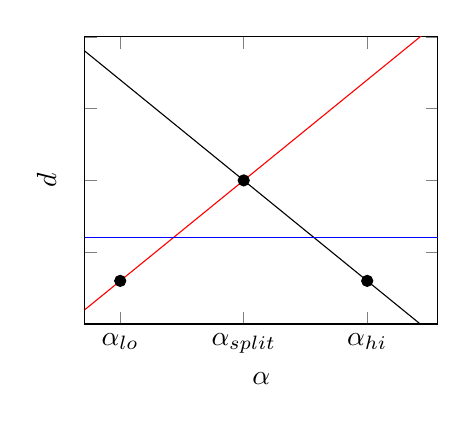
\begin{tikzpicture}
        \begin{axis}[ 
        xlabel=$\alpha$,
        ylabel={$d$},
        xmin=0.4,
        xmax=0.9,
        xtick={0.45,0.625,0.8},
        xticklabels={$\alpha_{lo}$, $\alpha_{split}$, $\alpha_{hi}$},
        width=0.5\textwidth,
        yticklabels={,,}
        ] 
        \addplot[mark=none, red] {-3+8*x}; 
        \addplot[mark=none, black] {-8*x+7};
        \addplot[mark=none, blue] {1.2};
        \addplot [only marks] table {
        0.45   0.6
        0.625  2
        0.8    0.6
        };
        \end{axis} 
    \end{tikzpicture}
    \caption{Simply calculating the split values between the start and the end value of the range $[\alpha_{lo}, \alpha_{hi}]$ will not necessarily lead to the optimal values. By doing so, the blue line (constant $d$ value) will not be considered.}
    \label{fig:notoptimal}
\end{figure}

In order to solve this, we can recursively check each resulting interval again if it contains different merging behaviors.

\begin{figure}[H]
    \centering
    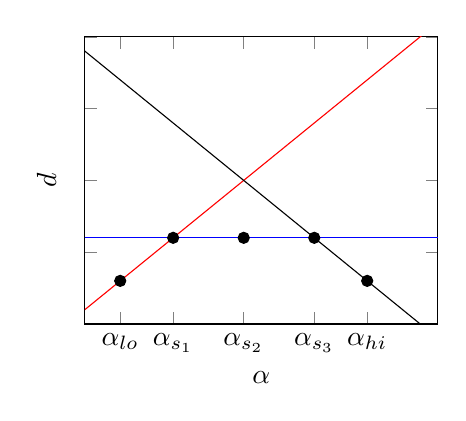
\begin{tikzpicture}
        \begin{axis}[ 
        xlabel=$\alpha$,
        ylabel={$d$},
        xmin=0.4,
        xmax=0.9,
        xtick={0.45,0.525,0.625,0.725,0.8},
        xticklabels={$\alpha_{lo}$, $\alpha_{s_1}$, $\alpha_{s_2}$, $\alpha_{s_3}$, $\alpha_{hi}$},
        width=0.5\textwidth,
        yticklabels={,,}
        ] 
        \addplot[mark=none, red] {-3+8*x}; 
        \addplot[mark=none, black] {-8*x+7};
        \addplot[mark=none, blue] {1.2};
        \addplot [only marks] table {
        0.45   0.6
        0.525  1.2
        0.625  1.2
        0.725  1.2
        0.8    0.6
        };
        \end{axis} 
    \end{tikzpicture}
    \caption{Simply calculating the split values between the start and the end value of the range $[\alpha_{lo}, \alpha_{hi}]$ will not necessarily lead to the optimal values. By doing so, the blue line (constant $d$ value) will not be considered.}
    \label{fig:notoptimal2}
\end{figure}

By calculating the split points recursively, the example in figure \ref{fig:notoptimal2} will result in the intervals $[\alpha_{lo}, \alpha_{s_1}]$, $[\alpha_{s_1}, \alpha_{s_2}]$, $[\alpha_{s_2}, \alpha_{s_3}]$ and $[\alpha_{s_3}, \alpha_{s_{hi}}]$. The optimal distance between $\alpha_{s_1}$ and $\alpha_{s_3}$ is covered now, but the results contain one unncessary interval as $\alpha_{s_2}$ still splits two intervals. The algorithm can check if older splits are still relevant, however the runtime cost to do so will be more expensive than carrying one additional interval with the same distance. We can use this knowledge and adapt algorithm \ref{alg:alphalinkage1}.

\begin{algorithm}[H]
    \KwData{input data $p_1, ..., p_N$, initial states $st$}
    \KwResult{$k$ intervals $[\alpha_0, \alpha_1], ..., [\alpha_{k-1},\alpha_k]$}
    \For{$iteration\gets1$ \KwTo $N-1$}{
        \ForEach{state $s \in st$}{%
        remove state $s$\;
        ranges $\gets$ find ranges between $s.\alpha_{lo}$ and $s.\alpha_{hi}$\;
        \ForEach{range $r \in ranges$}{%
                $cand \gets$ candidate for range\;
                $ms \gets$ merge $cand$\;
                add state $ms$ with range $r$ to the end of $st$\;
        }
      }
    }
    \caption{By calculating the split points between $\alpha_{lo}$ and $\alpha_{hi}$ recursively, we ensure that no optimal interval is left out.}
    \label{alg:alphalinkage2}
\end{algorithm}

As experimental results turn out to need a lot of memory (up to $\approx$ 20 GB for 300 points and 20,000 states), we want to adapt algorithm \ref{alg:alphalinkage2} so that it uses less memory. The memory usage scales relative to the amount of currently in-memory stored states, so the goal is to reduce these. As the amount of states is much larger than the amound of iterations, we calculate and evaluate the leave nodes of the tree and keep the alternative merges stored. This results in algorithm \ref{alg:alphalinkage3}.

\begin{algorithm}[H]
    \KwData{input data $p_1, ..., p_N$, initial states $st$}
    \KwResult{$k$ intervals $[\alpha_0, \alpha_1], ..., [\alpha_{k-1},\alpha_k]$}
    \While{$|st| > 0$}{
        \ForEach{state $s \in st$}{%
        remove state $s$\;
        \eIf{$s$ is final}{
          evaluate $s$\;
          }{
          ranges $\gets$ find ranges between $s.\alpha_{lo}$ and $s.\alpha_{hi}$\;
            \ForEach{range $r \in ranges$}{%
                    $cand \gets$ candidate for range\;
                    $ms \gets$ merge $cand$\;
                    add state $ms$ with range $r$ to the beginning of $st$\;
            }
         }
      }
    }
    \caption{Instead of calculating the nodes layerwise, this algorithm works pathwise, i.e. it goes down one path of a tree to a leaf node and evaluates it before continuing with the next split. This approach needs much less memory than the previous algorithms and has about the same runtime as shown in figure \ref{fig:performance}.}
    \label{alg:alphalinkage3}
\end{algorithm}

\begin{figure}[H]
\centering
\begin{minipage}{.45\textwidth}
  \centering
  \includegraphics[width=\linewidth]{plots/memory_mnist_ac}
\end{minipage}\hfill
\begin{minipage}{.45\textwidth}
  \centering
  \includegraphics[width=\linewidth]{plots/runtime_mnist_ac}
\end{minipage}
\caption{The depth first implementation needs less memory and also has a better runtime compared to the breadth first implementation.}
\label{fig:performance}
\end{figure}

Instead of merging iteratively and steadily shrinking the intervals, we propose an algorithm with a geometric motivation. We are again evaluating an interval $[\alpha_{lo}, \alpha_{hi}]$, but we interprete the different merges as linear functions depending on $\alpha$. We can start by calculating the merge candidate for the start value $\alpha_{lo}$ and calculate the next intersection that will yield to the next merge. By calculating all the intersections of linear functions, we can also determine all the different intervals for the range $[\alpha_{lo}, \alpha_{hi}]$, where different merging behaviors occure. Algorithm \ref{alg:alphalinkage4} describes this procedure.

\begin{algorithm}[H]
    \KwData{input data $p_1, ..., p_N$, start value $\alpha_{lo}$, end value $\alpha_{hi}$}
    \KwResult{$k$ intervals $[\alpha_0, \alpha_1], ..., [\alpha_{k-1},\alpha_k]$}
    $\alpha \gets \alpha_{lo}$\;
    linear function $lf \gets$ get lf for alpha\;
    \While{$\alpha < \alpha_{hi}$}{
        $\alpha_{new} \gets$ calculate next split for $\alpha$\; 
        $lf \gets$ get lf for $\alpha_{new}$\;
        $\alpha \gets \alpha_{new}$
    }
    \caption{}
    \label{alg:alphalinkage4}
\end{algorithm}

\begin{figure}[H]
    \centering
    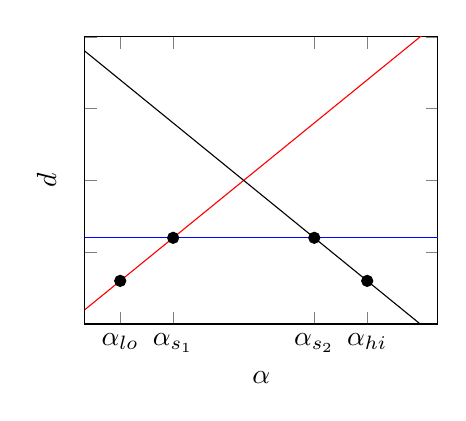
\begin{tikzpicture}
        \begin{axis}[ 
        xlabel=$\alpha$,
        ylabel={$d$},
        xmin=0.4,
        xmax=0.9,
        xtick={0.45,0.525,0.725,0.8},
        xticklabels={$\alpha_{lo}$, $\alpha_{s_1}$, $\alpha_{s_2}$, $\alpha_{hi}$},
        width=0.5\textwidth,
        yticklabels={,,}
        ] 
        \addplot[mark=none, red] {-3+8*x}; 
        \addplot[mark=none, black] {-8*x+7};
        \addplot[mark=none, blue] {1.2};
        \addplot [only marks] table {
        0.45   0.6
        0.525  1.2
        0.725  1.2
        0.8    0.6
        };
        \end{axis} 
    \end{tikzpicture}
    \caption{Simply calculating the split values between the start and the end value of the range $[\alpha_{lo}, \alpha_{hi}]$ will not necessarily lead to the optimal values. By doing so, the blue line (constant $d$ value) will not be considered.}
    \label{fig:optimal}
\end{figure}

\section{Performance Optimizations}

In order to have real-world applications, the proposed algorithms should run in an efficient way, i.e. it should not take the $\alpha$-linkage algorithms too much time to run. A first python implementation took days to run, but switching to C++ and using its advantages took down the runtime to hours. However, there are more optimization methods that we used in order to improve the runtime.

\subsection{Dynamic Programming}

One of the most time-consuming parts was the calculating of the distances. For each pair of clusters $C_i, C,j$ the distance had to be calculated for each clustering state. We optimized this by using dynamic programming and stored the distance matrices $D_{lower}$ and $D_{upper}$ for each state. The naming results from the different interpolation settings where we interpolate from one linkage distance (lower) to another linkage distance (upper), e.g. the setting in equation \ref{eq:singlecomplete} describes the interpolation from single linkage (lower) to complete linkage (upper). In this example we then store the pairwise distances for both single linkage and complete linkage and in order to find the merge candidates we have to do iterate over the distance matrices instead of calculating the distances over and over again. When we merge two clusters, we then update the distance matrices for the given state. Table \ref{dp:distances} shows an example for the pairwise distances of clusters $i$ and $j$.

\begin{table}[H]
    \centering
    \begin{tabular}{|l | l l l l l|}
    \hline
    j\textbackslash i & 0 & 1 & 2 & 3 & 4\\ \hline
    0 & 0 & 1.243 & 1.512 & 2.468 & 5.1243\\
    1 & 1.243 & 0 & 2.443 & 3.1412 & 4.443\\
    2 & 1.512 & 2.443 & 0 & 3.8988 & 6.827\\
    3 & 2.468 & 3.1412 & 3.8988 & 0 & 5.72\\
    4 & 5.1243 & 4.443 & 6.827 & 5.72 & 0\\ \hline
    \end{tabular}
    \caption{Storing the pairwise distances of all clusters avoids calculating the distances over and over again.}
    \label{dp:distances}
\end{table}

One observation that we can make is that the matrix has a lot of redundant values, because $D(i,j) = D(j,i)$. Removing these rendundant values will result in a trade-off between copying and indexing costs and will be discussed in the following section. Another optimization we can do is storing the indices of the active clusters, i.e. the clusters that can get merged. Once two clusters got merged, they cannot be merged any further, only the resulting cluster can. So we then do not have to consider the old clusters anymore and can remove them from the set of active indicies. This allows us to find the merge candidates faster as the pool of candidates gets smaller.

\subsection{Trade-Off between Copying and Indexing Costs}

Currently we can access the costs for a pair of clusters $C_i$ and $C_j$ through $D[i,j]$ or $D[i + j * width]$ for flattened matrices. These indices are very easy to calculate. In order to remove the redundant values from the distance matrix we remove all values below the diagonal as shown in table \ref{dp:distances2}.

\begin{table}[h]
    \centering
    \begin{tabular}{|l | l l l l l|}
    \hline
    j\textbackslash i & 0 & 1 & 2 & 3 & 4\\ \hline
    0 & 0 & 1.243 & 1.512 & 2.468 & 5.1243\\
    1 & \cellcolor{gray!25} & 0 & 2.443 & 3.1412 & 4.443\\
    2 & \cellcolor{gray!25} & \cellcolor{gray!25} & 0 & 3.8988 & 6.827\\
    3 & \cellcolor{gray!25} & \cellcolor{gray!25} & \cellcolor{gray!25} & 0 & 5.72\\
    4 & \cellcolor{gray!25} & \cellcolor{gray!25} & \cellcolor{gray!25} & \cellcolor{gray!25} & 0\\ \hline
    \end{tabular}
    \caption{Storing the pairwise distances of all clusters avoids calculating the distances over and over again.}
    \label{dp:distances2}
\end{table}

In addition to that we can also remove the diagonal values as they represent the distances between the same clusters and are thus always zero. This results in table \ref{dp:distances3}.

\begin{table}[H]
    \centering
    \begin{tabular}{|l | l l l l l|}
    \hline
    j\textbackslash i & 0 & 1 & 2 & 3 & 4\\ \hline
    0 & \cellcolor{gray!25} & 1.243 & 1.512 & 2.468 & 5.1243\\
    1 & \cellcolor{gray!25} & \cellcolor{gray!25} & 2.443 & 3.1412 & 4.443\\
    2 & \cellcolor{gray!25} & \cellcolor{gray!25} & \cellcolor{gray!25} & 3.8988 & 6.827\\
    3 & \cellcolor{gray!25} & \cellcolor{gray!25} & \cellcolor{gray!25} & \cellcolor{gray!25} & 5.72\\
    4 & \cellcolor{gray!25} & \cellcolor{gray!25} & \cellcolor{gray!25} & \cellcolor{gray!25} & \cellcolor{gray!25} \\ \hline
    \end{tabular}
    \caption{Storing the pairwise distances of all clusters avoids calculating the distances over and over again.}
    \label{dp:distances3}
\end{table}

The matrices are now smaller, so they need less memory. In the example, we changed a matrix of the size $25$ to a matrix of the size $10$. In general a matrix of the size $n$x$n$ will be compressed to a matrix of the size $\frac{n^2-n}{2}$. The lower amount of needed memory also results in less copying costs that will lead to a better runtime. However, the indexing is not as easy anymore. For easier storage, we again work with flattened matrices, the indexing for the resulting list is shown in equation \ref{eq:indexing}.

\begin{equation}
    \begin{aligned}
        index(i,j) = \frac{width * (width - 1)}{2} - \frac{(width - j) * (width - j - 1)}{2} + i - j - 1
    \end{aligned}
    \label{eq:indexing}
\end{equation}

Calculating this index in a nested loop is very expensive, however we calculate the part that does not depend on $i$ in the outer loop and thus only need to add $i$ in the inner loop. This does not only yield to a lower memory usage of $\approx 30\%$, but also increases the runtime by TODO.

\todo[inline]{runtime improvement factor}

\subsection{Implementation-specific Optimizations}

In order to optimize the implementation even further, we will have a look into the implementation. One optimization that already was briefly described is the flatterning of the matrices, so the resulting list will be one-dimensional and can be iterated easier and faster.\\

Another observation is that copy operations are computationally expensive, so we avoid them as much as possible. In the described algorithms (\ref{alg:alphalinkage1}, \ref{alg:alphalinkage2} and \ref{alg:alphalinkage3}) we removed a state from the list of states and added other states. In an optimized way, we do not remove the state and just overwrite the state with the resulting state. Once there are splits in the current interval, the state gets overwritten and additional states get added to the list.\\

We can also optimize the way of updating the distance matrices. Instead of adding new clusters there for a merge of clusters $i$ and $j$ we update the distances of $i$ to all active clusters with the distances of the resulting cluster. The distances of the cluster $j$ will not be considered for merges anymore as the index $j$ gets removed from the active indices. This has the advantage that the size of the distance matrices will not increase after merges.\\

Also, the data types make an important contribution to the memory usage. Instead of using double precision floating point values, single precision is enough to clearly identify and separate all the resulting intervals. Same goes for the distances as we only need the minimum and maximum distances, that are not effected by loss of precision. To store the indices of the clusters, we know that they will not exceed $2^{16}$, so they can be store as half precision values.

% \chapter{Optimizing the Metric}
\label{sec:beta}

In a similar fashion as described in section \ref{chapter:alphalinkage}, this sections aims to find an optimized feature representation that is a linear combination of several metrics. For instance, images can have a 2-dimensional pixel representation and a text describing each image. Combining these features for clustering tasks can be problematic as it is not trivial how the optimal weight between these features should be. Does a word describe more than a fragment of the image, are the features equally important or does the pixel image lead to better clusterings? With $\beta$-linkage we provide a framework based on $\alpha$-linkage that calculates different merges based on linear combinations of representations and leads to optimized clusterings.

\begin{figure}[h]
    \centering
    \includegraphics[width=0.7\textwidth]{images/ExampleDataset}
    \caption{Combining several metrics seems often natural and can lead to improved results as in this example where we project a dataset on the $x_1$- and the $x_2$-axis.}
    \label{fig:metrics}
\end{figure}

For instance, figure \ref{fig:metrics} shows a set of points that might be put in clusters easily. However, if you only look at the distance regarding the $x_1$-axis or the $x_2$-axis, a perfect clustering will no longer be possible, because each of the axes does not describe the spatial correlation anymore. This example is selected on purpose to motivate the following experiments where we learn optimal combinations of different metrics.\\ 

To interpolate between $d_0$ and $d_1$, we use the same interpolation as discussed in section \ref{chapter:alphalinkage}. We use a parameter $\beta \in [0,1]$ and weight the metrics as shown below.

\begin{align}
d_\beta(x,x') &= (1 - \beta) \cdot d_0(x,x') + \beta \cdot d_1(x,x') \nonumber \\
&= d_0(x,x') + \beta \cdot (d_1(x,x') - d_0(x,x'))
\label{eq:betalinkage}
\end{align}

We can then compute all possible discontinuities by comparing the distances of given clusters $(x, x')$ and $(y, y')$. As $d_\beta(x,x')$ is a linear function depending on $\beta$ (see equation \ref{eq:betalinkage}), we can compute all discontinuities by solving the following equation.

\begin{equation*}
    \begin{aligned}
      \begin{gathered}
        d_\beta(x,x') = d_\beta(y,y')\\
        (1 - \beta) \cdot d_0(x,x') + \beta \cdot d_1(x,x') = (1 - \beta) \cdot d_0(y,y') + \beta \cdot d_1(y,y')\\
        d_0(x,x') - \beta \cdot d_0(x,x') + \beta \cdot d_1(x,x') = d_0(y,y') - \beta \cdot d_0(y,y') + \beta \cdot d_1(y,y')\\
        \beta \cdot (- d_0(x,x') + d_1(x,x') + d_0(y,y') - d_1(y,y')) = - d_0(x,x') + d_0(y,y')\\
        \beta = \frac{- d_0(x,x') + d_0(y,y')}{- d_0(x,x') + d_1(x,x') + d_0(y,y') - d_1(y,y')}
        \label{eq:discont}
      \end{gathered}
    \end{aligned}
\end{equation*}
As we know that the function $d_\beta$ is a linear function depending on $\beta$ and we showed that all discontinuities depend on four points, we know that there are at most $O(n^4)$ well-defined intervals $\mathcal{I}_i \in [0,1]$ for any clustering instance $S$, i.e. in any interval $\mathcal{I}_i$ the algorithm will merge the same two points. In order to efficiently calculate and evaluate all resulting cluster trees, we use an algorithm similar to algorithm \ref{alg:alphalinkage4}, but adapted to $\beta$-linkage.

\begin{algorithm}
\textbf{Input:} Metrics $\dZero$ and $\dOne$, parameter $\beta \in [0,1]$, and clustering instance $S = \{x_1, \dots, x_n\}$.
\begin{enumerate}[nosep, leftmargin=*]
\item Let $\mathcal{N} = \{\leaf(x_1), \dots, \leaf(x_n)\}$ be the initial set of nodes (one leaf per point).
\item While $|\mathcal{N}| > 1$
\begin{enumerate}[nosep, leftmargin=*]
  \item Let $A, B \in \mathcal{N}$ be the clusters in $\mathcal{N}$ minimizing $\max_{a \in A, b \in B} \dbeta(a, b)$.
  \item Remove nodes $A$ and $B$ from $\mathcal{N}$ and add $\node(A,B)$ to $\mathcal{N}$.
\end{enumerate}
\item Return the cluster tree (the only element of $\mathcal{N}$).
\end{enumerate}
\caption{$\beta$-linkage Clustering}
\label{alg:betalinkage}
\end{algorithm}

A slight adaption that we need is to normalize the features such that for $\beta = 0.5$ we equally weight both distance matrices. We achieve this by dividing the features $f_1, \dots, f_k$ through the maximum value $f_{max}$. In this way, we scale the features into $[0,1]$ and do not lose the proportions as it would happen when e.g.\ using a min-max-scaler.

% % \chapter{$\alpha$-$\beta$-Linkage}

\section{Bilinear Interpolation between three different linkage strategies}

\section{Adapted Algorithm}

% \chapter{Experimental Setup}

This work evaluates the proposed algorithms for image and text data. This chapter describes the used datasets, the evaluation methods and the experimental setups.

\section{Datasets}
\label{sec:datasets}

\subsection{Never Ending Language Learner data}

The Never Ending Language Learner (NELL) is a learning agent that reads the web, extracts data and verfies beliefs \cite{Mitchell:2015:NL:2886521.2886641}\cite{Mitchell:2018:NL:3210350.3191513}. NELL for example knows that "Pittsburgh" is located in "Pennsylvania". These beliefs represent different noun-phrases such as "Pittsburgh" and "Pennsylvania". The noun-phrases belong to certain categories. "Pittsburgh" is a "City" and "Pennsylvania" is a "State". These subcategories both belong to the main category "Geopolitical Location". While there are already different subcategories, the goal for a hierarchical clustering algorithm here is to extract new useful subcategories.

The used dataset, extracted web-information by NELL, contains 32 different main categories, such as "Animal", "Location" or "Person". Each of these consists of up to 250 different entities that belong to different subcategories. Examplary entites for the category "Animal" are "Otter", "Squirrel" or "Wolf". 

This thesis shows in chapter \ref{sec:results} the learned subcategories.

\subsection{MNIST handwritten digits}

The MNIST handwritten digit database contains images of the handwritten digits from zero to nine \cite{lecun-mnisthandwrittendigit-2010}. Samples of these images are shown in figure \ref{fig:mnist} Its training set contains a total of 60,000 images, where each image is represented as a 784-dimensional vector corresponding to a greyscale image with 28x28 pixels.

\begin{figure}[h]
    \centering
    \includegraphics[width=0.7\textwidth]{images/mnist}
    \caption{The MNIST handwritten digits database contains 60,000 greyscale images of handwritten digits ranging from zero to nine. These samples show ten randomly drawn samples for each label represented as a 28x28 pixel image \cite{lecun-mnisthandwrittendigit-2010}.}
    \label{fig:mnist}
\end{figure}

The goal of clustering MNIST images is to find an unsupervised learning method that can distinguish between greyscale images. In addition, we can define various clustering tasks where we pick a subsample of the ten labels and then try to transfer the results to other subsamples. For example, we first cluster images labeled as zero, one, two, three or four and later apply the knowledge the learned gained for clustering images labeled as five, six, seven, eight or nine. Theses types of experiments allow high-level transfer learning if we define several different clustering tasks, e.g. for five different labels there are $10 \choose 5$ $= 252$ different combinations of labels.

Another obsevation that results from hierarchical clustering is the similarity of different labels, i.e. which labels are likely to get clustered together.

\subsection{CIFAR-10}

Another image dataset this thesis uses for evaluation is the CIFAR-10 dataset that contains 60,000 RGB images of ten different categories \cite{Krizhevsky2009LearningML}. Each image consists of 32x32 pixels and is thus represented as a 3072-dimensional vector (32x32x3). The categories and ten random images from each are shown in figure \ref{fig:cifar10}.

\begin{figure}[h]
    \centering
    \includegraphics[width=0.7\textwidth]{images/cifar10}
    \caption{The CIFAR-10  database contains 60,000 RGB images of the ten shown different classes. These samples show ten randomly drawn samples for each label represented as a 32x32 pixel image \cite{Krizhevsky2009LearningML}.}
    \label{fig:cifar10}
\end{figure}

As the amount of images and the amount of classes is equal to the ones in the MNIST database, we can also try similar experiments. The main difference is that the images consist of RGB pixels instead of greyscale values.

\subsection{CIFAR-100}

The CIFAR-100 dataset contains similar images, but instead of 6,000 images each for 10 classes, it consists of 600 images each for 100 classes. The classes are divided into 20 superclasses each containing five subclasses. Examples of superclasses and corresponding subclasses are shown in table \ref{table:cifar100data}. 

\begin{table}[h]
    \centering
    \begin{tabular}{|l|l|}
    \hline
    superclass      & subclasses                                  \\ \hline
    aquatic mammals & beaver, dolphin, otter, seal, whale         \\
    fish            & aquarium fish, flatfish, ray, shark, trout  \\
    flowers         & orchids, poppies, roses, sunflowers, tulips \\
    people          & baby, boy, girl, man, woman                 \\ 
    reptiles        & crocodile, dinosaur, lizard, snake, turtle  \\ \hline               
    \end{tabular}
    \caption{The CIFAR-100 dataset contains 20 different superclasses, each with five different subclasses leading to 100 classes overall. The images are represented in the same way as in the CIFAR-10 dataset, i.e. by a 3072-dimensional vector \cite{Krizhevsky2009LearningML}.}
    \label{table:cifar100data}
\end{table}

Having superclasses and subclasses allows clustering between different subclasses within a superclass and also between different superclasses. This allows more experiments than for the CIFAR10 data.

\section{Cost functions}

In order to evaluate the quality of a clustering, we need some kind of cost function that compares the generated clustering $C_1,...,C_k$ with the target clustering $C_1^*, ..., C_k^*$. One method to compare them is the majority distance as shown in equation \ref{eq:majoritydistance} where $n$ ist the number of sampled points.

\begin{equation}
    \begin{aligned}
        cost_{majority}(C_{1:k}, C_{1:k}^*) = \frac{1}{n} \sum\limits_{i=1}^{k} (\|C_i\| - \max\limits_j \|C_i \cap C_j^*\|)
    \end{aligned}
    \label{eq:majoritydistance}
\end{equation}

Another way to compare two clusterings in by using the hamming distance between the generated and the target clusterings defined as shown in figure \ref{eq:hammingdistance}.

\begin{equation}
    \begin{aligned}
        cost_{hamming}(C_{1:k}, C_{1:k}^*) = 
    \end{aligned}
    \label{eq:hammingdistance}
\end{equation}

However, the hamming distance consists of an assignment problem to find the optimal matching $\sigma$ between the generated clusters and the target clusters. Table \ref{table:matching} shows how such a matching can look like.

\begin{table}[h]
    \centering
    \begin{tabular}{|l | l l l l l|}
    \hline
    j\textbackslash i & 1 & 2 & 3 & 4 & 5\\ \hline
    1 & 20 & \cellcolor{blue!25}15 & 30 & 50 & 40\\
    2 & 80 & 10 & \cellcolor{blue!25}15 & 20 & 30\\
    3 & \cellcolor{blue!25}20 & 30 & 50 & 80 & 60\\
    4 & 30 & 50 & 40 & \cellcolor{blue!25}20 & 10\\
    5 & 20 & 30 & 40 & 50 & \cellcolor{blue!25}25\\ \hline
    \end{tabular}
    \caption{In order to calculate the hamming distance between two clusterings, we have to calculate the optimal mapping that results in lowest distance for these two clusterings. For random distances between clusterings $C_1^i, ..., C_k^i$ and $C_1^j, ..., C_k^j$ we can calculate the optimal mapping (blue highlighted cells) in a brute force way or more efficiently with the hungarian method \cite{kuhn1955hungarian}\cite{munkres1957algorithms}.}
    \label{table:matching}
\end{table}

While solving the assignment with a brute force strategy would result in $O(n!)$ complexity, Harold Kuhn introduced the hungarian method to solve the problem in $O(n^4)$ complexity \cite{kuhn1955hungarian}. Later on, James Munkred modified the algorithm to $O(n^3)$ complexity \cite{munkres1957algorithms}. A detailed explanation of the hungarian method is included in appendix \ref{sec:hungarian}.

\section{Experiments}

In order to find new subclusters for the NELL data, we cluster each of the 32 main categories seperately. This results in 32 different clustering tasks, where we compare the results of each clustering task with the target labels using the majority distance function. We will receive a cost function $cost(\alpha)$, that shows us for which value of $\alpha$ the resulting clusterings are good, for each category. By averaging all cost functions, we know for which values of $\alpha$ the $\alpha$-linkage performs well in general. Beside having a value of $\alpha$ that can be used for other clustering tasks, the experiments also give different representation levels of clusters that are discussed in section \ref{sec:results}.

To cluster the image data, we set up $10 \choose 5$ $= 252$ different experiments by selecting all combinations of five out of the ten labels. In order to do so in efficient time, we subsample the dataset to 60 points for each label, so one experiment will cluster 300 points. By having a fixed set of point, we can show that a certain value of $\alpha$ will lead to good results for the subsampled data. We will use this kind of experiments for all in section \ref{sec:datasets} mentioned image datasets where all RGB-channels are treated equally for colored images.

In addition to these experiments, we will try to cluster as diverse as possible superclasses of the CIFAR100 dataset by manually picking the five superclasses fish, flowers, household furniture, people and vehicles 1. For each superclass we pick one subclass and evaluate the results for all $5 *$ $5 \choose 1$ $= 25$ different combinations of subclasses. In addition to the experiments with $k = 5$ clusters, we compare these results to the results for picking two different subclasses of each superclass ($5 *$ $5 \choose 2$ $= 50$ different experiments) resulting in $k = 10$ clusters and also for picking three different subclasses ($5 *$ $5 \choose 3$ $= 50$ different experiments) resulting in $k = 15$ clusters.

In comparison to picking as diverse as possible superclasses, we also evaluate the performance for as similar as possible subclasses. Similar subclasses are already given in the dataset through the subclasses within one superclass. We then evaluate the majority and the hamming cost for each superclass and again average the cost over all 20 superclasses to evaluate an optimal value for the parameter $\alpha$.

The results of these experiments are discussed in the following section \ref{sec:results}. % Experimental Setup

% \chapter{Experimental Results and Discussion}
\label{sec:results}

\todo[inline]{Update plots.}
\todo[inline]{More results.}

We evaluated the in chapter \ref{chapter:alphalinkage} proposed algorithms with the in chapter \ref{chapter:datasets} discussed datasets aiming to find new subcategories for the text data and to generate better clusterings overall. The quality of the clusterings was calculated with the in chapter \ref{chapter:costfunctions} explained cost functions.

\section{Algorithm Selection}

In general we evaluate two different types of experiments that apply for most of the datasets. Only for the synthetic dataset, we evaluate the data distribution shown in figure \ref{fig:disksrings}.

\paragraph{Batch Data Experiments.} In the first one, we evaluate certain data batches, i.e. we subsample the $n$-th set of points in sorted order for each of the target classes. To generalize the experiments for larger datasets, we average over multiple batches. In our experiments, we evaluate all distinct combinations of $k$ classes, e.g. for multiple datasets we have 10 target classes and use 5 labels for our experiments, i.e. we evaluate all $10 \choose 5$ combinations to cover all possible label subsets.

\paragraph{Randomized Experiments.} In the other setting, we follow \cite{NIPS2016_6385} and \cite{pmlr-v70-finn17a}. We select the points for certain classes by random. Averaging over a large number of clustering instances allows us to cover a major fraction of the dataset. To clusters a subset of the target classes, we also select the classes by random. Overall, in case both experimental settings agree, we know that the results are generalized well for the underlying data distribution.

\paragraph{Synthetic Experiments.} Here we generated 1000 clustering instances by random given the data distribution shown in section \ref{chapter:datasets}, i.e. all instances contain four classes, two rings and two disks. In figure \ref{fig:syntheticexperiments} we observe that all three linkage strategies perform very similarly. Only single linkage does slightly better with an error below $25\%$ while both average and complete linkage are above $25\%$. Interpolating between single and linkage (a) leads to significantly lower errors, where interpolating between average and complete linkage (b) does not lead to improvements. As this example motivates interpolating between single and complete linkage, we elaborate this setting further.

\begin{figure}[H]
\centering
\begin{minipage}{.45\textwidth}
  \centering
  \subcaptionbox{SC.}
  {\includegraphics[width=\linewidth]{plots/ringsanddiskssc}}
\end{minipage}\quad
\begin{minipage}{.45\textwidth}
  \centering
  \subcaptionbox{AC.}
  {\includegraphics[width=\linewidth]{plots/ringsanddisksac}}
\end{minipage}
\caption{%
  %
  }
  %
\label{fig:syntheticexperiments}
\end{figure}

\paragraph{NELL Experiments.} In order to find new subclusters for the NELL data, we cluster each of the 32 main categories seperately. This results in 32 different clustering tasks, where we compare the results of each clustering task with the target labels using the majority distance function. We will receive a cost function $cost(\alpha)$, that shows us for which value of $\alpha$ the resulting clusterings are good, for each category. By averaging all cost functions, we know for which values of $\alpha$ the $\alpha$-linkage performs well in general. Beside having a value of $\alpha$ that can be used for other clustering tasks, the experiments also give different representation levels of clusters that are discussed in section. First, we started evaluating all tasks with a maximum of 250 points per task. Figure \ref{fig:nellresults} shows the result for all three different interpolation strategies.

\begin{figure}[h]
\centering
\begin{minipage}{.3\textwidth}
  \centering
  \includegraphics[width=\linewidth]{plots/nell_sc}
\end{minipage}
\begin{minipage}{.3\textwidth}
  \centering
  \includegraphics[width=\linewidth]{plots/nell_sa}
\end{minipage}
\begin{minipage}{.3\textwidth}
  \centering
  \includegraphics[width=\linewidth]{plots/nell_ac}
\end{minipage}
\caption{$\alpha$-linkage using 250 points for each clustering instance gives minor improvements for the NELL data when clustering between single and complete (left) and average and complete linkage (right). As complete linkage performs best of our input strategies, interpolating between single and average linkage (middle) does not lead to improvements.}
\label{fig:nellresults}
\end{figure}

We see minor improvements when clustering between single and complete and average and complete linkage. On the other hand, interpolating between single and average linkage did not lead to any improvement. In order to evaluate the results further, we have a closer look at the curves and see that the overall improvement we get is $0.53\%$, a reduction from $15.9725\%$ (complete linkage) to $15.4422\%$ ($\alpha_{SC}(0.826)$) as shown in table \ref{table:nellresults}. An interesting observation is that while single linkage performs very poor overall, interpolating between single and complete linkage gives a better improvement than interpolating between average and complete linkage. To evaluate these experiments we are using the Majority Distance, as for such a large number of target clusters calculating the Hamming distance is not efficient. 

\begin{table}[h]
    \centering
    \begin{tabular}{|l | l|}
    \hline
    Strategy & Majority Cost\\ \hline
    Single Linkage & 0.36871\\
    Average Linkage & 0.248913\\
    Complete Linkage & 0.159725\\
    \cellcolor{green!50}$\alpha_{SC}(0.826)$ & \cellcolor{green!50}0.154422\\
    $\alpha_{AC}(0.826)$ & 0.155697\\\hline
    \end{tabular}
    \caption{Our proposed algorithm reduces the NELL cost by $\Delta cost = 0.53\%$ when using a maximum of 250 points for each class.}
    \label{table:nellresults}
\end{table}

As the algorithm became a lot more efficient during this work, we scaled up the algorithms to use 1,000 instead of 250 points per class. Figure \ref{fig:nellresults1000} shows that in general the error is slightly higher. This is because our experiments contain more different classes. Overall, we again see slight improvements that are shown in table \ref{table:nell1000}. Compared to the previous experiments, the improvements were a bit bigger ($1.2078\%$ leading to an error of $16.6742\%$), however the overall curves look very similar. In this setting, we also evaluated the parameter advising for the first 10 parameters $\alpha^*$ (see figure \ref{fig:nell1000top10}).

\begin{figure}[h]
\centering
\begin{minipage}{.45\textwidth}
  \centering
  \includegraphics[width=\linewidth]{plots/nell_sc_1000}
\end{minipage}
\begin{minipage}{.45\textwidth}
  \centering
  \includegraphics[width=\linewidth]{plots/nell_ac_1000}
\end{minipage}
\caption{$\alpha$-linkage using 1000 points for each clustering instance gives minor improvements for the NELL data when clustering between single and complete (left) and average and complete linkage (right).}
\label{fig:nellresults1000}
\end{figure}

\begin{table}[h]
    \centering
    \begin{tabular}{|l | l|}
    \hline
    Strategy & Majority Cost\\ \hline
    Single Linkage & 0.36871\\
    Average Linkage & 0.291202\\
    Complete Linkage & 0.17882\\
    \cellcolor{green!50}$\alpha_{SC}(0.918)$ & \cellcolor{green!50}0.166742\\
    $\alpha_{AC}(0.855)$ & 0.171083\\\hline
    \end{tabular}
    \caption{Our proposed algorithm reduces the NELL cost by $\Delta cost = 1.2078\%$ when using a maximum of 1000 points for each class.}
    \label{table:nell1000}
\end{table}

\begin{figure}[H]
\centering
\begin{minipage}{.45\textwidth}
  \centering
  \includegraphics[width=\linewidth]{plots/nell_sc_1000_top10}
\end{minipage}
\begin{minipage}{.45\textwidth}
  \centering
  \includegraphics[width=\linewidth]{plots/nell_ac_1000_top10}
\end{minipage}
\caption{$\alpha$-linkage using 1000 points for each clustering instance gives minor improvements for the NELL data when clustering between single and complete (left) and average and complete linkage (right).}
\label{fig:nell1000top10}
\end{figure}

Also, we evaluated the corresponding clusters. As $\alpha$-linkage uses agglomerative hierarchical clustering, we can extract clusters at different levels starting with each noun phrase as its own cluster. Tables \ref{tbl:rooms}, \ref{tbl:clothing} and \ref{tbl:kitchenitems} show some examples for discovered categories.

\begin{table}[H]
  \makebox[\textwidth][c]{
  \small
  \begin{tabular}{cccc}
    \hline\hline
    \textbf{Luxury Room} & \textbf{Bathroom} & \textbf{Guest Room} & \textbf{Suite} \\ \hline
    spacious living room & large ensuite bathroom & elegant rooms & luxurious suites\\
    comfortable living room & spacious marble bathroom & three guest rooms & one bedroom suites\\
    guest room & one bathroom & large guest rooms & spacious suites\\
    lounge room & full bathroom & deluxe guest rooms & deluxe suites\\
    living room & upstairs bathroom & guests rooms & guest suites\\
    superior room & large bathroom & spacious air conditioned rooms & bedroom suites\\
    sleeping room & ensuite bathroom & furnished guest rooms & whirlpool suites\\
    main bedroom & elegant bathroom & comfortable guest rooms & three suites\\
    \hline
  \end{tabular}
  }
  \caption{Proposed Subcategories for ``Office Building Room''.}
  \label{tbl:rooms}
\end{table}

\begin{table}[H]
  \makebox[\textwidth][c]{
  \small
  \begin{tabular}{ccccc}
    \hline\hline
    \textbf{Shoes} & \textbf{Uniform/Costume} & \textbf{Pants} & \textbf{Casual} & \textbf{Specialized} \\ \hline
    shoes & costume & kneepants & stocking cap & long stockings\\
    high heel shoes & work uniforms & baggy pants & workout clothes & wide brimmed hat\\
    sensible shoes & outfits & loose fitting pants & casual clothes & casual wear\\
    old shoes & period costume & slacks & baseball caps & black stockings\\
    pointe shoes & folk costumes & black shorts & skull caps & wear socks\\
    dark shoes & halter top & special clothing & ball caps & high heels\\
    spira shoes & period costumes & white shorts & evening clothes & surf wear\\
    mens shoes & costumes & underpants & ball cap & wear gloves\\
    \hline
  \end{tabular}
  }
  \caption{Proposed Subcategories for ``Clothing''.}
  \label{tbl:clothing}
\end{table}

\begin{table}[H]
  \makebox[\textwidth][c]{
  \small
  \begin{tabular}{cccc}
    \hline\hline
    \textbf{Stove/Oven} & \textbf{Machines} & \textbf{Bowls} & \textbf{Baking Sheets} \\ \hline
    full size stove & cookie cutters & large mixing bowl & oiled baking sheet\\
    full size cooker & automatic washing machine & large serving bowl & rimmed baking sheet\\
    red hot stove & washing machine & small bowl & large baking sheet\\
    plastic jug & bread machine & single bowl & small baking sheet\\
    toaster & cookie cutter & separate bowl & prepared baking sheet\\
    greased baking dish & coffee machine & shallow bowl & ungreased baking sheet\\
    wood burning pizza oven & cooking spray & separate mixing bowl & hot plate\\
    ceramic top stove & coffee grinder & large bowl & greased baking sheet\\
    \hline
  \end{tabular}
  }
  \caption{Proposed Subcategories for ``Kitchen Item''.}
  \label{tbl:kitchenitems}
\end{table}

In addition to using the original features, we also use the word embeddings and the bag-of-contexts representations to evaluate these experiments.

\todo[inline]{Add experiments for new features.}

\paragraph{MNIST Experiments.} For the MNIST images, we evaluate both describes experimental settings with combinations of five out of the ten target classes. In addition to using the raw pixel features. To cluster the data, we set up $10 \choose 5$ $= 252$ different experiments by selecting all combinations of five out of the ten labels. In order to do so in efficient time, we subsample the dataset to 200 points for each label, so one experiment will cluster 1000 points. First, we evaluated the results for both average to complete and single to complete linkage for several batches. Note that we do not discuss the interpolation between single to average linkage in this and the following paragraphs, as experiments did not lead to improvements. First, we show the experiments for the six first batches $b_i, i \in \{0, 1, 2, 3, 4, 5\}$ for interpolating between single and complete linkage.

\begin{figure}[h]
\centering
\begin{minipage}{.3\textwidth}
  \centering
  \includegraphics[width=\linewidth]{plots/mnist-sc-0}
\end{minipage}
\begin{minipage}{.3\textwidth}
  \centering
  \includegraphics[width=\linewidth]{plots/mnist-sc-1}
\end{minipage}
\begin{minipage}{.3\textwidth}
  \centering
  \includegraphics[width=\linewidth]{plots/mnist-sc-2}
\end{minipage}
\begin{minipage}{.3\textwidth}
  \centering
  \includegraphics[width=\linewidth]{plots/mnist-sc-3}
\end{minipage}
\begin{minipage}{.3\textwidth}
  \centering
  \includegraphics[width=\linewidth]{plots/mnist-sc-4}
\end{minipage}
\begin{minipage}{.3\textwidth}
  \centering
  \includegraphics[width=\linewidth]{plots/mnist-sc-5}
\end{minipage}
\caption{Over the first six batches of the MNIST data, interpolating between single and complete linkage shows a similar behavior.}
\label{fig:mnistscbatches}
\end{figure}

As shown in figure \ref{fig:mnistscbatches}, the clustering over the first six batches leads to very similar curves with slightly different errors. Table \ref{table:mnistscbatches} evaluates the results in more detail.

\begin{table}[H]
    \centering
    \begin{tabular}{|l | l l l l l l |}
    \hline
    Strategy & Batch 0 & Batch 1 & Batch 2 & Batch 3 & Batch 4 & Batch 5\\ \hline
    Single Linkage & 0.796901 & 0.797345 & 0.797171 & 0.797405 & 0.796766 & 0.797024\\
    Complete Linkage & 0.490468 & 0.461063 & 0.479825 & 0.475329 & 0.463321 & 0.487111\\
    $\alpha_{opt}$ & 0.87228 & 0.84419 & 0.778498 & 0.83199 & 0.82338 & 0.852251\\
    $cost_{opt}$ & 0.450012 & 0.416433 & 0.431143 & 0.423786 & 0.421103 & 0.446032\\
    $\Delta cost$ & 4.0456\% & 4.463\% & 4.8682\% & 5.1543\% & 4.2218\% & 4.1079\%\\\hline
    \end{tabular}
    \caption{$\alpha$-linkage reduces the cost of the MNIST dataset by up to $\Delta_{max} cost = 5.1543\%$ when interpolating between single and complete linkage.}
    \label{table:mnistscbatches}
\end{table}

Table \ref{table:mnistscbatches} leads to several observations. Clustering points of five classes with a random guess will result in an error of $80\%$. As for all batches single linkage results in an error between $79\%$ and $80\%$, we note that single linkage performs similar than a random guess would. Thus, single linkage is not suitable for the MNIST data. In comparison, complete linkage results in errors below $50\%$ on just using the pixel data. It is not necessarily a great result, but it indicates that grouping high-dimensional pixel features with unsupervised learning can work. Also, we note that the parameter $\alpha_{opt}$ doesn't vary that much and also we notice in figure \ref{fig:mnistscbatches} that for $\alpha \in [0.75,1.0)$ we outperform complete linkage in all cases. As the results are very similar for the used batches, we also average over the batches in figure \ref{fig:mnistscbatchesavg}.

\begin{figure}[H]
    \centering
    \includegraphics[width=0.5\textwidth]{plots/mnist-sc-averaged.png}
    \caption{Evaluating the first six batches of the MNIST data interpolating between single and complete linkage results in major improvements over both single and complete linkage.}
    \label{fig:mnistscbatchesavg}
\end{figure}

\begin{table}[H]
    \centering
    \begin{tabular}{|l | l |}
    \hline
    Strategy & Hamming Cost\\ \hline
    Single Linkage & 0.797102\\
    Complete Linkage & 0.476186\\
    $\alpha_{opt}$ & 0.857\\
    $cost_{opt}$ & 0.439207\\
    $\Delta cost$ & 3.6979\%\\\hline
    \end{tabular}
    \caption{Over the first 12,000 points of the MNIST dataset interpolating between single and complete linkage improves hamming cost by $3.7\%$ }
    \label{table:mnist1000avgsc}
\end{table}

Figure \ref{fig:mnistscbatchesavg} and table \ref{table:mnist1000avgsc} show that by applying $\alpha$-linkage interpolating between single and complete linkage we improve the hamming cost by $3.7\%$ over the first six data batches, i.e. the first 12,000 points of the dataset. Next, we evaluate the randomized experiments for the same interpolation method, where we average over 512 experiments that are run with random label subsets and randomly selected points for each of the selected labels. Figure \ref{fig:mnistscrandom} shows that in this setting we obtain a very similar curve as in the other setting (figure \ref{fig:mnistscbatchesavg}).

\begin{figure}[H]
    \centering
    \includegraphics[width=0.5\textwidth]{plots/mnist-sc-random.png}
    \caption{Selecting labels and points randomly leads to a similar curve when interpolating between single and complete linkage using the MNIST data.}
    \label{fig:mnistscrandom}
\end{figure}

\begin{table}[H]
    \centering
    \begin{tabular}{|l | l | l |}
    \hline
    Strategy & Hamming Cost (Batch) & Hamming Cost (Random)\\ \hline
    Single Linkage & 0.797102 & 0.797215\\
    Complete Linkage & 0.476186 & 0.476355\\
    $\alpha_{opt}$ & 0.857 & 0.857\\
    $cost_{opt}$ & 0.439207 & 0.440932\\
    $\Delta cost$ & 3.6979\% & 3.5423\%\\\hline
    \end{tabular}
    \caption{Evaluating the randomized setting leads to exactly the same parameter $\alpha_{opt}$ and a similar cost improvement as in the batch setting for the MNIST data.}
    \label{table:mnist1000randomsc}
\end{table}

Table \ref{table:mnist1000randomsc} compares the results for both settings when interpolating between single and complete linkage. We obtain very similar results for single and complete linkage. Also, the optimal parameter $\alpha_{opt}$ is the same in both settings leading to similar improvements in the hamming cost. This means that $\alpha$-linkage is robust over the entire MNIST distribution and with an improvement of more than $3\%$ towards complete linkage it outperforms both used linkage strategies by a major difference. In addition, we also evaluate the greedy parameter advising for the previous experiments.\\

\begin{figure}[H]
\centering
\begin{minipage}{.45\textwidth}
  \centering
  \includegraphics[width=\linewidth]{plots/mnist-sc-top-10}
\end{minipage}
\begin{minipage}{.45\textwidth}
  \centering
  \includegraphics[width=\linewidth]{plots/mnist-sc-random-top-10}
\end{minipage}
\caption{}
\label{fig:mnistsctop10}
\end{figure}

Figure \ref{fig:mnistsctop10} shows that we again obtain very similar results for the batch setting (left) and the random setting (right). By using $k = 3$ parameters $\alpha^*$ the cost drops more than $5\%$ in addition to less than $38\%$. In comparison to the best linkage strategy, i.e. complete linkage, this is an improvement of $\approx 10\%$.\\

Similar to that, we also interpolate between average and complete linkage and evaluate both the batch and the random setting. Figure \ref{fig:mnist1000acbatch} and table \ref{table:mnist1000acbatch} show that the results of the different batches vary much. On the one hand, the parameters $\alpha_{opt}$ have a wider range ($\alpha_{opt} \in [0.53,0.81]$), but on the other hand, we get slightly larger improvements for the hamming cost in comparison to complete linkage.

\begin{figure}[H]
\centering
\begin{minipage}{.3\textwidth}
  \centering
  \includegraphics[width=\linewidth]{plots/mnist-ac-0}
\end{minipage}
\begin{minipage}{.3\textwidth}
  \centering
  \includegraphics[width=\linewidth]{plots/mnist-ac-1}
\end{minipage}
\begin{minipage}{.3\textwidth}
  \centering
  \includegraphics[width=\linewidth]{plots/mnist-ac-2}
\end{minipage}
\begin{minipage}{.3\textwidth}
  \centering
  \includegraphics[width=\linewidth]{plots/mnist-ac-3}
\end{minipage}
\begin{minipage}{.3\textwidth}
  \centering
  \includegraphics[width=\linewidth]{plots/mnist-ac-4}
\end{minipage}
\begin{minipage}{.3\textwidth}
  \centering
  \includegraphics[width=\linewidth]{plots/mnist-ac-5}
\end{minipage}
\caption{Over the first six batches of the MNIST data, interpolating between average and complete linkage shows quite different curves.}
\label{fig:mnist1000acbatch}
\end{figure}

\begin{table}[h]
    \centering
    \begin{tabular}{|l | l l l l l l |}
    \hline
    Strategy & Batch 0 & Batch 1 & Batch 2 & Batch 3 & Batch 4 & Batch 5\\ \hline
    Average Linkage & 0.664952 & 0.672583 & 0.623325 & 0.679929 & 0.657857 & 0.652774\\
    Complete Linkage & 0.490468 & 0.461063 & 0.479825 & 0.475329 & 0.463321 & 0.487111\\
    $\alpha_{opt}$ & 0.7869 & 0.7124 & 0.634 & 0.807697 & 0.536073 & 0.5305\\
    $cost_{opt}$ & 0.458167 & 0.406563 & 0.440964 & 0.451063 & 0.429849 & 0.431631\\
    $\Delta cost$ & 3.2301\% & 5.45\% & 3.8861\% & 2.4266\% & 3.3472\% & 5.548\%\\\hline
    \end{tabular}
    \caption{$\alpha$-linkage reduces the cost of the MNIST dataset by up to $\Delta_{max} cost = 5.548\%$ when interpolating between average and complete linkage.}
    \label{table:mnist1000acbatch}
\end{table}

\begin{figure}[h]
\centering
\begin{minipage}{.45\textwidth}
  \centering
  \includegraphics[width=\linewidth]{plots/mnist-ac-averaged}
\end{minipage}
\begin{minipage}{.45\textwidth}
  \centering
  \includegraphics[width=\linewidth]{plots/mnist-ac-random}
\end{minipage}
\caption{Comparing the batch and the random experients for the MNIST data when interpolating between average and complete linkage leads to similar curves.}
\label{fig:mnistacavg}
\end{figure}

Figure \ref{fig:mnistacavg} shows the comparison between the batch (left) and the random experiments (right). In general, we obtain similarly looking curves, but elaborate the results further in table \ref{table:mnistacavg}.

\begin{table}[h]
    \centering
    \begin{tabular}{|l | l | l |}
    \hline
    Strategy & Hamming Cost (Batch) & Hamming Cost (Random)\\ \hline
    Average Linkage & 0.65857 & 0.679936\\
    Complete Linkage & 0.476187 & 0.476328\\
    $\alpha_{opt}$ & 0.633 & 0.656\\
    $cost_{opt}$ & 0.44314 & 0.439632\\
    $\Delta cost$ & 3.3047\% & 3.6696\%\\\hline
    \end{tabular}
    \caption{}
    \label{table:mnistacavg}
\end{table}

\begin{figure}[H]
\centering
\begin{minipage}{.45\textwidth}
  \centering
  \includegraphics[width=\linewidth]{plots/mnist-ac-top-10}
\end{minipage}
\begin{minipage}{.45\textwidth}
  \centering
  \includegraphics[width=\linewidth]{plots/mnist-ac-random-top-10}
\end{minipage}
\caption{}
\label{fig:mnistactop10}
\end{figure}

Summarizing, we also obtained very positive results for $d_{AC}$, however the results were not as stable as for $d_{SC}$. In our experiments, we notice that $d_{SC}$ results in more discontinuities (factor $\approx 3$) than $d_{AC}$. This may be because the distance $d(\alpha)$ is wider spread for $d_{SC}$, i.e. $|d_{SC}(\alpha = 1) - d_{SC}(\alpha = 0)| > |d_{AC}(\alpha = 1) - d_{AC}(\alpha = 0)|$. However $d_{AC}$ is dependant on more points, so it may be an indicator for this observation, but not a proof. Figure \ref{fig:mnistactop10} also shows that parameter advising is using with a small value $k$ already and reduces the costs for $k = 3$ by $\approx 5\%$ in addition.

\paragraph{Learning MNIST features.} Differently to just using the raw pixel features, we here apply preprocessing techniques with the intention to generate more accurate clusterings. As in section \ref{sec:imagefeatures} described, we use a Convolutional Neural Network to learn a more robust and lower-dimensional feature representation. Therefore, we use the in appendix \ref{sec:cnnarchitecture} described architecture, train the network with all data and then extract the features by cutting off the last three layers of the network. This then results in a learned 128-dimensional representation for each image.

\begin{figure}[h]
\centering
\begin{minipage}{.45\textwidth}
  \centering
  \subcaptionbox{By evaluating all 252 combinations of five different labels, the average error goes down to $2.6\%$ that makes an improvement of $7.4\%$ compared to complete linkage.}
  {\includegraphics[width=\linewidth]{plots/mnist-cnn-avg}}
\end{minipage}\quad
\begin{minipage}{.45\textwidth}
  \centering
  \subcaptionbox{Evaluating 512 random sets of labels and points gives an eror of $7.1\%$ that is an improvement of $1.9\%$ compared to complete linkage.}
  {\includegraphics[width=\linewidth]{plots/mnist-cnn-random}}
\end{minipage}
\begin{minipage}{.45\textwidth}
  \centering
  \subcaptionbox{Considerung more than one optimal value to evaluate the experiments results in lower costs, e.g. using two values $\alpha_{opt}$ cuts the cost by $50\%$ and using three values results in a cost below $1\%$.}
  {\includegraphics[width=\linewidth]{plots/mnist-cnn-sc-top-10}}
\end{minipage}\quad
\begin{minipage}{.45\textwidth}
  \centering
  \subcaptionbox{On random sets of labels and randomly selected points, taking more than one optimal value $\alpha_{opt}$ also gives major improvements. With three values the cost goes down below $3\%$ that is less than a half of the original optimum.}
  {\includegraphics[width=\linewidth]{plots/mnist-cnn-sc-random-top-10}}
\end{minipage}
\caption{By learning feature representations with a Convolutional Neural Network, we can reduce the overall error a lot compared to clustering raw pixel images.}
\label{fig:mnist1000cnn}
\end{figure}

Figure \ref{fig:mnist1000cnn} shows that single linkage still performs poorly, however the error for both complete linkage and the interval in between are much lower. Also, we note that the improvement using $\alpha$-linkage is large over both settings. However, a Convolutional Neural Network aims at recognizing the characters, so training on all images might be the sole cause of our improvements. Thus, it is more relevant for our experiments to either train the network on a subset of the data or to train the network on a different task in order to transfer the knowledge to unseen data or to a different task.

\paragraph{Learning Subsets of the MNIST Data.} As our goal is also to cluster unseen data, we evaluated another setup, where a CNN was trained on a subset of the dataset. In a first attempt, we trained it on the labels $\{0,1,2,3,4\}$ that are represented with 30,000 of the 60,000 points in the dataset. Figure \ref{fig:mnist1000cnnsub} shows that clustering unseen points (i.e. the CNN did not use these points for training) still results in a lower error than using the raw pixel features where combining seen and unseen points leads to results that are comparable to clusterings with features extracted from a neural network that was trained with all digits. In average, complete linkage resulted in an error of $22.1\%$. The cost for $\alpha_{opt} = 0.67$ is $20.7\%$ and makes an improvement of $1.4\%$. Interesting especially in this setting are the different results of seen and unseen data. In machine learning, the task of applying knowledge to unseen data is commonly known as zero-shot learning. While the error was $0.2\%$ for large parts of the seen data (i.e. clustering the digits $\{0,1,2,3,4\}$), the optimal cost for the unseen data (i.e. clustering the digits $\{5,6,7,8,9\}$) was $24.7\%$ for $\alpha_{opt} = 0.76$. \todo[inline]{plot and discuss randomized experiments}

\begin{figure}[H]
\centering
\begin{minipage}{.3\textwidth}
  \centering
  \subcaptionbox{The learned characters (i.e. labels $\{0,1,2,3,4\}$) can be clustered very well. Similar to training on all labels, the error goes down close to $0\%$.}
  {\includegraphics[width=\linewidth]{plots/mnist-cnn-sub-01234}}
\end{minipage}\quad
\begin{minipage}{.3\textwidth}
  \centering
  \subcaptionbox{Combining three trained ($0,2,4$) with two untrained digits ($6,8$) still leads to an optimal error of $2.1\%$ that is $10\%$ below complete linkage.}
  {\includegraphics[width=\linewidth]{plots/mnist-cnn-sub-02468}}
\end{minipage}\quad
\begin{minipage}{.3\textwidth}
  \centering
  \subcaptionbox{Clustering three untrained ($5,7,9$) with two trained digits ($1,3$) already leads to larger errors of $15.1\%$.}
  {\includegraphics[width=\linewidth]{plots/mnist-cnn-sub-13579}}
\end{minipage}
\begin{minipage}{.3\textwidth}
  \centering
  \subcaptionbox{Even by clustering only untrained characters, the error goes down to $37\%$ that is a major improvement compared to clustering the raw pixel features that resulted in an optimal cost of $44\%$.}
  {\includegraphics[width=\linewidth]{plots/mnist-cnn-sub-56789}}
\end{minipage}\quad
\begin{minipage}{.3\textwidth}
  \centering
  \subcaptionbox{Averaged over all 252 instances, the error for $\alpha_{opt} = 0.67$ is $20.7\%$ and an improvement of $1.4\%$ compared to complete linkage and $23\%$ compared to the raw pixel features.}
  {\includegraphics[width=\linewidth]{plots/mnist-cnn-sub-sc}}
\end{minipage}\quad
\begin{minipage}{.3\textwidth}
  \centering
  \subcaptionbox{Parameter advising results in major improvements for this setting. Using three values $\alpha^* \in \{0.86, 0.67, 0.99\}$ reduces the error by additional $5.3\%$ to $15.5\%$.} 
  {\includegraphics[width=\linewidth]{plots/mnist-cnn-sub-sc-top10}}
\end{minipage}
\caption{Learning features depending on a subset of the represented digits leads to different results. While applying the learned digits still leads to almost perfect clusterings, clustering the unlearned digits leads to worse results that still are much better than applying the raw pixel features.}
\label{fig:mnist1000cnnsub}
\end{figure}

\paragraph{Learning Even and Odd Numbers.} Beside training a neural network on recognizing all digits separately, another learning task to generate feature representations that we used is to learn if an image shows an even or an odd digit. In this setting, we trained the CNN on all images and extracted the feature vectors from the sixth layer. The used network had the same architecture as the one used in the earlier experiments with the only difference of two neurons in the output layer. Figure \ref{fig:mnist_cnn_even_odd} shows that with features trained on a different learning task we still can improve the overall clustering. Complete linkage resulted in a cost of $28.1\%$ for the first data batch, where the optimal alpha $\alpha_{opt} = 0.74$ led to $23.6\%$, an improvement of 4.5\%. The results are only slidely worse than the ones of a network trained to distinguish the digits $\{0,1,2,3,4\}$. Parameter adivising lowers the cost another $5.2\%$ for $n = 3$ values $\alpha^* \in \{0.74, 0.65, 0.76\}$. \todo[inline]{randomized experiments}

\begin{figure}[H]
\centering
\begin{minipage}{.45\textwidth}
  \centering
  \subcaptionbox{Compared to complete linkage, we got an improvement of $4.5\%$ for $\alpha_{opt} = 0.74$.}
  {\includegraphics[width=\linewidth]{plots/mnist-cnn-even-odd-sc}}
\end{minipage}\quad
\begin{minipage}{.45\textwidth}
  \centering
  \subcaptionbox{Applying parameter advising shows significant improvements for small numbers of $k$.}
  {\includegraphics[width=\linewidth]{plots/mnist-cnn-even-odd-sc-top10}}
\end{minipage}
\caption{%
  %
  Clustering features extracted from a CNN that learned to distinguish even from odd numbers with all data led to an optimal cost of $23.6\%$ (a). Parameter advising allows us to minimize the cost ether further to $18.4\%$ for the values $\alpha^* \in \{0.74, 0.65, 0.76\}$ (b).}
  %
\label{fig:mnist_cnn_even_odd}
\end{figure}

\paragraph{Summarized MNIST Results.} Different experimental setups were discussed in this section. First, raw pixel features were used for clustering. Later on, features extracted from Convolutional Neural Networks were used. There, we trained a network on all digits and extracted the feature vectors from the 6th layer of the network that represents each image encoded in a 128-dimensional vector. We used the same representation coming from a network trained on a subset of the images. In addition, we extracted feature vectors from the 9216-dimensional 5th layer of the network that was trained on a subset of the characters. Figure \ref{fig:mnist_overview} gives an overview about the results of the different settings for both the 252 experiments evaluating all different combinations of five labels within the first data batch as well as the randomized experiments where we evaluated 512 experiments with radomized digits and points from the entire data. \todo{add table}

\begin{figure}[H]
\centering
\begin{minipage}{.45\textwidth}
  \centering
  \subcaptionbox{Evaluating the experiments of all combinations of five labels within the first batch shows strong discontinuities.}
  {\includegraphics[width=\linewidth]{plots/mnist_overview}}
\end{minipage}\quad
\begin{minipage}{.45\textwidth}
  \centering
  \subcaptionbox{Evaluating 512 experiments with randomized digits and points shows similar results with smoother curves.}
  {\includegraphics[width=\linewidth]{plots/mnist_overview_random}}
\end{minipage}
\caption{%
  %
  The previously discussed experiments led to different results. While using the features extracted from the fifth layer of the neural network did not lead to good results, features extracted from the sixth layer led to huge improvements. Over all settings, none of the optimal algorithms was one contained in the given $d_{sc}$ family. Depending on the feature representition we improved the clusterings by up to $7.4\%$ compared to complete linkage that outperformed single linkage in all settings.}
  %
\label{fig:mnist_overview}
\end{figure}





\paragraph{Omniglot Experiments.}

\paragraph{CIFAR Experiments.} In addition to these experiments, we will try to cluster as diverse as possible superclasses of the CIFAR100 dataset by manually picking the five superclasses fish, flowers, household furniture, people and vehicles 1. For each superclass we pick one subclass and evaluate the results for all $5 *$ $5 \choose 1$ $= 25$ different combinations of subclasses. In addition to the experiments with $k = 5$ clusters, we compare these results to the results for picking two different subclasses of each superclass ($5 *$ $5 \choose 2$ $= 50$ different experiments) resulting in $k = 10$ clusters and also for picking three different subclasses ($5 *$ $5 \choose 3$ $= 50$ different experiments) resulting in $k = 15$ clusters.\\

In comparison to picking as diverse as possible superclasses, we also evaluate the performance for as similar as possible subclasses. Similar subclasses are already given in the dataset through the subclasses within one superclass. We then evaluate the majority and the hamming cost for each superclass and again average the cost over all 20 superclasses to evaluate an optimal value for the parameter $\alpha$.

\section{Metric Learning} % Results and Discussion

% \chapter{Conclusion}

In this work, we developed a data-driven solution to find the best algorithm, i.e.\ linkage strategy, for clustering tasks on a given dataset. In section \ref{chapter:alphalinkage} we introduced an algorithm to efficiently interpolate between the in section \ref{chapter:relatedwork} described linkage strategies. The final $\alpha$-linkage algorithm uses a line sweep approach to find the pairwise distance function that leads to merges with the lowest resulting cost, i.e.\ the optimal clusterings.\\

While the in section \ref{chapter:relatedwork} described approaches are less efficient, our approach is able to analyze large parts of the in section \ref{chapter:setup}  discussed real-world datasets using cloud computing. We summarize multiple key observations from the experiments in section \ref{sec:results}:
\begin{itemize}
\item Interpolating between single and complete linkage overcomes the hurdles of clustering data where both single and complete linkage perform better for some certain parts of the data. While single and complete linkage lead to an error of approximately $25\%$ for our synthetic data, in some experiments $\alpha$-linkage leads to optimal clusterings (i.e. an error of $0\%$).
\item For all our real-world datasets, we can sort the linkage strategies according to the quality in following order (best first):
\begin{enumerate}
\item Complete Linkage
\item Average Linkage
\item Single Linkage
\end{enumerate}
\item Interpolating between single and average linkage does in general not lead to significant improvements.
\item When interpolating between single and complete or average and complete linkage, $\alpha$-linkage outperforms the used linkage strategies in all of our experiments with meaningful feature data.
\item Parameter Advising is a very powerful tool to provide more accurate clusterings. Our greedy implementation allows to calculate the optimal parameter in an approximately optimal way very efficiently.
\end{itemize}

To be more precise, we show the results for the different datasets. In table \ref{table:comparison} we compare the single to complete linkage interpolation for all the discussed datasets\footnote{CIFAR-100 single to complete linkage was not discussed in this thesis.} in the batch setting. We notice that we achieve major improvements for all datasets and, excluding the synthetic data, receive similar values for $\alpha_{opt}$. This knowledge may be useful for transfer learning between different datasets in future work.

\begin{table}[H]
    \centering
    \begin{tabular}{|l | l | l | l | l | l |}
    \hline
    & Synthetic & NELL & MNIST & Omniglot & CIFAR-10\\ \hline
    $\alpha_{opt}$ & 0.169 & 0.918 & 0.857 & 0.908 & 0.917\\
    $\Delta_{cost}$ & 22.70\% & 1.20\% & 3.70\% & 1.0\% & 0.2\%\\\hline
    \end{tabular}
    \caption{Comparing the results over the different datasets while interpolating between single and complete linkage leads to similar parameters for many datasets.}
    \label{table:comparison}
\end{table}

Similar to table \ref{table:comparison}, we also show the results for interpolating between average and complete linkage in table \ref{table:comparison_ac}.

\begin{table}[H]
    \centering
    \begin{tabular}{|l | l | l | l | l | l | l |}
    \hline
    & Synthetic & NELL & MNIST & Omniglot & CIFAR-10 & CIFAR-100\\ \hline
    $\alpha_{opt}$ & 0.201 & 0.855 & 0.633 & 0.798 & 0.539 & 0.875\\
    $\Delta_{cost}$ & 0.29\% & 0.77\% & 3.30\% & 1.0\% & 0.83\% & 1.8\%\\\hline
    \end{tabular}
    \caption{Comparing the results over the different datasets while interpolating between average and complete linkage leads to a bigger spread of the parameters.}
    \label{table:comparison_ac}
\end{table}

In comparison to interpolating between single and complete linkage, we also get good improvements, however the optimal parameter $\alpha$ is spread more widely, i.e.\ it will be more difficult to reuse the gained knowledge for further use.\\

Also, we show in section \ref{sec:metric} that we can successfully apply the implemented framework to learning optimal metrics for given data as discussed in section \ref{sec:beta}. We achieve significant improvements by combining different data sources for the Omniglot data in different settings. Precisely, we improve the clusterings by up to $9\%$ when combining the stroke data distance with the cosine distance of the features extracted from a CNN that was trained on the MNIST data.

\paragraph{Future Work.} Nevertheless we can think of further additions to this work. The trivial next step will be to combine metric learning with algorithm selection, as for now, we only evaluated the same setups independently, i.e.\ we used a static feature representation for algorithm selection and we used complete linkage for metric learning. At the point of writing this work, we are not exactly sure how difficult it will be to efficiently combine both aspects of this work, but we know that it is feasible and can be achieved in future work.\\

Also, after showing empirically that interpolating between average and complete linkage leads to less discontinuities and also less improvements than interpolating between single and complete linkage, we want to find a formal proof for it, so we know that interpolating between single and complete linkage will be more promising for the effective use of this framework.\\ 

The proposed algorithms only work for linear interpolation between two algorithms. In this setting, proving that in each interval we perform the same optimal merge is mostly trivial. As an adaption of our algorithms, we can think of interpolating between more algorithms, e.g.\ we could interpolate between single, average and complete linkage with a distance such as the following:

\begin{align*}
&\mathcal{D}_\text{SAC}(X,Y) = \alpha_1 \cdot \min\limits_{x \in X, y \in Y} d(x,y) + \alpha_2 \cdot \frac{1}{|X||Y|} \sum\limits_{x \in X, y \in Y} d(x,y) + (1-\alpha_1-\alpha_2) \cdot \max\limits_{x \in X, y \in Y} d(x,y)\\
&\text{s. t. } \{\alpha_1, \alpha_2\} \in [0,1] \text{ and } \alpha_1 + \alpha_2 \le 1
\end{align*}

However, the distance functions $d_{(\alpha_1, \alpha_2)}$ now are not linear anymore, as they depend on the two parameters $\alpha_1$ and $\alpha_2$. This means that our suggested line sweep approach will not work anymore, as the distance depending on the two parameter spans a three-dimensional space, where each split is a convex hull instead of a linear subspace. Figure \ref{fig:convexhull} shows the interval split depending on $\alpha$ on the left, and the split depending on $\alpha_1$ and $\alpha_2$ on the right. Moreover, it shows a very optimistic example where the splitting linear functions are parallel, however this might often not be the case, i.e.\ we will receive more different regions where it will be less intuitive to find the borders where and when one merge is preferred over another (e.g.\ see figure \ref{fig:convexhulls2}).

\begin{figure}[h]
\centering
\begin{minipage}{.45\textwidth}
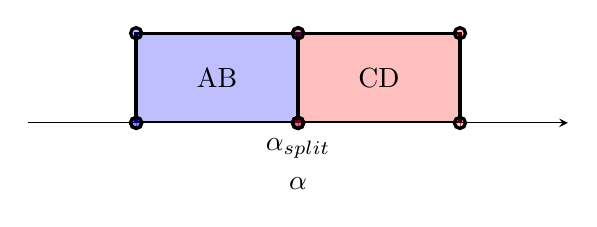
\begin{tikzpicture}
\begin{axis}[
    xmin=0, xmax=1,
    axis x line=bottom,% only show the bottom x axis
    xlabel={$\alpha$},
    xtick={0.2,0.5,0.8},
    xticklabels={$\alo$,$\alpha_{split}$,$\ahi$},
    hide y axis,    
    ymin=0,ymax=5,
    scatter/classes={%
        a={mark=o,draw=black}}
    ]

    \addplot [mark=*,very thick,fill=blue, fill opacity=0.25] coordinates {
        (0.2, 0)
        (0.2, 1)
        (0.5, 1)
        (0.5, 0)
        (0.2, 0)
    };
    \addplot [mark=*,very thick,fill=red, fill opacity=0.25] coordinates {
        (0.5, 0)
        (0.5, 1)
        (0.8, 1)
        (0.8, 0)
        (0.5, 0)
    };
    \node[] at (axis cs: 0.35,0.5) {AB};
    \node[] at (axis cs: 0.65,0.5) {CD};
\end{axis}
\end{tikzpicture}
\end{minipage}
\begin{minipage}{.45\textwidth}
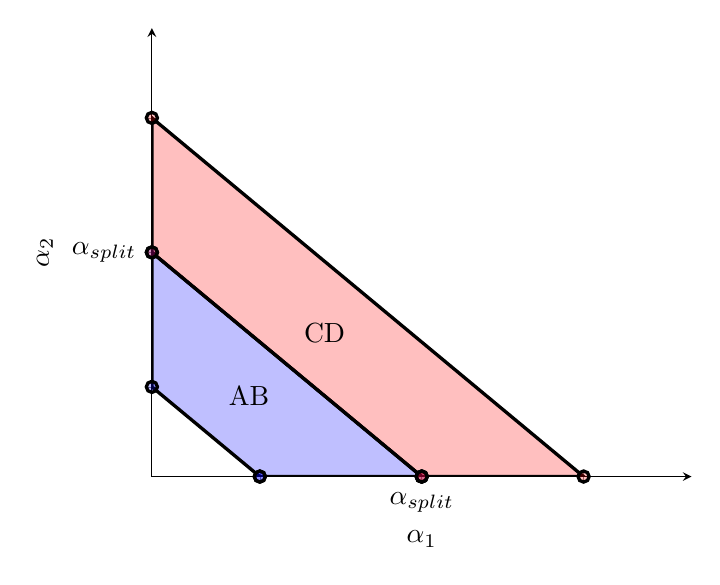
\begin{tikzpicture}
\begin{axis}[
    xmin=0, xmax=1,
    axis x line=bottom,% only show the bottom x axis
    axis y line=left,
    xlabel={$\alpha_1$},
    ylabel={$\alpha_2$},
    xtick={0.2,0.5,0.8},
    xticklabels={$\alo$,$\alpha_{split}$,$\ahi$},  
    ytick={0.2,0.5,0.8},
    yticklabels={$\alo$,$\alpha_{split}$,$\ahi$},  
    ymin=0,ymax=1,
    scatter/classes={%
        a={mark=o,draw=black}}
    ]

    \addplot [mark=*,very thick,fill=blue, fill opacity=0.25] coordinates {
        (0.2, 0)
        (0.5, 0)
        (0, 0.5)
        (0, 0.2)
        (0.2, 0)
    };
    \addplot [mark=*,very thick,fill=red, fill opacity=0.25] coordinates {
        (0.5, 0)
        (0.8, 0)
        (0, 0.8)
        (0, 0.5)
        (0.5, 0)
    };
    \node[] at (axis cs: 0.18,0.18) {AB};
    \node[] at (axis cs: 0.32,0.32) {CD};
\end{axis}
\end{tikzpicture}
\end{minipage}
\caption{While in this work, the split between different merges was based on a linear function $d(\alpha)$ (left), it will be more difficult to evaluate the merges when interpolating with two weight parameters $\alpha_1$ and $\alpha_2$, where the merges will be represented as a convex hull in the $\alpha_1$-$\alpha_2$-space (right).}
\label{fig:convexhull}
\end{figure}

\begin{figure}[h]
\centering
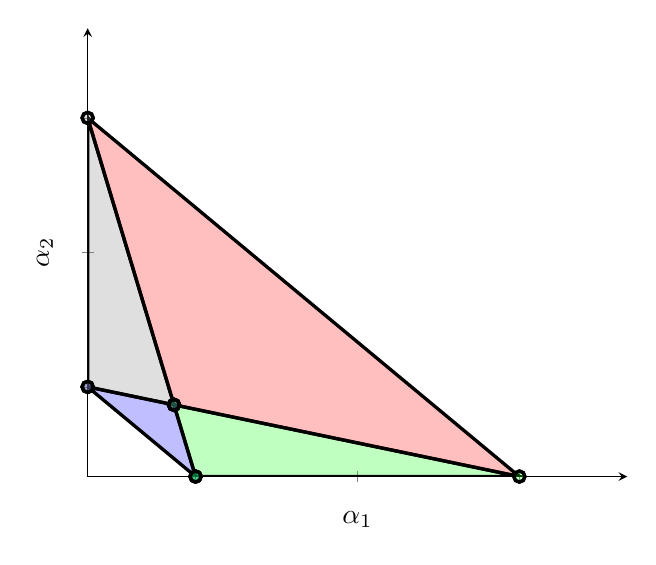
\begin{tikzpicture}
\begin{axis}[
    xmin=0, xmax=1,
    axis x line=bottom,% only show the bottom x axis
    axis y line=left,
    xlabel={$\alpha_1$},
    ylabel={$\alpha_2$},
    xtick={0.2,0.5,0.8},
    xticklabels={$\alo$,,$\ahi$},  
    ytick={0.2,0.5,0.8},
    yticklabels={$\alo$,,$\ahi$},  
    ymin=0,ymax=1,
    scatter/classes={%
        a={mark=o,draw=black}}
    ]
    \addplot [mark=*,very thick,fill=blue, fill opacity=0.25] coordinates {
        (0.2, 0)
        (0, 0.2)
        (0.16, 0.16)
        (0.2, 0)
    };
    \addplot [mark=*,very thick,fill=green, fill opacity=0.25] coordinates {
        (0.2, 0)
        (0.8, 0)
        (0.16, 0.16)
        (0.2, 0)
    };
    \addplot [mark=*,very thick,fill=gray, fill opacity=0.25] coordinates {
        (0, 0.2)
        (0, 0.8)
        (0.16, 0.16)
        (0, 0.2)
    };
    \addplot [mark=o,very thick,fill=red, fill opacity=0.25] coordinates {
        (0.16, 0.16)
        (0.8, 0)
        (0, 0.8)
        (0.16, 0.16)
    };
\end{axis}
\end{tikzpicture}
\caption{Finding the merges in the different regions can be more challenging when interpolating with two weight parameters $\alpha_1$ and $\alpha_2$.}
\label{fig:convexhulls2}
\end{figure}

In addition, we can apply the introduced algorithm to more datasets and data domains, such as the sets contained in the UCI Machine Learning Repository \cite{Dua:2019}. For instance, we could compare different datasets within one specific data domain. Say we evaluate a variety of different image datasets and compare the optimal values of $\alpha$. An interesting observation would be, if we could reuse the optimal parameter from different datasets within the same or even across other domains. In our experiments, we often found similar optimal values in the range $[0.7,0.9]$ while other ranges mostly did not lead to good results (e.g.\ $[0.0, 0.5]$). We could use this knowledge for further experiments by e.g. evaluating only smaller regions or by putting more emphasis on given parameters in general. We can then also evaluate other domains, such as (partially) labeled voice datasets (e.g. the Free Music Archive dataset \cite{fma} or LibriSpeech \cite{librispeech}) and compare the results across different data domains.\\

Also, we can imagine applying this framework to (a) other clustering algorithms than agglomerative hierarchical clustering and (b) other tasks than clustering.

% %\input{Chapters/Chapter4} % Experiment 1

% %\input{Chapters/Chapter5} % Experiment 2

% %\input{Chapters/Chapter6} % Results and Discussion

% %\input{Chapters/Chapter7} % Conclusion

% %% ----------------------------------------------------------------
% % Now begin the Appendices, including them as separate files

% \addtocontents{toc}{\vspace{2em}} % Add a gap in the Contents, for aesthetics

% \appendix % Cue to tell LaTeX that the following 'chapters' are Appendices

% \chapter{The Hungarian Method}
\label{sec:hungarian}

Our goal is to find the best possible matching between two clusterings $C_1^i, ..., C_k^i$ and $C_1^j, ..., C_k^j$. In order to do so, we calculate the cost of matching each possible pair of clusters within the two clusterings. 
% Table \ref{app:hung:distances} shows how such a cost matrix can look like.

% \begin{table}[h]
%     \centering
%     \begin{tabular}{|l | l l l l l|}
%     \hline
%     j\textbackslash i & 1 & 2 & 3 & 4 & 5\\ \hline
%     1 & 20 & 15 & 30 & 50 & 40\\
%     2 & 80 & 10 & 15 & 20 & 30\\
%     3 & 20 & 30 & 50 & 80 & 60\\
%     4 & 30 & 50 & 40 & 20 & 10\\
%     5 & 20 & 30 & 40 & 50 & 25\\ \hline
%     \end{tabular}
%     \caption{In order to determine the optimal matching between two clusterings, we note the pairwise matching costs.}
%     \label{app:hung:distances}
% \end{table}

To find the optimal matching in a brute force way, we have to look at each possible matching. Say we want to match each $i$ to one $j$. For $i = 1$ we can pick from 5 different values of $j$, for $i = 2$ there are 4 potential values of $j$. This will overall result in $k! = 5! = 120$ different combinations, thus the complexity of the brute force approach is $O(k!)$. A more efficient algorithm (especially for higher values of $k$) was introduced by Kuhn and Munkres \cite{kuhn1955hungarian}\cite{munkres1957algorithms}. It consists of three major steps. In the first one, we subtract the row minima from each row. This step is performed in table \ref{app:hung:step1}.

\begin{table}[h]
    \centering
    \begin{tabular}{|l | l l l l l| l |}
    \hline
    j\textbackslash i & 1 & 2 & 3 & 4 & 5 & \\ \hline
    1 & 5 & 0 & 15 & 35 & 25 & (-15)\\
    2 & 70 & 0 & 5 & 10 & 20 & (-10)\\
    3 & 0 & 10 & 30 & 60 & 40 & (-20)\\
    4 & 20 & 40 & 30 & 10 & 0 & (-10)\\
    5 & 0 & 10 & 20 & 30 & 5 & (-20)\\ \hline
    \end{tabular}
    \caption{Hungarian method step 1: Subtract the row minima from each row.}
    \label{app:hung:step1}
\end{table}

After subtracting the row minima, we now also subtract the column minima from each column as shown in table \ref{app:hung:step2}.

\begin{table}[h]
    \centering
    \begin{tabular}{|l | l l l l l |}
    \hline
    j\textbackslash i & 1 & 2 & 3 & 4 & 5\\ \hline
    1 & 5 & 0 & 10 & 25 & 25\\
    2 & 70 & 0 & 0 & 0 & 20\\
    3 & 0 & 10 & 25 & 50 & 40\\
    4 & 20 & 40 & 25 & 0 & 0\\
    5 & 0 & 10 & 15 & 20 & 5\\ \hline
    & - & - & (-5) & (-10) & -\\ \hline
    \end{tabular}
    \caption{Hungarian method step 2: Subtract the column minima from each column.}
    \label{app:hung:step2}
\end{table}

Now we try to find the optimal matching. To do so, we cover all zeros with lines and count the minumum needed lines to do so. Table \ref{app:hung:step3} shows that we need four lines.

\begin{table}[h]
    \centering
    \begin{tabular}{|l | l l l l l |}
    \hline
    j\textbackslash i & 1 & 2 & 3 & 4 & 5\\ \hline
    1 & \cellcolor{orange!25}5 & \cellcolor{orange!50}0 & 10 & 25 & 25\\
    2 & \cellcolor{orange!75}70 & \cellcolor{orange!75}0 & \cellcolor{orange!75}0 & \cellcolor{orange!75}0 & \cellcolor{orange!75}20\\
    3 & \cellcolor{orange!25}0 & \cellcolor{orange!50}10 & 25 & 50 & 40\\
    4 & \cellcolor{orange!75}20 & \cellcolor{orange!75}40 & \cellcolor{orange!75}25 & \cellcolor{orange!75}0 & \cellcolor{orange!75}0\\
    5 & \cellcolor{orange!25}0 & \cellcolor{orange!50}10 & 15 & 20 & 5\\ \hline
    \end{tabular}
    \caption{Hungarian method step 3: Cover all zeros with as few lines as possible.}
    \label{app:hung:step3}
\end{table}

After covering the zeros and counting the lines, we found the optimal matching in case the number of lines equals the number of rows (or columns) in the matrix. As we need four lines and the matrix has five rows in this example, we have to add more zeros. To do that, we subtract the minimum value of the matrix (which is 5 here) from all uncovered values that are not zero and add it to all values that are not zero and covered twice. Now we can again check the needed lines as in table \ref{app:hung:additionalstep}.

\begin{table}[h]
    \centering
    \begin{tabular}{|l | l l l l l |}
    \hline
    j\textbackslash i & 1 & 2 & 3 & 4 & 5\\ \hline
    1 & 5 & 0 & 5 & 20 & 20\\
    2 & 75 & 0 & 0 & 0 & 20\\
    3 & 0 & 10 & 20 & 45 & 35\\
    4 & 25 & 45 & 25 & 0 & 0\\
    5 & 0 & 10 & 10 & 15 & 0\\ \hline
    \end{tabular}
    \begin{tabular}{|l | l l l l l |}
        \hline
        j\textbackslash i & 1 & 2 & 3 & 4 & 5\\ \hline
        1 & \cellcolor{orange!25}5 & \cellcolor{orange!50}0 & 5 & 20 & 20\\
        2 & \cellcolor{orange!75}75 & \cellcolor{orange!75}0 & \cellcolor{orange!75}0 & \cellcolor{orange!75}0 & \cellcolor{orange!75}20\\
        3 & \cellcolor{orange!25}0 & \cellcolor{orange!50}10 & 20 & 45 & 35\\
        4 & \cellcolor{orange!75}25 & \cellcolor{orange!75}45 & \cellcolor{orange!75}25 & \cellcolor{orange!75}0 & \cellcolor{orange!75}0\\
        5 & \cellcolor{orange!100}0 & \cellcolor{orange!100}10 & \cellcolor{orange!100}10 & \cellcolor{orange!100}15 & \cellcolor{orange!100}0\\ \hline
    \end{tabular}
    \caption{Hungarian method additional step: Create more zeroes until the number of minimal needed lines to cover all zeros matches the number of rows.}
    \label{app:hung:additionalstep}
\end{table}

This will then result in the assignment seen in table \ref{app:hung:assignment}. Applying the matching to the input matrix then gives the optimal cost by summing the optimal values. For this example the optimal cost is then 95.

\begin{table}[h]
    \centering
    \begin{tabular}{|l | l l l l l |}
    \hline
    j\textbackslash i & 1 & 2 & 3 & 4 & 5\\ \hline
    1 & 5 & \cellcolor{blue!25}0 & 5 & 20 & 20\\
    2 & 75 & 0 & \cellcolor{blue!25}0 & 0 & 20\\
    3 & \cellcolor{blue!25}0 & 10 & 20 & 45 & 35\\
    4 & 25 & 45 & 25 & \cellcolor{blue!25}0 & 0\\
    5 & 0 & 10 & 10 & 15 & \cellcolor{blue!25}0\\ \hline
    \end{tabular}
    \begin{tabular}{|l | l l l l l|}
        \hline
        j\textbackslash i & 1 & 2 & 3 & 4 & 5\\ \hline
        1 & 20 & \cellcolor{blue!25}15 & 30 & 50 & 40\\
        2 & 80 & 10 & \cellcolor{blue!25}15 & 20 & 30\\
        3 & \cellcolor{blue!25}20 & 30 & 50 & 80 & 60\\
        4 & 30 & 50 & 40 & \cellcolor{blue!25}20 & 10\\
        5 & 20 & 30 & 40 & 50 & \cellcolor{blue!25}25\\ \hline
    \end{tabular}
    \caption{Result of the Hungarian method: The optimal matching between two clusterings.}
    \label{app:hung:assignment}
\end{table}	% Appendix Title

% \chapter{Convolutional Neural Network Architecture for Feature Extraction}
\label{sec:cnnarchitecture}

\begin{figure}[H]
    \centering
    \includegraphics[width=0.6\textwidth]{images/model}
    \caption{We use a small Convolutional Neural Network (CNN) architecture to create meaningful features for the MNIST and the Omniglot data.}
    \label{fig:model}
\end{figure} % Appendix Title

% %\chapter{Additional NELL Results}
\label{app:nell}

Here we show the results of all the 30 different used entities. We used a maximum of 1,000 points for each entity, however for some of them less samples were given. We show both interpolating between average and complete and between single and complete linkage in the following figures.

\begin{figure}[h]
\centering
\begin{minipage}{.24\textwidth}
  \centering
  \subcaptionbox{Animal}
  {\includegraphics[width=\linewidth]{plots/nell-ac/animal}}
\end{minipage}
\begin{minipage}{.24\textwidth}
  \centering
  \subcaptionbox{Arthropod}
  {\includegraphics[width=\linewidth]{plots/nell-ac/arthropod}}
\end{minipage}
\begin{minipage}{.24\textwidth}
  \centering
  \subcaptionbox{Attraction}
  {\includegraphics[width=\linewidth]{plots/nell-ac/attraction}}
\end{minipage}
\begin{minipage}{.24\textwidth}
  \centering
  \subcaptionbox{Beverage}
  {\includegraphics[width=\linewidth]{plots/nell-ac/beverage}}
\end{minipage}
\begin{minipage}{.24\textwidth}
  \centering
  \subcaptionbox{Bodypart}
  {\includegraphics[width=\linewidth]{plots/nell-ac/bodypart}}
\end{minipage}
\begin{minipage}{.24\textwidth}
  \centering
  \subcaptionbox{Building}
  {\includegraphics[width=\linewidth]{plots/nell-ac/building}}
\end{minipage}
\begin{minipage}{.24\textwidth}
  \centering
  \subcaptionbox{Company}
  {\includegraphics[width=\linewidth]{plots/nell-ac/company}}
\end{minipage}
\begin{minipage}{.24\textwidth}
  \centering
  \subcaptionbox{Creative Work}
  {\includegraphics[width=\linewidth]{plots/nell-ac/creativework}}
\end{minipage}
\begin{minipage}{.24\textwidth}
  \centering
  \subcaptionbox{Date}
  {\includegraphics[width=\linewidth]{plots/nell-ac/date}}
\end{minipage}
\begin{minipage}{.24\textwidth}
  \centering
  \subcaptionbox{Event}
  {\includegraphics[width=\linewidth]{plots/nell-ac/event}}
\end{minipage}
\begin{minipage}{.24\textwidth}
  \centering
  \subcaptionbox{Food}
  {\includegraphics[width=\linewidth]{plots/nell-ac/food}}
\end{minipage}
\begin{minipage}{.24\textwidth}
  \centering
  \subcaptionbox{Fruit}
  {\includegraphics[width=\linewidth]{plots/nell-ac/fruit}}
\end{minipage}
\begin{minipage}{.24\textwidth}
  \centering
  \subcaptionbox{Game}
  {\includegraphics[width=\linewidth]{plots/nell-ac/game}}
\end{minipage}
\begin{minipage}{.24\textwidth}
  \centering
  \subcaptionbox{Household Item}
  {\includegraphics[width=\linewidth]{plots/nell-ac/householditem}}
\end{minipage}
\begin{minipage}{.24\textwidth}
  \centering
  \subcaptionbox{Invertebrate}
  {\includegraphics[width=\linewidth]{plots/nell-ac/invertebrate}}
\end{minipage}
\begin{minipage}{.24\textwidth}
  \centering
  \subcaptionbox{Location}
  {\includegraphics[width=\linewidth]{plots/nell-ac/location}}
\end{minipage}
\end{figure}
\begin{figure}[h]\ContinuedFloat
\centering
\begin{minipage}{.24\textwidth}
  \centering
  \subcaptionbox{Mediacompany}
  {\includegraphics[width=\linewidth]{plots/nell-ac/mediacompany}}
\end{minipage}
\begin{minipage}{.24\textwidth}
  \centering
  \subcaptionbox{Organization}
  {\includegraphics[width=\linewidth]{plots/nell-ac/organization}}
\end{minipage}
\begin{minipage}{.24\textwidth}
  \centering
  \subcaptionbox{Person}
  {\includegraphics[width=\linewidth]{plots/nell-ac/person}}
\end{minipage}
\begin{minipage}{.24\textwidth}
  \centering
  \subcaptionbox{Person by Location}
  {\includegraphics[width=\linewidth]{plots/nell-ac/personbylocation}}
\end{minipage}
\begin{minipage}{.24\textwidth}
  \centering
  \subcaptionbox{Person NA}
  {\includegraphics[width=\linewidth]{plots/nell-ac/personnorthamerica}}
\end{minipage}
\begin{minipage}{.24\textwidth}
  \centering
  \subcaptionbox{Physiological Condition}
  {\includegraphics[width=\linewidth]{plots/nell-ac/physiologicalcondition}}
\end{minipage}
\begin{minipage}{.24\textwidth}
  \centering
  \subcaptionbox{Politics Group}
  {\includegraphics[width=\linewidth]{plots/nell-ac/politicsgroup}}
\end{minipage}
\begin{minipage}{.24\textwidth}
  \centering
  \subcaptionbox{Product}
  {\includegraphics[width=\linewidth]{plots/nell-ac/Product}}
\end{minipage}
\begin{minipage}{.24\textwidth}
  \centering
  \subcaptionbox{Publication}
  {\includegraphics[width=\linewidth]{plots/nell-ac/publication}}
\end{minipage}
\begin{minipage}{.24\textwidth}
  \centering
  \subcaptionbox{School}
  {\includegraphics[width=\linewidth]{plots/nell-ac/school}}
\end{minipage}
\begin{minipage}{.24\textwidth}
  \centering
  \subcaptionbox{Software}
  {\includegraphics[width=\linewidth]{plots/nell-ac/software}}
\end{minipage}
\begin{minipage}{.24\textwidth}
  \centering
  \subcaptionbox{Sports Event}
  {\includegraphics[width=\linewidth]{plots/nell-ac/sportsevent}}
\end{minipage}
\begin{minipage}{.24\textwidth}
  \centering
  \subcaptionbox{Traditional Game}
  {\includegraphics[width=\linewidth]{plots/nell-ac/traditionalgame}}
\end{minipage}
\begin{minipage}{.24\textwidth}
  \centering
  \subcaptionbox{Vertebrate}
  {\includegraphics[width=\linewidth]{plots/nell-ac/vertebrate}}
\end{minipage}
\begin{minipage}{.24\textwidth}
  \centering
  \subcaptionbox{Visualizable Attribute}
  {\includegraphics[width=\linewidth]{plots/nell-ac/visualizableattribute}}
\end{minipage}
\begin{minipage}{.24\textwidth}
  \centering
  \subcaptionbox{Website}
  {\includegraphics[width=\linewidth]{plots/nell-ac/website}}
\end{minipage}
\caption{Interpolating between average and complete linkage for the NELL data.}
\end{figure}

\begin{figure}[h]
\centering
\begin{minipage}{.24\textwidth}
  \centering
  \subcaptionbox{Animal}
  {\includegraphics[width=\linewidth]{plots/nell-sc/animal}}
\end{minipage}
\begin{minipage}{.24\textwidth}
  \centering
  \subcaptionbox{Arthropod}
  {\includegraphics[width=\linewidth]{plots/nell-sc/arthropod}}
\end{minipage}
\begin{minipage}{.24\textwidth}
  \centering
  \subcaptionbox{Attraction}
  {\includegraphics[width=\linewidth]{plots/nell-sc/attraction}}
\end{minipage}
\begin{minipage}{.24\textwidth}
  \centering
  \subcaptionbox{Beverage}
  {\includegraphics[width=\linewidth]{plots/nell-sc/beverage}}
\end{minipage}
\begin{minipage}{.24\textwidth}
  \centering
  \subcaptionbox{Bodypart}
  {\includegraphics[width=\linewidth]{plots/nell-sc/bodypart}}
\end{minipage}
\begin{minipage}{.24\textwidth}
  \centering
  \subcaptionbox{Building}
  {\includegraphics[width=\linewidth]{plots/nell-sc/building}}
\end{minipage}
\begin{minipage}{.24\textwidth}
  \centering
  \subcaptionbox{Company}
  {\includegraphics[width=\linewidth]{plots/nell-sc/company}}
\end{minipage}
\begin{minipage}{.24\textwidth}
  \centering
  \subcaptionbox{Creative Work}
  {\includegraphics[width=\linewidth]{plots/nell-sc/creativework}}
\end{minipage}
\begin{minipage}{.24\textwidth}
  \centering
  \subcaptionbox{Date}
  {\includegraphics[width=\linewidth]{plots/nell-sc/date}}
\end{minipage}
\begin{minipage}{.24\textwidth}
  \centering
  \subcaptionbox{Event}
  {\includegraphics[width=\linewidth]{plots/nell-sc/event}}
\end{minipage}
\begin{minipage}{.24\textwidth}
  \centering
  \subcaptionbox{Food}
  {\includegraphics[width=\linewidth]{plots/nell-sc/food}}
\end{minipage}
\begin{minipage}{.24\textwidth}
  \centering
  \subcaptionbox{Fruit}
  {\includegraphics[width=\linewidth]{plots/nell-sc/fruit}}
\end{minipage}
\begin{minipage}{.24\textwidth}
  \centering
  \subcaptionbox{Game}
  {\includegraphics[width=\linewidth]{plots/nell-sc/game}}
\end{minipage}
\begin{minipage}{.24\textwidth}
  \centering
  \subcaptionbox{Household Item}
  {\includegraphics[width=\linewidth]{plots/nell-sc/householditem}}
\end{minipage}
\begin{minipage}{.24\textwidth}
  \centering
  \subcaptionbox{Invertebrate}
  {\includegraphics[width=\linewidth]{plots/nell-sc/invertebrate}}
\end{minipage}
\begin{minipage}{.24\textwidth}
  \centering
  \subcaptionbox{Location}
  {\includegraphics[width=\linewidth]{plots/nell-sc/location}}
\end{minipage}
\begin{minipage}{.24\textwidth}
  \centering
  \subcaptionbox{Mediacompany}
  {\includegraphics[width=\linewidth]{plots/nell-sc/mediacompany}}
\end{minipage}
\begin{minipage}{.24\textwidth}
  \centering
  \subcaptionbox{Organization}
  {\includegraphics[width=\linewidth]{plots/nell-sc/organization}}
\end{minipage}
\begin{minipage}{.24\textwidth}
  \centering
  \subcaptionbox{Person}
  {\includegraphics[width=\linewidth]{plots/nell-sc/person}}
\end{minipage}
\begin{minipage}{.24\textwidth}
  \centering
  \subcaptionbox{Person by Location}
  {\includegraphics[width=\linewidth]{plots/nell-sc/personbylocation}}
\end{minipage}
\end{figure}
\begin{figure}[h]\ContinuedFloat
\centering
\begin{minipage}{.24\textwidth}
  \centering
  \subcaptionbox{Person NA}
  {\includegraphics[width=\linewidth]{plots/nell-sc/personnorthamerica}}
\end{minipage}
\begin{minipage}{.24\textwidth}
  \centering
  \subcaptionbox{Physiological Condition}
  {\includegraphics[width=\linewidth]{plots/nell-sc/physiologicalcondition}}
\end{minipage}
\begin{minipage}{.24\textwidth}
  \centering
  \subcaptionbox{Politics Group}
  {\includegraphics[width=\linewidth]{plots/nell-sc/politicsgroup}}
\end{minipage}
\begin{minipage}{.24\textwidth}
  \centering
  \subcaptionbox{Product}
  {\includegraphics[width=\linewidth]{plots/nell-sc/Product}}
\end{minipage}
\begin{minipage}{.24\textwidth}
  \centering
  \subcaptionbox{Publication}
  {\includegraphics[width=\linewidth]{plots/nell-sc/publication}}
\end{minipage}
\begin{minipage}{.24\textwidth}
  \centering
  \subcaptionbox{School}
  {\includegraphics[width=\linewidth]{plots/nell-sc/school}}
\end{minipage}
\begin{minipage}{.24\textwidth}
  \centering
  \subcaptionbox{Software}
  {\includegraphics[width=\linewidth]{plots/nell-sc/software}}
\end{minipage}
\begin{minipage}{.24\textwidth}
  \centering
  \subcaptionbox{Sports Event}
  {\includegraphics[width=\linewidth]{plots/nell-sc/sportsevent}}
\end{minipage}
\begin{minipage}{.24\textwidth}
  \centering
  \subcaptionbox{Traditional Game}
  {\includegraphics[width=\linewidth]{plots/nell-sc/traditionalgame}}
\end{minipage}
\begin{minipage}{.24\textwidth}
  \centering
  \subcaptionbox{Vertebrate}
  {\includegraphics[width=\linewidth]{plots/nell-sc/vertebrate}}
\end{minipage}
\begin{minipage}{.24\textwidth}
  \centering
  \subcaptionbox{Visualizable Attribute}
  {\includegraphics[width=\linewidth]{plots/nell-sc/visualizableattribute}}
\end{minipage}
\begin{minipage}{.24\textwidth}
  \centering
  \subcaptionbox{Website}
  {\includegraphics[width=\linewidth]{plots/nell-sc/website}}
\end{minipage}
\caption{Interpolating between single and complete linkage for the NELL data.}
\end{figure} % Appendix Title

% \addtocontents{toc}{\vspace{2em}}  % Add a gap in the Contents, for aesthetics
% \backmatter

% %% ----------------------------------------------------------------
% \label{Bibliography}
% \lhead{\emph{Bibliography}}  % Change the left side page header to "Bibliography"
% \bibliographystyle{unsrtnat}  % Use the "unsrtnat" BibTeX style for formatting the Bibliography
% \bibliography{Bibliography}  % The references (bibliography) information are stored in the file named "Bibliography.bib"

% \end{document}  % The End
% %% ----------------------------------------------------------------